\documentclass[twoside]{book}

% Packages required by doxygen
\usepackage{fixltx2e}
\usepackage{calc}
\usepackage{doxygen}
\usepackage[export]{adjustbox} % also loads graphicx
\usepackage{graphicx}
\usepackage[utf8]{inputenc}
\usepackage{makeidx}
\usepackage{multicol}
\usepackage{multirow}
\PassOptionsToPackage{warn}{textcomp}
\usepackage{textcomp}
\usepackage[nointegrals]{wasysym}
\usepackage[table]{xcolor}

% Font selection
\usepackage[T1]{fontenc}
\usepackage[scaled=.90]{helvet}
\usepackage{courier}
\usepackage{amssymb}
\usepackage{sectsty}
\renewcommand{\familydefault}{\sfdefault}
\allsectionsfont{%
  \fontseries{bc}\selectfont%
  \color{darkgray}%
}
\renewcommand{\DoxyLabelFont}{%
  \fontseries{bc}\selectfont%
  \color{darkgray}%
}
\newcommand{\+}{\discretionary{\mbox{\scriptsize$\hookleftarrow$}}{}{}}

% Page & text layout
\usepackage{geometry}
\geometry{%
  a4paper,%
  top=2.5cm,%
  bottom=2.5cm,%
  left=2.5cm,%
  right=2.5cm%
}
\tolerance=750
\hfuzz=15pt
\hbadness=750
\setlength{\emergencystretch}{15pt}
\setlength{\parindent}{0cm}
\setlength{\parskip}{3ex plus 2ex minus 2ex}
\makeatletter
\renewcommand{\paragraph}{%
  \@startsection{paragraph}{4}{0ex}{-1.0ex}{1.0ex}{%
    \normalfont\normalsize\bfseries\SS@parafont%
  }%
}
\renewcommand{\subparagraph}{%
  \@startsection{subparagraph}{5}{0ex}{-1.0ex}{1.0ex}{%
    \normalfont\normalsize\bfseries\SS@subparafont%
  }%
}
\makeatother

% Headers & footers
\usepackage{fancyhdr}
\pagestyle{fancyplain}
\fancyhead[LE]{\fancyplain{}{\bfseries\thepage}}
\fancyhead[CE]{\fancyplain{}{}}
\fancyhead[RE]{\fancyplain{}{\bfseries\leftmark}}
\fancyhead[LO]{\fancyplain{}{\bfseries\rightmark}}
\fancyhead[CO]{\fancyplain{}{}}
\fancyhead[RO]{\fancyplain{}{\bfseries\thepage}}
\fancyfoot[LE]{\fancyplain{}{}}
\fancyfoot[CE]{\fancyplain{}{}}
\fancyfoot[RE]{\fancyplain{}{\bfseries\scriptsize Generated by Doxygen }}
\fancyfoot[LO]{\fancyplain{}{\bfseries\scriptsize Generated by Doxygen }}
\fancyfoot[CO]{\fancyplain{}{}}
\fancyfoot[RO]{\fancyplain{}{}}
\renewcommand{\footrulewidth}{0.4pt}
\renewcommand{\chaptermark}[1]{%
  \markboth{#1}{}%
}
\renewcommand{\sectionmark}[1]{%
  \markright{\thesection\ #1}%
}

% Indices & bibliography
\usepackage{natbib}
\usepackage[titles]{tocloft}
\setcounter{tocdepth}{3}
\setcounter{secnumdepth}{5}
\makeindex

% Hyperlinks (required, but should be loaded last)
\usepackage{ifpdf}
\ifpdf
  \usepackage[pdftex,pagebackref=true]{hyperref}
\else
  \usepackage[ps2pdf,pagebackref=true]{hyperref}
\fi
\hypersetup{%
  colorlinks=true,%
  linkcolor=blue,%
  citecolor=blue,%
  unicode%
}

% Custom commands
\newcommand{\clearemptydoublepage}{%
  \newpage{\pagestyle{empty}\cleardoublepage}%
}

\usepackage{caption}
\captionsetup{labelsep=space,justification=centering,font={bf},singlelinecheck=off,skip=4pt,position=top}

%===== C O N T E N T S =====

\begin{document}

% Titlepage & ToC
\hypersetup{pageanchor=false,
             bookmarksnumbered=true,
             pdfencoding=unicode
            }
\pagenumbering{roman}
\begin{titlepage}
\vspace*{7cm}
\begin{center}%
{\Large V\+R\+E\+P-\/\+Plugin for paparazzi communication to control simulated copters }\\
\vspace*{1cm}
{\large Generated by Doxygen 1.8.11}\\
\end{center}
\end{titlepage}
\clearemptydoublepage
\tableofcontents
\clearemptydoublepage
\pagenumbering{arabic}
\hypersetup{pageanchor=true}

%--- Begin generated contents ---
\chapter{V\+R\+EP Integrated paparazzi simulation (V\+I\+P\+S\+IM?)}
\label{index}\hypertarget{index}{}\hypertarget{index_intro_sec}{}\section{Introduction}\label{index_intro_sec}
This V-\/\+R\+EP plugin provides a framework for integrating the native Paparazzi control-\/loop for U\+A\+Vs into the 3D virtual-\/ robot experimentation platform V-\/\+R\+EP, created for the simulation of the quadcopters in the Otto-\/\+Von-\/\+Guericke University Swarm\+Lab.~\newline
 It works by feeding the Paparazzi flight dynamics model data obtained from the 3D simulation environment provided by V-\/\+R\+EP, and then exectuing the commands Paparazzi provides based on that data.\hypertarget{index_install_sec}{}\section{Installation and usage}\label{index_install_sec}
\hypertarget{index_step1}{}\subsection{Step 1\+: Repositories and V-\/\+R\+EP}\label{index_step1}
Install V-\/\+R\+EP and Paparazzi. ~\newline
 Clone \href{https://github.com/ovgu-FINken/Simulation/tree/paparazziSimSingle}{\tt https\+://github.\+com/ovgu-\/\+F\+I\+Nken/\+Simulation/tree/paparazzi\+Sim\+Single} for the V-\/\+R\+EP code(branch paparazzi\+Sim\+Single) ~\newline
 and \href{https://github.com/ovgu-FINken/paparazzi}{\tt https\+://github.\+com/ovgu-\/\+F\+I\+Nken/paparazzi} (branch vrep\+Sim\+Orig).\hypertarget{index_step2}{}\subsection{Step 2\+: Dependencies and libraries}\label{index_step2}
Install boost and eigen3. Make sure to add the variables P\+A\+P\+A\+R\+A\+Z\+Z\+I\+\_\+\+H\+O\+ME and V\+R\+E\+P\+\_\+\+H\+O\+ME to you environment variables, pointing to the respective root folders.\hypertarget{index_step3}{}\subsection{Step 3\+: Running the simulation}\label{index_step3}
To run the simulation, open vrep and load the scene finken\+Rotated.\+ccc provided in the simulation repository. If you wish to build your own scene, make sure to include the \char`\"{}scriptloader\char`\"{} object in as in the example scene or the plugin will not work.~\newline
 In paparazzi, select the aircraft \char`\"{}test\char`\"{} and build the target nps.

Then press play on the vrep simulation, followed by executing the paparazzi simulation. 
\chapter{Todo List}
\label{todo}
\hypertarget{todo}{}

\begin{DoxyRefList}
\item[\label{todo__todo000005}%
\hypertarget{todo__todo000005}{}%
Class \hyperlink{classAsync__Server}{Async\+\_\+\+Server} ]move to separate.\+cpp file  
\item[\label{todo__todo000001}%
\hypertarget{todo__todo000001}{}%
Class \hyperlink{classAttitudeSensor}{Attitude\+Sensor} ]actually use this for attitude calculation. 

actually use this for attitude calculation.  
\item[\label{todo__todo000003}%
\hypertarget{todo__todo000003}{}%
Class \hyperlink{classLogLine}{Log\+Line} ]cleanup code from superfluous debug logging  
\item[\label{todo__todo000006}%
\hypertarget{todo__todo000006}{}%
Class \hyperlink{classPositionSensor}{Position\+Sensor} ]actually use this in the sim  
\item[\label{todo__todo000007}%
\hypertarget{todo__todo000007}{}%
Class \hyperlink{classSonar}{Sonar} ]actually use this in the sim  
\item[\label{todo__todo000004}%
\hypertarget{todo__todo000004}{}%
Class \hyperlink{classVrepLog}{Vrep\+Log} ]cleanup code from superfluous debug logging 
\end{DoxyRefList}
\chapter{Namespace Index}
\section{Namespace List}
Here is a list of all namespaces with brief descriptions\+:\begin{DoxyCompactList}
\item\contentsline{section}{\hyperlink{namespaceboost}{boost} }{\pageref{namespaceboost}}{}
\item\contentsline{section}{\hyperlink{namespaceboost_1_1serialization}{boost\+::serialization} }{\pageref{namespaceboost_1_1serialization}}{}
\end{DoxyCompactList}

\chapter{Hierarchical Index}
\section{Class Hierarchy}
This inheritance list is sorted roughly, but not completely, alphabetically\+:\begin{DoxyCompactList}
\item \contentsline{section}{Async\+\_\+\+Server}{\pageref{classAsync__Server}}{}
\item \contentsline{section}{Finken}{\pageref{classFinken}}{}
\item \contentsline{section}{Log}{\pageref{classLog}}{}
\item \contentsline{section}{Log\+Line}{\pageref{classLogLine}}{}
\item \contentsline{section}{Rotor}{\pageref{classRotor}}{}
\item \contentsline{section}{Sensor}{\pageref{classSensor}}{}
\begin{DoxyCompactList}
\item \contentsline{section}{Attitude\+Sensor}{\pageref{classAttitudeSensor}}{}
\item \contentsline{section}{Height\+Sensor}{\pageref{classHeightSensor}}{}
\item \contentsline{section}{Position\+Sensor}{\pageref{classPositionSensor}}{}
\item \contentsline{section}{Sonar}{\pageref{classSonar}}{}
\end{DoxyCompactList}
\item \contentsline{section}{Vrep\+Log}{\pageref{classVrepLog}}{}
\item \contentsline{section}{V\+R\+E\+P\+Plugin}{\pageref{classVREPPlugin}}{}
\begin{DoxyCompactList}
\item \contentsline{section}{Finken\+Plugin}{\pageref{classFinkenPlugin}}{}
\end{DoxyCompactList}
\end{DoxyCompactList}

\chapter{Class Index}
\section{Class List}
Here are the classes, structs, unions and interfaces with brief descriptions\+:\begin{DoxyCompactList}
\item\contentsline{section}{\hyperlink{classAsync__Server}{Async\+\_\+\+Server} \\*Asynchronous (boost\+::\+Asio) Server class to accept new paparazzi connections and pair them with a vrep copter }{\pageref{classAsync__Server}}{}
\item\contentsline{section}{\hyperlink{classAttitudeSensor}{Attitude\+Sensor} \\*Currently unused class for an attitude sensor }{\pageref{classAttitudeSensor}}{}
\item\contentsline{section}{\hyperlink{classFinken}{Finken} \\*\hyperlink{classFinken}{Finken} class for handling any data exchanges between a F\+I\+Nken and Paparazzi }{\pageref{classFinken}}{}
\item\contentsline{section}{\hyperlink{classFinkenPlugin}{Finken\+Plugin} \\*The actual finken plugin }{\pageref{classFinkenPlugin}}{}
\item\contentsline{section}{\hyperlink{classHeightSensor}{Height\+Sensor} \\*Class implementing a heightsensor }{\pageref{classHeightSensor}}{}
\item\contentsline{section}{\hyperlink{classLog}{Log} \\*Baisc logging class }{\pageref{classLog}}{}
\item\contentsline{section}{\hyperlink{classLogLine}{Log\+Line} \\*Class for annotating log with time points }{\pageref{classLogLine}}{}
\item\contentsline{section}{\hyperlink{classPositionSensor}{Position\+Sensor} \\*Wrapper to disguise vrep A\+PI calls as a position sensor }{\pageref{classPositionSensor}}{}
\item\contentsline{section}{\hyperlink{classRotor}{Rotor} \\*Implementation of a force sensor as a rotor }{\pageref{classRotor}}{}
\item\contentsline{section}{\hyperlink{classSensor}{Sensor} \\*Base \hyperlink{classSensor}{Sensor} class, all sensors should inherit from this }{\pageref{classSensor}}{}
\item\contentsline{section}{\hyperlink{classSonar}{Sonar} \\*Implementation of a proximitysensor as sonar }{\pageref{classSonar}}{}
\item\contentsline{section}{\hyperlink{classVrepLog}{Vrep\+Log} \\*Class for creating a log file }{\pageref{classVrepLog}}{}
\item\contentsline{section}{\hyperlink{classVREPPlugin}{V\+R\+E\+P\+Plugin} \\*Base vrepplugin class }{\pageref{classVREPPlugin}}{}
\end{DoxyCompactList}

\chapter{File Index}
\section{File List}
Here is a list of all documented files with brief descriptions\+:\begin{DoxyCompactList}
\item\contentsline{section}{\hyperlink{attitudesensor_8cpp}{attitudesensor.\+cpp} }{\pageref{attitudesensor_8cpp}}{}
\item\contentsline{section}{\hyperlink{attitudesensor_8h}{attitudesensor.\+h} }{\pageref{attitudesensor_8h}}{}
\item\contentsline{section}{\hyperlink{finken_8cpp}{finken.\+cpp} }{\pageref{finken_8cpp}}{}
\item\contentsline{section}{\hyperlink{finken_8h}{finken.\+h} \\*Header for the finken implementation }{\pageref{finken_8h}}{}
\item\contentsline{section}{\hyperlink{finkenplugin_8cpp}{finkenplugin.\+cpp} }{\pageref{finkenplugin_8cpp}}{}
\item\contentsline{section}{\hyperlink{heightsensor_8cpp}{heightsensor.\+cpp} }{\pageref{heightsensor_8cpp}}{}
\item\contentsline{section}{{\bfseries heightsensor.\+h} }{\pageref{heightsensor_8h}}{}
\item\contentsline{section}{{\bfseries log.\+h} }{\pageref{log_8h}}{}
\item\contentsline{section}{\hyperlink{positionsensor_8cpp}{positionsensor.\+cpp} }{\pageref{positionsensor_8cpp}}{}
\item\contentsline{section}{{\bfseries positionsensor.\+h} }{\pageref{positionsensor_8h}}{}
\item\contentsline{section}{\hyperlink{rotor_8cpp}{rotor.\+cpp} }{\pageref{rotor_8cpp}}{}
\item\contentsline{section}{{\bfseries rotor.\+h} }{\pageref{rotor_8h}}{}
\item\contentsline{section}{\hyperlink{sensor_8cpp}{sensor.\+cpp} }{\pageref{sensor_8cpp}}{}
\item\contentsline{section}{{\bfseries sensor.\+h} }{\pageref{sensor_8h}}{}
\item\contentsline{section}{\hyperlink{skeleton_8cpp}{skeleton.\+cpp} \\*Basic functionality for communication with the running vrep Simulation" }{\pageref{skeleton_8cpp}}{}
\item\contentsline{section}{\hyperlink{sonar_8cpp}{sonar.\+cpp} }{\pageref{sonar_8cpp}}{}
\item\contentsline{section}{{\bfseries sonar.\+h} }{\pageref{sonar_8h}}{}
\item\contentsline{section}{\hyperlink{threadSync_8cpp}{thread\+Sync.\+cpp} \\*Currently unused structures for syncing several F\+I\+Nken threads }{\pageref{threadSync_8cpp}}{}
\item\contentsline{section}{{\bfseries vrepplugin.\+h} }{\pageref{vrepplugin_8h}}{}
\end{DoxyCompactList}

\chapter{Namespace Documentation}
\hypertarget{namespaceboost}{}\section{boost Namespace Reference}
\label{namespaceboost}\index{boost@{boost}}
\subsection*{Namespaces}
\begin{DoxyCompactItemize}
\item 
 \hyperlink{namespaceboost_1_1serialization}{serialization}
\end{DoxyCompactItemize}

\hypertarget{namespaceboost_1_1serialization}{}\section{boost\+:\+:serialization Namespace Reference}
\label{namespaceboost_1_1serialization}\index{boost\+::serialization@{boost\+::serialization}}
\subsection*{Functions}
\begin{DoxyCompactItemize}
\item 
{\footnotesize template$<$typename T , int rows, int cols, class Archive $>$ }\\void \hyperlink{namespaceboost_1_1serialization_aa7021b16faca824017a33df205f44c01}{save} (Archive \&ar, const \+::\hyperlink{test_8cpp_a645222978e81acfb2523a9bce34aecc0}{Eigen\+::\+Matrix}$<$ T, rows, cols $>$ \&m, unsigned int v)
\item 
{\footnotesize template$<$typename T , int R, int C, class Archive $>$ }\\void \hyperlink{namespaceboost_1_1serialization_a76faf89a36520a5181fe7464aec003fe}{load} (Archive \&ar,\+::\hyperlink{test_8cpp_a645222978e81acfb2523a9bce34aecc0}{Eigen\+::\+Matrix}$<$ T, R, C $>$ \&m, unsigned int v)
\item 
{\footnotesize template$<$typename T , int rows, int cols, class Archive $>$ }\\void \hyperlink{namespaceboost_1_1serialization_a5839810cadeccc13a50f63a8cae475a5}{serialize} (Archive \&ar,\+::\hyperlink{test_8cpp_a645222978e81acfb2523a9bce34aecc0}{Eigen\+::\+Matrix}$<$ T, rows, cols $>$ \&m, unsigned int file\+\_\+version)
\end{DoxyCompactItemize}


\subsection{Function Documentation}
\index{boost\+::serialization@{boost\+::serialization}!load@{load}}
\index{load@{load}!boost\+::serialization@{boost\+::serialization}}
\subsubsection[{\texorpdfstring{load(\+Archive \&ar,\+::\+Eigen\+::\+Matrix$<$ T, R, C $>$ \&m, unsigned int v)}{load(Archive &ar,::Eigen::Matrix< T, R, C > &m, unsigned int v)}}]{\setlength{\rightskip}{0pt plus 5cm}template$<$typename T , int R, int C, class Archive $>$ void boost\+::serialization\+::load (
\begin{DoxyParamCaption}
\item[{Archive \&}]{ar, }
\item[{\+::{\bf Eigen\+::\+Matrix}$<$ T, R, C $>$ \&}]{m, }
\item[{unsigned int}]{v}
\end{DoxyParamCaption}
)\hspace{0.3cm}{\ttfamily [inline]}}\hypertarget{namespaceboost_1_1serialization_a76faf89a36520a5181fe7464aec003fe}{}\label{namespaceboost_1_1serialization_a76faf89a36520a5181fe7464aec003fe}
\index{boost\+::serialization@{boost\+::serialization}!save@{save}}
\index{save@{save}!boost\+::serialization@{boost\+::serialization}}
\subsubsection[{\texorpdfstring{save(\+Archive \&ar, const \+::\+Eigen\+::\+Matrix$<$ T, rows, cols $>$ \&m, unsigned int v)}{save(Archive &ar, const ::Eigen::Matrix< T, rows, cols > &m, unsigned int v)}}]{\setlength{\rightskip}{0pt plus 5cm}template$<$typename T , int rows, int cols, class Archive $>$ void boost\+::serialization\+::save (
\begin{DoxyParamCaption}
\item[{Archive \&}]{ar, }
\item[{const \+::{\bf Eigen\+::\+Matrix}$<$ T, rows, cols $>$ \&}]{m, }
\item[{unsigned int}]{v}
\end{DoxyParamCaption}
)\hspace{0.3cm}{\ttfamily [inline]}}\hypertarget{namespaceboost_1_1serialization_aa7021b16faca824017a33df205f44c01}{}\label{namespaceboost_1_1serialization_aa7021b16faca824017a33df205f44c01}
\index{boost\+::serialization@{boost\+::serialization}!serialize@{serialize}}
\index{serialize@{serialize}!boost\+::serialization@{boost\+::serialization}}
\subsubsection[{\texorpdfstring{serialize(\+Archive \&ar,\+::\+Eigen\+::\+Matrix$<$ T, rows, cols $>$ \&m, unsigned int file\+\_\+version)}{serialize(Archive &ar,::Eigen::Matrix< T, rows, cols > &m, unsigned int file_version)}}]{\setlength{\rightskip}{0pt plus 5cm}template$<$typename T , int rows, int cols, class Archive $>$ void boost\+::serialization\+::serialize (
\begin{DoxyParamCaption}
\item[{Archive \&}]{ar, }
\item[{\+::{\bf Eigen\+::\+Matrix}$<$ T, rows, cols $>$ \&}]{m, }
\item[{unsigned int}]{file\+\_\+version}
\end{DoxyParamCaption}
)\hspace{0.3cm}{\ttfamily [inline]}}\hypertarget{namespaceboost_1_1serialization_a5839810cadeccc13a50f63a8cae475a5}{}\label{namespaceboost_1_1serialization_a5839810cadeccc13a50f63a8cae475a5}

\chapter{Class Documentation}
\hypertarget{classAsync__Server}{}\section{Async\+\_\+\+Server Class Reference}
\label{classAsync__Server}\index{Async\+\_\+\+Server@{Async\+\_\+\+Server}}


Asynchronous (boost\+::\+Asio) Server class to accept new paparazzi connections and pair them with a vrep copter.  


\subsection*{Public Member Functions}
\begin{DoxyCompactItemize}
\item 
\hyperlink{classAsync__Server_a33e192d098956111828840a354da0891}{Async\+\_\+\+Server} (boost\+::asio\+::io\+\_\+service \&io\+\_\+service)
\item 
\hyperlink{classAsync__Server_a7863baf6ecf5a684b61a2bd54ea250b0}{$\sim$\+Async\+\_\+\+Server} ()
\end{DoxyCompactItemize}


\subsection{Detailed Description}
Asynchronous (boost\+::\+Asio) Server class to accept new paparazzi connections and pair them with a vrep copter. 

\begin{DoxySeeAlso}{See also}
\hyperlink{classFinken_ae3c3abbf571407e210f4b03b68cada9d}{Finken\+::run()} 
\end{DoxySeeAlso}
\begin{DoxyRefDesc}{Todo}
\item[\hyperlink{todo__todo000005}{Todo}]move to separate.\+cpp file \end{DoxyRefDesc}


\subsection{Constructor \& Destructor Documentation}
\index{Async\+\_\+\+Server@{Async\+\_\+\+Server}!Async\+\_\+\+Server@{Async\+\_\+\+Server}}
\index{Async\+\_\+\+Server@{Async\+\_\+\+Server}!Async\+\_\+\+Server@{Async\+\_\+\+Server}}
\subsubsection[{\texorpdfstring{Async\+\_\+\+Server(boost\+::asio\+::io\+\_\+service \&io\+\_\+service)}{Async_Server(boost::asio::io_service &io_service)}}]{\setlength{\rightskip}{0pt plus 5cm}Async\+\_\+\+Server\+::\+Async\+\_\+\+Server (
\begin{DoxyParamCaption}
\item[{boost\+::asio\+::io\+\_\+service \&}]{io\+\_\+service}
\end{DoxyParamCaption}
)\hspace{0.3cm}{\ttfamily [inline]}}\hypertarget{classAsync__Server_a33e192d098956111828840a354da0891}{}\label{classAsync__Server_a33e192d098956111828840a354da0891}
Server constructor \index{Async\+\_\+\+Server@{Async\+\_\+\+Server}!````~Async\+\_\+\+Server@{$\sim$\+Async\+\_\+\+Server}}
\index{````~Async\+\_\+\+Server@{$\sim$\+Async\+\_\+\+Server}!Async\+\_\+\+Server@{Async\+\_\+\+Server}}
\subsubsection[{\texorpdfstring{$\sim$\+Async\+\_\+\+Server()}{~Async_Server()}}]{\setlength{\rightskip}{0pt plus 5cm}Async\+\_\+\+Server\+::$\sim$\+Async\+\_\+\+Server (
\begin{DoxyParamCaption}
{}
\end{DoxyParamCaption}
)\hspace{0.3cm}{\ttfamily [inline]}}\hypertarget{classAsync__Server_a7863baf6ecf5a684b61a2bd54ea250b0}{}\label{classAsync__Server_a7863baf6ecf5a684b61a2bd54ea250b0}
Basic destructor 

The documentation for this class was generated from the following file\+:\begin{DoxyCompactItemize}
\item 
\hyperlink{finkenplugin_8cpp}{finkenplugin.\+cpp}\end{DoxyCompactItemize}

\hypertarget{classAttitudeSensor}{}\section{Attitude\+Sensor Class Reference}
\label{classAttitudeSensor}\index{Attitude\+Sensor@{Attitude\+Sensor}}


Currently unused class for an attitude sensor.  




{\ttfamily \#include $<$attitudesensor.\+h$>$}



Inheritance diagram for Attitude\+Sensor\+:\nopagebreak
\begin{figure}[H]
\begin{center}
\leavevmode
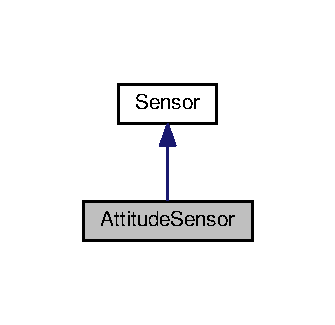
\includegraphics[width=161pt]{classAttitudeSensor__inherit__graph}
\end{center}
\end{figure}


Collaboration diagram for Attitude\+Sensor\+:\nopagebreak
\begin{figure}[H]
\begin{center}
\leavevmode
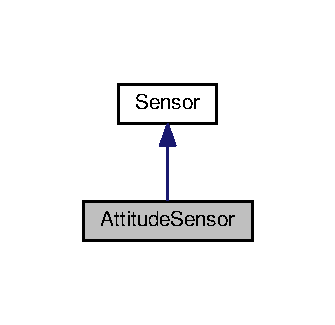
\includegraphics[width=161pt]{classAttitudeSensor__coll__graph}
\end{center}
\end{figure}
\subsection*{Public Member Functions}
\begin{DoxyCompactItemize}
\item 
\hyperlink{classAttitudeSensor_ada1382f003b390e357e9617e00299ddd}{Attitude\+Sensor} (int sensor\+Handle)
\begin{DoxyCompactList}\small\item\em Basic constructor. \end{DoxyCompactList}\item 
void \hyperlink{classAttitudeSensor_a5015e591534c5e80bd6646cc4719b417}{update} (std\+::vector$<$ float $>$ \&detect\+Point, int \&detect\+Handle, std\+::vector$<$ float $>$ \&detect\+Surface)
\begin{DoxyCompactList}\small\item\em Updates the sensor information, including any detected object information. \end{DoxyCompactList}\item 
int \hyperlink{classAttitudeSensor_a29d069767d7b3b36a998ae70764134dd}{get} (std\+::vector$<$ float $>$ \&detect\+Point, int \&detect\+Handle, std\+::vector$<$ float $>$ \&detect\+Surface)
\begin{DoxyCompactList}\small\item\em Retrieves the sensor information, including any detected object information. \end{DoxyCompactList}\end{DoxyCompactItemize}
\subsection*{Additional Inherited Members}


\subsection{Detailed Description}
Currently unused class for an attitude sensor. 

Implementation of an attitudesensor.

\begin{DoxyRefDesc}{Todo}
\item[\hyperlink{todo__todo000001}{Todo}]implement and use this for attitude calculation. \end{DoxyRefDesc}


\begin{DoxyRefDesc}{Todo}
\item[\hyperlink{todo__todo000002}{Todo}]actually use this for attitude calculation, implement noise. \end{DoxyRefDesc}


\subsection{Constructor \& Destructor Documentation}
\index{Attitude\+Sensor@{Attitude\+Sensor}!Attitude\+Sensor@{Attitude\+Sensor}}
\index{Attitude\+Sensor@{Attitude\+Sensor}!Attitude\+Sensor@{Attitude\+Sensor}}
\subsubsection[{\texorpdfstring{Attitude\+Sensor(int sensor\+Handle)}{AttitudeSensor(int sensorHandle)}}]{\setlength{\rightskip}{0pt plus 5cm}Attitude\+Sensor\+::\+Attitude\+Sensor (
\begin{DoxyParamCaption}
\item[{int}]{sensor\+Handle}
\end{DoxyParamCaption}
)}\hypertarget{classAttitudeSensor_ada1382f003b390e357e9617e00299ddd}{}\label{classAttitudeSensor_ada1382f003b390e357e9617e00299ddd}


Basic constructor. 


\begin{DoxyParams}{Parameters}
{\em sensor\+Handle} & The handle of the sensor in V-\/\+R\+EP \\
\hline
\end{DoxyParams}


\subsection{Member Function Documentation}
\index{Attitude\+Sensor@{Attitude\+Sensor}!get@{get}}
\index{get@{get}!Attitude\+Sensor@{Attitude\+Sensor}}
\subsubsection[{\texorpdfstring{get(std\+::vector$<$ float $>$ \&detect\+Point, int \&detect\+Handle, std\+::vector$<$ float $>$ \&detect\+Surface)}{get(std::vector< float > &detectPoint, int &detectHandle, std::vector< float > &detectSurface)}}]{\setlength{\rightskip}{0pt plus 5cm}int Attitude\+Sensor\+::get (
\begin{DoxyParamCaption}
\item[{std\+::vector$<$ float $>$ \&}]{detect\+Point, }
\item[{int \&}]{detect\+Handle, }
\item[{std\+::vector$<$ float $>$ \&}]{detect\+Surface}
\end{DoxyParamCaption}
)\hspace{0.3cm}{\ttfamily [virtual]}}\hypertarget{classAttitudeSensor_a29d069767d7b3b36a998ae70764134dd}{}\label{classAttitudeSensor_a29d069767d7b3b36a998ae70764134dd}


Retrieves the sensor information, including any detected object information. 


\begin{DoxyParams}{Parameters}
{\em detect\+Point} & Coordinates of the closest detected point. \\
\hline
{\em detect\+Handle} & The handle of the detected object. \\
\hline
{\em detect\+Surface} & Normal vector of the detected surface.\\
\hline
\end{DoxyParams}
\begin{DoxyReturn}{Returns}
0 or 1, depending on the detection state of the sensor and -\/1 in case of any error. See the \href{http://www.coppeliarobotics.com/helpFiles/en/regularApi/simHandleProximitySensor.htm}{\tt V-\/\+R\+EP A\+PI} for more info. 
\end{DoxyReturn}


Implements \hyperlink{classSensor_a997a8679d48c4fa346e6ac43c1e6219a}{Sensor}.

\index{Attitude\+Sensor@{Attitude\+Sensor}!update@{update}}
\index{update@{update}!Attitude\+Sensor@{Attitude\+Sensor}}
\subsubsection[{\texorpdfstring{update(std\+::vector$<$ float $>$ \&detect\+Point, int \&detect\+Handle, std\+::vector$<$ float $>$ \&detect\+Surface)}{update(std::vector< float > &detectPoint, int &detectHandle, std::vector< float > &detectSurface)}}]{\setlength{\rightskip}{0pt plus 5cm}void Attitude\+Sensor\+::update (
\begin{DoxyParamCaption}
\item[{std\+::vector$<$ float $>$ \&}]{detect\+Point, }
\item[{int \&}]{detect\+Handle, }
\item[{std\+::vector$<$ float $>$ \&}]{detect\+Surface}
\end{DoxyParamCaption}
)\hspace{0.3cm}{\ttfamily [virtual]}}\hypertarget{classAttitudeSensor_a5015e591534c5e80bd6646cc4719b417}{}\label{classAttitudeSensor_a5015e591534c5e80bd6646cc4719b417}


Updates the sensor information, including any detected object information. 


\begin{DoxyParams}{Parameters}
{\em detect\+Point} & Coordinates of the closest detected point. \\
\hline
{\em detect\+Handle} & The handle of the detected object. \\
\hline
{\em detect\+Surface} & Normal vector of the detected surface.\\
\hline
\end{DoxyParams}
See the \href{http://www.coppeliarobotics.com/helpFiles/en/regularApi/simReadProximitySensor.htm}{\tt V-\/\+R\+EP A\+PI} for more info. 

Implements \hyperlink{classSensor_aae4a856357eba6f54139b5add751d230}{Sensor}.



The documentation for this class was generated from the following files\+:\begin{DoxyCompactItemize}
\item 
\hyperlink{attitudesensor_8h}{attitudesensor.\+h}\item 
\hyperlink{attitudesensor_8cpp}{attitudesensor.\+cpp}\end{DoxyCompactItemize}

\hypertarget{classFinken}{}\section{Finken Class Reference}
\label{classFinken}\index{Finken@{Finken}}


implementation of a \hyperlink{classFinken}{Finken} rotorcraft, includes communication loop  




{\ttfamily \#include $<$finken.\+h$>$}

\subsection*{Public Member Functions}
\begin{DoxyCompactItemize}
\item 
\hyperlink{classFinken_afb256567ee9aa96c409fdb0529b4f228}{Finken} ()
\item 
\hyperlink{classFinken_a26a9cd42385ec3ae010e2ad1387d9ce6}{Finken} (int f\+Handle, int \+\_\+ac\+\_\+id, int \hyperlink{classFinken_a2de6be70e0baaf63641df0214bf1f7a2}{rotor\+Count}, int \hyperlink{classFinken_a92ae4d32222c44c17a4cea91055569d9}{sonar\+Count})
\item 
\hyperlink{classFinken_a94e6a3b5b14ec7ee351d219eb17be45b}{$\sim$\+Finken} ()
\item 
void \hyperlink{classFinken_aa4779668e3bf85253e371b30e0da808a}{connect} (std\+::unique\+\_\+ptr$<$ tcp\+::iostream $>$ \&\&s\+Ptr)
\item 
void \hyperlink{classFinken_ae3c3abbf571407e210f4b03b68cada9d}{run} (std\+::unique\+\_\+ptr$<$ tcp\+::iostream $>$ s\+Ptr)
\item 
void \hyperlink{classFinken_aaead1098c0752c8ec5b99bccd9945f3b}{set\+Rotor\+Speeds} ()
\item 
void \hyperlink{classFinken_afddc56af42f000ff17c4a00779b4ad6a}{update\+Pos} (\hyperlink{classFinken}{Finken} \&finken)
\item 
std\+::vector$<$ std\+::unique\+\_\+ptr$<$ \hyperlink{classSensor}{Sensor} $>$ $>$ \& \hyperlink{classFinken_a1215883fb6df7c4853e498dec43b4e6a}{get\+Sensors} ()
\item 
std\+::vector$<$ std\+::unique\+\_\+ptr$<$ \hyperlink{classRotor}{Rotor} $>$ $>$ \& \hyperlink{classFinken_a610ce496f1c5f2ca22850ee26c54510c}{get\+Rotors} ()
\end{DoxyCompactItemize}
\begin{Indent}{\bf Construction functions}\par
{\em Functions needed to construct the copter in the vrep plugin \begin{DoxySeeAlso}{See also}
\hyperlink{finken_8cpp_ab8920c514423348469521fe0063534c4}{build\+Finken()} 
\end{DoxySeeAlso}
}\begin{DoxyCompactItemize}
\item 
void \hyperlink{classFinken_a2f2adb211e80a689f580b87730aeb9d1}{add\+Sensor} (std\+::unique\+\_\+ptr$<$ \hyperlink{classSensor}{Sensor} $>$ \&sensor)
\item 
void \hyperlink{classFinken_a4ac9d9b37fba41147a83a36286fbe91b}{add\+Rotor} (std\+::unique\+\_\+ptr$<$ \hyperlink{classRotor}{Rotor} $>$ \&rotor)
\end{DoxyCompactItemize}
\end{Indent}
\subsection*{Public Attributes}
\begin{DoxyCompactItemize}
\item 
int \hyperlink{classFinken_a96990553bc26c8bf26effe8edd6e6369}{handle}
\item 
int \hyperlink{classFinken_aef4736605ea21831e5340f66a931f8ac}{base\+Handle}
\item 
const int \hyperlink{classFinken_a496f5024f0876710ca1cfd55a2924e85}{ac\+\_\+id}
\item 
const int \hyperlink{classFinken_a2de6be70e0baaf63641df0214bf1f7a2}{rotor\+Count}
\item 
const int \hyperlink{classFinken_a92ae4d32222c44c17a4cea91055569d9}{sonar\+Count}
\item 
bool \hyperlink{classFinken_a83131e08852cbcebaffa1eef80164a6e}{connected} = 0
\item 
std\+::thread {\bfseries run\+Thread}\hypertarget{classFinken_a490f025c596b5c87d1c583124b53e34b}{}\label{classFinken_a490f025c596b5c87d1c583124b53e34b}

\item 
std\+::vector$<$ double $>$ \hyperlink{classFinken_aa4fe546d88b52ff92990bd67ced70567}{commands} = \{0,0,0,0\}
\end{DoxyCompactItemize}
\begin{Indent}{\bf Copter state}\par
{\em \label{classFinken_copterstate}%
\hypertarget{classFinken_copterstate}{}%
 Members representing the current copter state }\begin{DoxyCompactItemize}
\item 
std\+::vector$<$ double $>$ \hyperlink{classFinken_a726c0ea1d756fe0837a3f042665d8d4a}{pos} = \{-\/1,-\/1,-\/1\}
\item 
std\+::vector$<$ double $>$ \hyperlink{classFinken_a3968cbe3b6f76678367ecb61f044a221}{quat} = \{-\/1,-\/1,-\/1,-\/1\}
\item 
std\+::vector$<$ double $>$ \hyperlink{classFinken_a4dd260e6384e7cfb8040bd53fe1c2d62}{vel} = \{-\/1,-\/1,-\/1\}
\item 
std\+::vector$<$ double $>$ \hyperlink{classFinken_a518ab8ab8ac8cf54c0b79cbc1ec2075f}{rot\+Vel} =\{-\/1,-\/1,-\/1\}
\item 
std\+::vector$<$ double $>$ \hyperlink{classFinken_a6f9723479baee5573447036270a2a722}{accel} = \{-\/1,-\/1,-\/1\}
\item 
std\+::vector$<$ double $>$ \hyperlink{classFinken_ab1b738a1b691879be240b1b9488f7009}{rot\+Accel} =\{-\/1,-\/1,-\/1\}
\end{DoxyCompactItemize}
\end{Indent}


\subsection{Detailed Description}
implementation of a \hyperlink{classFinken}{Finken} rotorcraft, includes communication loop 

\hyperlink{classFinken}{Finken} class for handling any data exchanges between a F\+I\+Nken and paparazzi. Also handles the application of rotor mixing commands to the F\+I\+Nken. 

\subsection{Constructor \& Destructor Documentation}
\index{Finken@{Finken}!Finken@{Finken}}
\index{Finken@{Finken}!Finken@{Finken}}
\subsubsection[{\texorpdfstring{Finken()}{Finken()}}]{\setlength{\rightskip}{0pt plus 5cm}Finken\+::\+Finken (
\begin{DoxyParamCaption}
{}
\end{DoxyParamCaption}
)}\hypertarget{classFinken_afb256567ee9aa96c409fdb0529b4f228}{}\label{classFinken_afb256567ee9aa96c409fdb0529b4f228}
Basic Empty Constructor \index{Finken@{Finken}!Finken@{Finken}}
\index{Finken@{Finken}!Finken@{Finken}}
\subsubsection[{\texorpdfstring{Finken(int f\+Handle, int \+\_\+ac\+\_\+id, int rotor\+Count, int sonar\+Count)}{Finken(int fHandle, int _ac_id, int rotorCount, int sonarCount)}}]{\setlength{\rightskip}{0pt plus 5cm}Finken\+::\+Finken (
\begin{DoxyParamCaption}
\item[{int}]{f\+Handle, }
\item[{int}]{\+\_\+ac\+\_\+id, }
\item[{int}]{rotor\+Count, }
\item[{int}]{sonar\+Count}
\end{DoxyParamCaption}
)}\hypertarget{classFinken_a26a9cd42385ec3ae010e2ad1387d9ce6}{}\label{classFinken_a26a9cd42385ec3ae010e2ad1387d9ce6}
Constructor for creating a uniquely identifiable finken 
\begin{DoxyParams}{Parameters}
{\em f\+Handle} & the handle used to identify the finken in vrep \\
\hline
{\em \+\_\+ac\+\_\+id} & the Aircraft ID used to identify the copter in paparazzi \\
\hline
\end{DoxyParams}
\index{Finken@{Finken}!````~Finken@{$\sim$\+Finken}}
\index{````~Finken@{$\sim$\+Finken}!Finken@{Finken}}
\subsubsection[{\texorpdfstring{$\sim$\+Finken()}{~Finken()}}]{\setlength{\rightskip}{0pt plus 5cm}Finken\+::$\sim$\+Finken (
\begin{DoxyParamCaption}
{}
\end{DoxyParamCaption}
)\hspace{0.3cm}{\ttfamily [inline]}}\hypertarget{classFinken_a94e6a3b5b14ec7ee351d219eb17be45b}{}\label{classFinken_a94e6a3b5b14ec7ee351d219eb17be45b}
Basic destructor 

\subsection{Member Function Documentation}
\index{Finken@{Finken}!add\+Rotor@{add\+Rotor}}
\index{add\+Rotor@{add\+Rotor}!Finken@{Finken}}
\subsubsection[{\texorpdfstring{add\+Rotor(std\+::unique\+\_\+ptr$<$ Rotor $>$ \&rotor)}{addRotor(std::unique_ptr< Rotor > &rotor)}}]{\setlength{\rightskip}{0pt plus 5cm}void Finken\+::add\+Rotor (
\begin{DoxyParamCaption}
\item[{std\+::unique\+\_\+ptr$<$ {\bf Rotor} $>$ \&}]{rotor}
\end{DoxyParamCaption}
)}\hypertarget{classFinken_a4ac9d9b37fba41147a83a36286fbe91b}{}\label{classFinken_a4ac9d9b37fba41147a83a36286fbe91b}
Adding rotors to the copter. \index{Finken@{Finken}!add\+Sensor@{add\+Sensor}}
\index{add\+Sensor@{add\+Sensor}!Finken@{Finken}}
\subsubsection[{\texorpdfstring{add\+Sensor(std\+::unique\+\_\+ptr$<$ Sensor $>$ \&sensor)}{addSensor(std::unique_ptr< Sensor > &sensor)}}]{\setlength{\rightskip}{0pt plus 5cm}void Finken\+::add\+Sensor (
\begin{DoxyParamCaption}
\item[{std\+::unique\+\_\+ptr$<$ {\bf Sensor} $>$ \&}]{sensor}
\end{DoxyParamCaption}
)}\hypertarget{classFinken_a2f2adb211e80a689f580b87730aeb9d1}{}\label{classFinken_a2f2adb211e80a689f580b87730aeb9d1}
Adding sensors to the copter. \index{Finken@{Finken}!connect@{connect}}
\index{connect@{connect}!Finken@{Finken}}
\subsubsection[{\texorpdfstring{connect(std\+::unique\+\_\+ptr$<$ tcp\+::iostream $>$ \&\&s\+Ptr)}{connect(std::unique_ptr< tcp::iostream > &&sPtr)}}]{\setlength{\rightskip}{0pt plus 5cm}void Finken\+::connect (
\begin{DoxyParamCaption}
\item[{std\+::unique\+\_\+ptr$<$ tcp\+::iostream $>$ \&\&}]{s\+Ptr}
\end{DoxyParamCaption}
)\hspace{0.3cm}{\ttfamily [inline]}}\hypertarget{classFinken_aa4779668e3bf85253e371b30e0da808a}{}\label{classFinken_aa4779668e3bf85253e371b30e0da808a}
Called in the accept handler, this function passes the incoming connection to the corresponding finken in a new thread \index{Finken@{Finken}!get\+Rotors@{get\+Rotors}}
\index{get\+Rotors@{get\+Rotors}!Finken@{Finken}}
\subsubsection[{\texorpdfstring{get\+Rotors()}{getRotors()}}]{\setlength{\rightskip}{0pt plus 5cm}std\+::vector$<$ std\+::unique\+\_\+ptr$<$ {\bf Rotor} $>$ $>$ \& Finken\+::get\+Rotors (
\begin{DoxyParamCaption}
{}
\end{DoxyParamCaption}
)}\hypertarget{classFinken_a610ce496f1c5f2ca22850ee26c54510c}{}\label{classFinken_a610ce496f1c5f2ca22850ee26c54510c}
returns a vector containing all rotors of the finken \index{Finken@{Finken}!get\+Sensors@{get\+Sensors}}
\index{get\+Sensors@{get\+Sensors}!Finken@{Finken}}
\subsubsection[{\texorpdfstring{get\+Sensors()}{getSensors()}}]{\setlength{\rightskip}{0pt plus 5cm}std\+::vector$<$ std\+::unique\+\_\+ptr$<$ {\bf Sensor} $>$ $>$ \& Finken\+::get\+Sensors (
\begin{DoxyParamCaption}
{}
\end{DoxyParamCaption}
)}\hypertarget{classFinken_a1215883fb6df7c4853e498dec43b4e6a}{}\label{classFinken_a1215883fb6df7c4853e498dec43b4e6a}
returns a vector containing all sensors of the finken \index{Finken@{Finken}!run@{run}}
\index{run@{run}!Finken@{Finken}}
\subsubsection[{\texorpdfstring{run(std\+::unique\+\_\+ptr$<$ tcp\+::iostream $>$ s\+Ptr)}{run(std::unique_ptr< tcp::iostream > sPtr)}}]{\setlength{\rightskip}{0pt plus 5cm}void Finken\+::run (
\begin{DoxyParamCaption}
\item[{std\+::unique\+\_\+ptr$<$ tcp\+::iostream $>$}]{s\+Ptr}
\end{DoxyParamCaption}
)}\hypertarget{classFinken_ae3c3abbf571407e210f4b03b68cada9d}{}\label{classFinken_ae3c3abbf571407e210f4b03b68cada9d}
Main function containing the paparazzi-\/vrep communication loop. Called whenever a new connection from paparazzi to the vrep server is established, see Async\+\_\+\+Server\+::handle\+\_\+accept() 
\begin{DoxyParams}{Parameters}
{\em s\+Ptr} & the iostream of the connection \\
\hline
\end{DoxyParams}
\begin{DoxySeeAlso}{See also}
Async\+\_\+\+Server\+::handle\+\_\+accept() 
\end{DoxySeeAlso}
\index{Finken@{Finken}!set\+Rotor\+Speeds@{set\+Rotor\+Speeds}}
\index{set\+Rotor\+Speeds@{set\+Rotor\+Speeds}!Finken@{Finken}}
\subsubsection[{\texorpdfstring{set\+Rotor\+Speeds()}{setRotorSpeeds()}}]{\setlength{\rightskip}{0pt plus 5cm}void Finken\+::set\+Rotor\+Speeds (
\begin{DoxyParamCaption}
{}
\end{DoxyParamCaption}
)}\hypertarget{classFinken_aaead1098c0752c8ec5b99bccd9945f3b}{}\label{classFinken_aaead1098c0752c8ec5b99bccd9945f3b}
Applies the correct rotor speeds calculated by paparazzi \begin{DoxySeeAlso}{See also}
\hyperlink{classFinken_aa4fe546d88b52ff92990bd67ced70567}{Finken\+::commands} 

\hyperlink{finken_8h_a4e838d73ad5e098825ef4c227f6369b6}{thrust\+From\+Throttle} 
\end{DoxySeeAlso}
\index{Finken@{Finken}!update\+Pos@{update\+Pos}}
\index{update\+Pos@{update\+Pos}!Finken@{Finken}}
\subsubsection[{\texorpdfstring{update\+Pos(\+Finken \&finken)}{updatePos(Finken &finken)}}]{\setlength{\rightskip}{0pt plus 5cm}void Finken\+::update\+Pos (
\begin{DoxyParamCaption}
\item[{{\bf Finken} \&}]{finken}
\end{DoxyParamCaption}
)}\hypertarget{classFinken_afddc56af42f000ff17c4a00779b4ad6a}{}\label{classFinken_afddc56af42f000ff17c4a00779b4ad6a}
updates the values for copter position and attitude, namely the \hyperlink{classFinken_copterstate}{copter state} vectors 
\begin{DoxyParams}{Parameters}
{\em finken} & reference to the finken to be updated \\
\hline
\end{DoxyParams}


\subsection{Member Data Documentation}
\index{Finken@{Finken}!ac\+\_\+id@{ac\+\_\+id}}
\index{ac\+\_\+id@{ac\+\_\+id}!Finken@{Finken}}
\subsubsection[{\texorpdfstring{ac\+\_\+id}{ac_id}}]{\setlength{\rightskip}{0pt plus 5cm}const int Finken\+::ac\+\_\+id}\hypertarget{classFinken_a496f5024f0876710ca1cfd55a2924e85}{}\label{classFinken_a496f5024f0876710ca1cfd55a2924e85}
Integer representing the Aircraft ID to match copters in vrep and paparazzi \index{Finken@{Finken}!accel@{accel}}
\index{accel@{accel}!Finken@{Finken}}
\subsubsection[{\texorpdfstring{accel}{accel}}]{\setlength{\rightskip}{0pt plus 5cm}std\+::vector$<$double$>$ Finken\+::accel = \{-\/1,-\/1,-\/1\}}\hypertarget{classFinken_a6f9723479baee5573447036270a2a722}{}\label{classFinken_a6f9723479baee5573447036270a2a722}
Copter acceleration \index{Finken@{Finken}!base\+Handle@{base\+Handle}}
\index{base\+Handle@{base\+Handle}!Finken@{Finken}}
\subsubsection[{\texorpdfstring{base\+Handle}{baseHandle}}]{\setlength{\rightskip}{0pt plus 5cm}int Finken\+::base\+Handle}\hypertarget{classFinken_aef4736605ea21831e5340f66a931f8ac}{}\label{classFinken_aef4736605ea21831e5340f66a931f8ac}
Integer representing the handle of the copter base in Vrep. Copter base, not the copter object is used for the calculation of the copter state. \index{Finken@{Finken}!commands@{commands}}
\index{commands@{commands}!Finken@{Finken}}
\subsubsection[{\texorpdfstring{commands}{commands}}]{\setlength{\rightskip}{0pt plus 5cm}std\+::vector$<$double$>$ Finken\+::commands = \{0,0,0,0\}}\hypertarget{classFinken_aa4fe546d88b52ff92990bd67ced70567}{}\label{classFinken_aa4fe546d88b52ff92990bd67ced70567}
Vector storing the commands provided by paparazzi \index{Finken@{Finken}!connected@{connected}}
\index{connected@{connected}!Finken@{Finken}}
\subsubsection[{\texorpdfstring{connected}{connected}}]{\setlength{\rightskip}{0pt plus 5cm}bool Finken\+::connected = 0}\hypertarget{classFinken_a83131e08852cbcebaffa1eef80164a6e}{}\label{classFinken_a83131e08852cbcebaffa1eef80164a6e}
current connection status of the copter \index{Finken@{Finken}!handle@{handle}}
\index{handle@{handle}!Finken@{Finken}}
\subsubsection[{\texorpdfstring{handle}{handle}}]{\setlength{\rightskip}{0pt plus 5cm}int Finken\+::handle}\hypertarget{classFinken_a96990553bc26c8bf26effe8edd6e6369}{}\label{classFinken_a96990553bc26c8bf26effe8edd6e6369}
Integer representing the handle of the copter object in vrep \index{Finken@{Finken}!pos@{pos}}
\index{pos@{pos}!Finken@{Finken}}
\subsubsection[{\texorpdfstring{pos}{pos}}]{\setlength{\rightskip}{0pt plus 5cm}std\+::vector$<$double$>$ Finken\+::pos = \{-\/1,-\/1,-\/1\}}\hypertarget{classFinken_a726c0ea1d756fe0837a3f042665d8d4a}{}\label{classFinken_a726c0ea1d756fe0837a3f042665d8d4a}
Copter position (E\+NU) \index{Finken@{Finken}!quat@{quat}}
\index{quat@{quat}!Finken@{Finken}}
\subsubsection[{\texorpdfstring{quat}{quat}}]{\setlength{\rightskip}{0pt plus 5cm}std\+::vector$<$double$>$ Finken\+::quat = \{-\/1,-\/1,-\/1,-\/1\}}\hypertarget{classFinken_a3968cbe3b6f76678367ecb61f044a221}{}\label{classFinken_a3968cbe3b6f76678367ecb61f044a221}
Copter Quaternion \index{Finken@{Finken}!rot\+Accel@{rot\+Accel}}
\index{rot\+Accel@{rot\+Accel}!Finken@{Finken}}
\subsubsection[{\texorpdfstring{rot\+Accel}{rotAccel}}]{\setlength{\rightskip}{0pt plus 5cm}std\+::vector$<$double$>$ Finken\+::rot\+Accel =\{-\/1,-\/1,-\/1\}}\hypertarget{classFinken_ab1b738a1b691879be240b1b9488f7009}{}\label{classFinken_ab1b738a1b691879be240b1b9488f7009}
Copter rotational acceleration (aka angular acceleration) \index{Finken@{Finken}!rotor\+Count@{rotor\+Count}}
\index{rotor\+Count@{rotor\+Count}!Finken@{Finken}}
\subsubsection[{\texorpdfstring{rotor\+Count}{rotorCount}}]{\setlength{\rightskip}{0pt plus 5cm}const int Finken\+::rotor\+Count}\hypertarget{classFinken_a2de6be70e0baaf63641df0214bf1f7a2}{}\label{classFinken_a2de6be70e0baaf63641df0214bf1f7a2}
Integer representing the amount of rotors, used in automatic finken construction \begin{DoxySeeAlso}{See also}
\hyperlink{finken_8cpp_ab8920c514423348469521fe0063534c4}{build\+Finken()} 
\end{DoxySeeAlso}
\index{Finken@{Finken}!rot\+Vel@{rot\+Vel}}
\index{rot\+Vel@{rot\+Vel}!Finken@{Finken}}
\subsubsection[{\texorpdfstring{rot\+Vel}{rotVel}}]{\setlength{\rightskip}{0pt plus 5cm}std\+::vector$<$double$>$ Finken\+::rot\+Vel =\{-\/1,-\/1,-\/1\}}\hypertarget{classFinken_a518ab8ab8ac8cf54c0b79cbc1ec2075f}{}\label{classFinken_a518ab8ab8ac8cf54c0b79cbc1ec2075f}
Copter rotational velocity (aka angular velocity) \index{Finken@{Finken}!sonar\+Count@{sonar\+Count}}
\index{sonar\+Count@{sonar\+Count}!Finken@{Finken}}
\subsubsection[{\texorpdfstring{sonar\+Count}{sonarCount}}]{\setlength{\rightskip}{0pt plus 5cm}const int Finken\+::sonar\+Count}\hypertarget{classFinken_a92ae4d32222c44c17a4cea91055569d9}{}\label{classFinken_a92ae4d32222c44c17a4cea91055569d9}
Integer representing the amount of sonars, used in automatic finken construction$\ast$$\ast$ \begin{DoxySeeAlso}{See also}
\hyperlink{finken_8h_ab8920c514423348469521fe0063534c4}{build\+Finken} / 
\end{DoxySeeAlso}
\index{Finken@{Finken}!vel@{vel}}
\index{vel@{vel}!Finken@{Finken}}
\subsubsection[{\texorpdfstring{vel}{vel}}]{\setlength{\rightskip}{0pt plus 5cm}std\+::vector$<$double$>$ Finken\+::vel = \{-\/1,-\/1,-\/1\}}\hypertarget{classFinken_a4dd260e6384e7cfb8040bd53fe1c2d62}{}\label{classFinken_a4dd260e6384e7cfb8040bd53fe1c2d62}
Copter velocity 

The documentation for this class was generated from the following files\+:\begin{DoxyCompactItemize}
\item 
\hyperlink{finken_8h}{finken.\+h}\item 
\hyperlink{finken_8cpp}{finken.\+cpp}\end{DoxyCompactItemize}

\hypertarget{classFinkenPlugin}{}\section{Finken\+Plugin Class Reference}
\label{classFinkenPlugin}\index{Finken\+Plugin@{Finken\+Plugin}}


The actual finken plugin.  




Inheritance diagram for Finken\+Plugin\+:\nopagebreak
\begin{figure}[H]
\begin{center}
\leavevmode
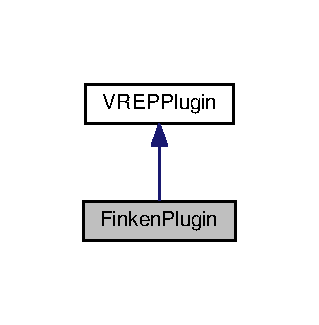
\includegraphics[width=153pt]{classFinkenPlugin__inherit__graph}
\end{center}
\end{figure}


Collaboration diagram for Finken\+Plugin\+:\nopagebreak
\begin{figure}[H]
\begin{center}
\leavevmode
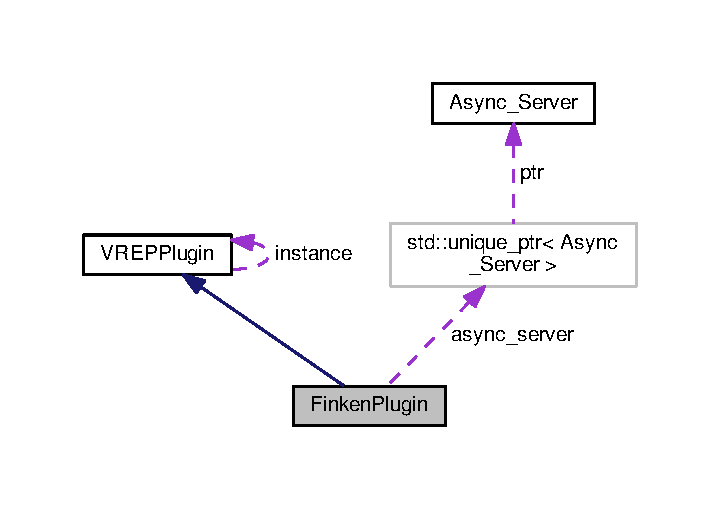
\includegraphics[width=346pt]{classFinkenPlugin__coll__graph}
\end{center}
\end{figure}
\subsection*{Public Member Functions}
\begin{DoxyCompactItemize}
\item 
\hyperlink{classFinkenPlugin_a03dadda0b43081bce8e8db1223289fe1}{Finken\+Plugin} ()
\begin{DoxyCompactList}\small\item\em Empty constructor. \end{DoxyCompactList}\item 
\hyperlink{classFinkenPlugin}{Finken\+Plugin} \& \hyperlink{classFinkenPlugin_a3ebea1e19535491b5db16c7f43df8e79}{operator=} (const \hyperlink{classFinkenPlugin}{Finken\+Plugin} \&)=delete
\begin{DoxyCompactList}\small\item\em No copying the Finkenplugin. \end{DoxyCompactList}\item 
\hyperlink{classFinkenPlugin_a5f4bc33c0d0bb05ca4f78090c7a2fda9}{Finken\+Plugin} (const \hyperlink{classFinkenPlugin}{Finken\+Plugin} \&)=delete
\begin{DoxyCompactList}\small\item\em No copying the Finkenplugin. \end{DoxyCompactList}\item 
virtual \hyperlink{classFinkenPlugin_acb58d49ecbfaaffd014ddeb80606dc52}{$\sim$\+Finken\+Plugin} ()
\begin{DoxyCompactList}\small\item\em Destructor. \end{DoxyCompactList}\item 
virtual unsigned char \hyperlink{classFinkenPlugin_a046a229dfbc8185bac916ad2e49ec865}{version} () const 
\item 
virtual bool \hyperlink{classFinkenPlugin_afbe5d82635afe4b0c407de4724e8ee14}{load} ()
\begin{DoxyCompactList}\small\item\em Loads the plugin into V-\/\+R\+EP. \end{DoxyCompactList}\item 
virtual bool \hyperlink{classFinkenPlugin_ae9c984b362c6a828206fa6201291851c}{unload} ()
\begin{DoxyCompactList}\small\item\em unloads the plugin \end{DoxyCompactList}\item 
virtual const std\+::string \hyperlink{classFinkenPlugin_a1a7d0d65f88654c37b282e07d36417ec}{name} () const 
\begin{DoxyCompactList}\small\item\em Function returning the name of the plugin . \end{DoxyCompactList}\item 
void $\ast$ \hyperlink{classFinkenPlugin_a82c0cd5fa1b9fdb5f5a625458a9b545b}{scene\+Load} (int $\ast$auxiliary\+Data, void $\ast$custom\+Data, int $\ast$reply\+Data)
\begin{DoxyCompactList}\small\item\em Called once on the loading of any scene, it checks for the presence of a Dummy object \char`\"{}\+Script\+Loader\char`\"{} in the scene. \end{DoxyCompactList}\item 
void $\ast$ \hyperlink{classFinkenPlugin_a142f62305fcc926bb6cf86744edbb82b}{sim\+Start} (int $\ast$auxiliary\+Data, void $\ast$custom\+Data, int $\ast$reply\+Data)
\begin{DoxyCompactList}\small\item\em Called when the Simulation is started. \end{DoxyCompactList}\item 
void $\ast$ \hyperlink{classFinkenPlugin_aec5f5cf14ca485055ccc321a716780a4}{sim\+End} (int $\ast$auxiliary\+Data, void $\ast$custom\+Data, int $\ast$reply\+Data)
\begin{DoxyCompactList}\small\item\em Ends the simulation run and cleans up the server and F\+I\+Nken. \end{DoxyCompactList}\item 
void $\ast$ \hyperlink{classFinkenPlugin_a00d8bcdd7c4b28eb76712b84f512b12b}{action} (int $\ast$auxiliary\+Data, void $\ast$custom\+Data, int $\ast$reply\+Data)
\begin{DoxyCompactList}\small\item\em This function controls the other parts of the plugin and synchronizes the vrep copters with the paparazzi copters. \end{DoxyCompactList}\end{DoxyCompactItemize}
\subsection*{Public Attributes}
\begin{DoxyCompactItemize}
\item 
boost\+::asio\+::io\+\_\+service \hyperlink{classFinkenPlugin_a895a0de924a1c60e3cb65ff1cf139fdc}{io\+\_\+service}
\begin{DoxyCompactList}\small\item\em The io service for the server. \end{DoxyCompactList}\item 
std\+::unique\+\_\+ptr$<$ \hyperlink{classAsync__Server}{Async\+\_\+\+Server} $>$ \hyperlink{classFinkenPlugin_aeb198541b548eb5b1ba09221aaa35a26}{async\+\_\+server}
\begin{DoxyCompactList}\small\item\em Pointer to the server responsible for communication with Paparazzi. \end{DoxyCompactList}\end{DoxyCompactItemize}
\subsection*{Additional Inherited Members}


\subsection{Detailed Description}
The actual finken plugin. 

Implementation of the baseline functionality for the plugin and the communication with Paparazzi.

This class handles the main communication with vrep and calls for copter actions each timestep. It is also responsible for starting the server to communicate with paparazzi.

\begin{DoxyRefDesc}{Todo}
\item[\hyperlink{todo__todo000005}{Todo}]This could use a .h file. \end{DoxyRefDesc}


\subsection{Constructor \& Destructor Documentation}
\index{Finken\+Plugin@{Finken\+Plugin}!Finken\+Plugin@{Finken\+Plugin}}
\index{Finken\+Plugin@{Finken\+Plugin}!Finken\+Plugin@{Finken\+Plugin}}
\subsubsection[{\texorpdfstring{Finken\+Plugin()}{FinkenPlugin()}}]{\setlength{\rightskip}{0pt plus 5cm}Finken\+Plugin\+::\+Finken\+Plugin (
\begin{DoxyParamCaption}
{}
\end{DoxyParamCaption}
)\hspace{0.3cm}{\ttfamily [inline]}}\hypertarget{classFinkenPlugin_a03dadda0b43081bce8e8db1223289fe1}{}\label{classFinkenPlugin_a03dadda0b43081bce8e8db1223289fe1}


Empty constructor. 

\index{Finken\+Plugin@{Finken\+Plugin}!Finken\+Plugin@{Finken\+Plugin}}
\index{Finken\+Plugin@{Finken\+Plugin}!Finken\+Plugin@{Finken\+Plugin}}
\subsubsection[{\texorpdfstring{Finken\+Plugin(const Finken\+Plugin \&)=delete}{FinkenPlugin(const FinkenPlugin &)=delete}}]{\setlength{\rightskip}{0pt plus 5cm}Finken\+Plugin\+::\+Finken\+Plugin (
\begin{DoxyParamCaption}
\item[{const {\bf Finken\+Plugin} \&}]{}
\end{DoxyParamCaption}
)\hspace{0.3cm}{\ttfamily [delete]}}\hypertarget{classFinkenPlugin_a5f4bc33c0d0bb05ca4f78090c7a2fda9}{}\label{classFinkenPlugin_a5f4bc33c0d0bb05ca4f78090c7a2fda9}


No copying the Finkenplugin. 

\index{Finken\+Plugin@{Finken\+Plugin}!````~Finken\+Plugin@{$\sim$\+Finken\+Plugin}}
\index{````~Finken\+Plugin@{$\sim$\+Finken\+Plugin}!Finken\+Plugin@{Finken\+Plugin}}
\subsubsection[{\texorpdfstring{$\sim$\+Finken\+Plugin()}{~FinkenPlugin()}}]{\setlength{\rightskip}{0pt plus 5cm}virtual Finken\+Plugin\+::$\sim$\+Finken\+Plugin (
\begin{DoxyParamCaption}
{}
\end{DoxyParamCaption}
)\hspace{0.3cm}{\ttfamily [inline]}, {\ttfamily [virtual]}}\hypertarget{classFinkenPlugin_acb58d49ecbfaaffd014ddeb80606dc52}{}\label{classFinkenPlugin_acb58d49ecbfaaffd014ddeb80606dc52}


Destructor. 



\subsection{Member Function Documentation}
\index{Finken\+Plugin@{Finken\+Plugin}!action@{action}}
\index{action@{action}!Finken\+Plugin@{Finken\+Plugin}}
\subsubsection[{\texorpdfstring{action(int $\ast$auxiliary\+Data, void $\ast$custom\+Data, int $\ast$reply\+Data)}{action(int *auxiliaryData, void *customData, int *replyData)}}]{\setlength{\rightskip}{0pt plus 5cm}void$\ast$ Finken\+Plugin\+::action (
\begin{DoxyParamCaption}
\item[{int $\ast$}]{auxiliary\+Data, }
\item[{void $\ast$}]{custom\+Data, }
\item[{int $\ast$}]{reply\+Data}
\end{DoxyParamCaption}
)\hspace{0.3cm}{\ttfamily [inline]}, {\ttfamily [virtual]}}\hypertarget{classFinkenPlugin_a00d8bcdd7c4b28eb76712b84f512b12b}{}\label{classFinkenPlugin_a00d8bcdd7c4b28eb76712b84f512b12b}


This function controls the other parts of the plugin and synchronizes the vrep copters with the paparazzi copters. 



Reimplemented from \hyperlink{classVREPPlugin_a048e1fbf7b4b5b7b96ea6ec132218e12}{V\+R\+E\+P\+Plugin}.

\index{Finken\+Plugin@{Finken\+Plugin}!load@{load}}
\index{load@{load}!Finken\+Plugin@{Finken\+Plugin}}
\subsubsection[{\texorpdfstring{load()}{load()}}]{\setlength{\rightskip}{0pt plus 5cm}virtual bool Finken\+Plugin\+::load (
\begin{DoxyParamCaption}
{}
\end{DoxyParamCaption}
)\hspace{0.3cm}{\ttfamily [inline]}, {\ttfamily [virtual]}}\hypertarget{classFinkenPlugin_afbe5d82635afe4b0c407de4724e8ee14}{}\label{classFinkenPlugin_afbe5d82635afe4b0c407de4724e8ee14}


Loads the plugin into V-\/\+R\+EP. 

\begin{DoxyReturn}{Returns}
true 
\end{DoxyReturn}


Reimplemented from \hyperlink{classVREPPlugin_a4149b72b671ad72f63e9a75c58c0d628}{V\+R\+E\+P\+Plugin}.



Here is the call graph for this function\+:\nopagebreak
\begin{figure}[H]
\begin{center}
\leavevmode
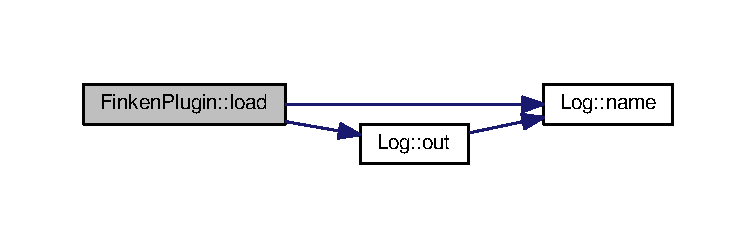
\includegraphics[width=350pt]{classFinkenPlugin_afbe5d82635afe4b0c407de4724e8ee14_cgraph}
\end{center}
\end{figure}


\index{Finken\+Plugin@{Finken\+Plugin}!name@{name}}
\index{name@{name}!Finken\+Plugin@{Finken\+Plugin}}
\subsubsection[{\texorpdfstring{name() const }{name() const }}]{\setlength{\rightskip}{0pt plus 5cm}virtual const std\+::string Finken\+Plugin\+::name (
\begin{DoxyParamCaption}
{}
\end{DoxyParamCaption}
) const\hspace{0.3cm}{\ttfamily [inline]}, {\ttfamily [virtual]}}\hypertarget{classFinkenPlugin_a1a7d0d65f88654c37b282e07d36417ec}{}\label{classFinkenPlugin_a1a7d0d65f88654c37b282e07d36417ec}


Function returning the name of the plugin . 

\begin{DoxyReturn}{Returns}
Name as a string. 
\end{DoxyReturn}


Implements \hyperlink{classVREPPlugin_a345987cf0e2e8aa3af817cc0213e5c7a}{V\+R\+E\+P\+Plugin}.

\index{Finken\+Plugin@{Finken\+Plugin}!operator=@{operator=}}
\index{operator=@{operator=}!Finken\+Plugin@{Finken\+Plugin}}
\subsubsection[{\texorpdfstring{operator=(const Finken\+Plugin \&)=delete}{operator=(const FinkenPlugin &)=delete}}]{\setlength{\rightskip}{0pt plus 5cm}{\bf Finken\+Plugin}\& Finken\+Plugin\+::operator= (
\begin{DoxyParamCaption}
\item[{const {\bf Finken\+Plugin} \&}]{}
\end{DoxyParamCaption}
)\hspace{0.3cm}{\ttfamily [delete]}}\hypertarget{classFinkenPlugin_a3ebea1e19535491b5db16c7f43df8e79}{}\label{classFinkenPlugin_a3ebea1e19535491b5db16c7f43df8e79}


No copying the Finkenplugin. 

\index{Finken\+Plugin@{Finken\+Plugin}!scene\+Load@{scene\+Load}}
\index{scene\+Load@{scene\+Load}!Finken\+Plugin@{Finken\+Plugin}}
\subsubsection[{\texorpdfstring{scene\+Load(int $\ast$auxiliary\+Data, void $\ast$custom\+Data, int $\ast$reply\+Data)}{sceneLoad(int *auxiliaryData, void *customData, int *replyData)}}]{\setlength{\rightskip}{0pt plus 5cm}void$\ast$ Finken\+Plugin\+::scene\+Load (
\begin{DoxyParamCaption}
\item[{int $\ast$}]{auxiliary\+Data, }
\item[{void $\ast$}]{custom\+Data, }
\item[{int $\ast$}]{reply\+Data}
\end{DoxyParamCaption}
)\hspace{0.3cm}{\ttfamily [inline]}, {\ttfamily [virtual]}}\hypertarget{classFinkenPlugin_a82c0cd5fa1b9fdb5f5a625458a9b545b}{}\label{classFinkenPlugin_a82c0cd5fa1b9fdb5f5a625458a9b545b}


Called once on the loading of any scene, it checks for the presence of a Dummy object \char`\"{}\+Script\+Loader\char`\"{} in the scene. 

Only if that object is found, the server is startet and full functionality established. 

Reimplemented from \hyperlink{classVREPPlugin_a77e10632cbc7ae0581a151daea83ab1f}{V\+R\+E\+P\+Plugin}.



Here is the call graph for this function\+:\nopagebreak
\begin{figure}[H]
\begin{center}
\leavevmode
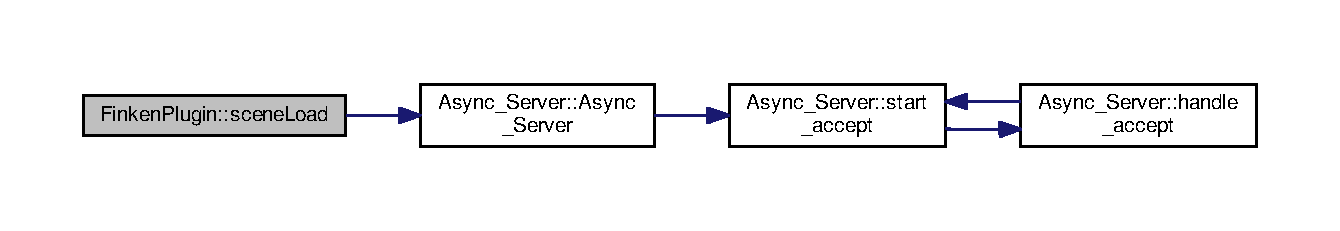
\includegraphics[width=350pt]{classFinkenPlugin_a82c0cd5fa1b9fdb5f5a625458a9b545b_cgraph}
\end{center}
\end{figure}


\index{Finken\+Plugin@{Finken\+Plugin}!sim\+End@{sim\+End}}
\index{sim\+End@{sim\+End}!Finken\+Plugin@{Finken\+Plugin}}
\subsubsection[{\texorpdfstring{sim\+End(int $\ast$auxiliary\+Data, void $\ast$custom\+Data, int $\ast$reply\+Data)}{simEnd(int *auxiliaryData, void *customData, int *replyData)}}]{\setlength{\rightskip}{0pt plus 5cm}void$\ast$ Finken\+Plugin\+::sim\+End (
\begin{DoxyParamCaption}
\item[{int $\ast$}]{auxiliary\+Data, }
\item[{void $\ast$}]{custom\+Data, }
\item[{int $\ast$}]{reply\+Data}
\end{DoxyParamCaption}
)\hspace{0.3cm}{\ttfamily [inline]}, {\ttfamily [virtual]}}\hypertarget{classFinkenPlugin_aec5f5cf14ca485055ccc321a716780a4}{}\label{classFinkenPlugin_aec5f5cf14ca485055ccc321a716780a4}


Ends the simulation run and cleans up the server and F\+I\+Nken. 



Reimplemented from \hyperlink{classVREPPlugin_a13ea56c8546d762468b21ebc141b4ca3}{V\+R\+E\+P\+Plugin}.

\index{Finken\+Plugin@{Finken\+Plugin}!sim\+Start@{sim\+Start}}
\index{sim\+Start@{sim\+Start}!Finken\+Plugin@{Finken\+Plugin}}
\subsubsection[{\texorpdfstring{sim\+Start(int $\ast$auxiliary\+Data, void $\ast$custom\+Data, int $\ast$reply\+Data)}{simStart(int *auxiliaryData, void *customData, int *replyData)}}]{\setlength{\rightskip}{0pt plus 5cm}void$\ast$ Finken\+Plugin\+::sim\+Start (
\begin{DoxyParamCaption}
\item[{int $\ast$}]{auxiliary\+Data, }
\item[{void $\ast$}]{custom\+Data, }
\item[{int $\ast$}]{reply\+Data}
\end{DoxyParamCaption}
)\hspace{0.3cm}{\ttfamily [inline]}, {\ttfamily [virtual]}}\hypertarget{classFinkenPlugin_a142f62305fcc926bb6cf86744edbb82b}{}\label{classFinkenPlugin_a142f62305fcc926bb6cf86744edbb82b}


Called when the Simulation is started. 



Reimplemented from \hyperlink{classVREPPlugin_a58c9675c38c6ca1a75047864d3e4253c}{V\+R\+E\+P\+Plugin}.

\index{Finken\+Plugin@{Finken\+Plugin}!unload@{unload}}
\index{unload@{unload}!Finken\+Plugin@{Finken\+Plugin}}
\subsubsection[{\texorpdfstring{unload()}{unload()}}]{\setlength{\rightskip}{0pt plus 5cm}virtual bool Finken\+Plugin\+::unload (
\begin{DoxyParamCaption}
{}
\end{DoxyParamCaption}
)\hspace{0.3cm}{\ttfamily [inline]}, {\ttfamily [virtual]}}\hypertarget{classFinkenPlugin_ae9c984b362c6a828206fa6201291851c}{}\label{classFinkenPlugin_ae9c984b362c6a828206fa6201291851c}


unloads the plugin 

\begin{DoxyReturn}{Returns}
true 
\end{DoxyReturn}


Reimplemented from \hyperlink{classVREPPlugin_a49aff8a71c1c9f2af6e32b918eba99ff}{V\+R\+E\+P\+Plugin}.



Here is the call graph for this function\+:\nopagebreak
\begin{figure}[H]
\begin{center}
\leavevmode
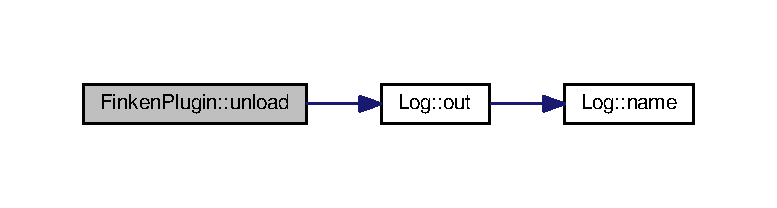
\includegraphics[width=350pt]{classFinkenPlugin_ae9c984b362c6a828206fa6201291851c_cgraph}
\end{center}
\end{figure}


\index{Finken\+Plugin@{Finken\+Plugin}!version@{version}}
\index{version@{version}!Finken\+Plugin@{Finken\+Plugin}}
\subsubsection[{\texorpdfstring{version() const }{version() const }}]{\setlength{\rightskip}{0pt plus 5cm}virtual unsigned char Finken\+Plugin\+::version (
\begin{DoxyParamCaption}
{}
\end{DoxyParamCaption}
) const\hspace{0.3cm}{\ttfamily [inline]}, {\ttfamily [virtual]}}\hypertarget{classFinkenPlugin_a046a229dfbc8185bac916ad2e49ec865}{}\label{classFinkenPlugin_a046a229dfbc8185bac916ad2e49ec865}


Implements \hyperlink{classVREPPlugin_ae5e6764e97874aa134447122bbadbf2a}{V\+R\+E\+P\+Plugin}.



\subsection{Member Data Documentation}
\index{Finken\+Plugin@{Finken\+Plugin}!async\+\_\+server@{async\+\_\+server}}
\index{async\+\_\+server@{async\+\_\+server}!Finken\+Plugin@{Finken\+Plugin}}
\subsubsection[{\texorpdfstring{async\+\_\+server}{async_server}}]{\setlength{\rightskip}{0pt plus 5cm}std\+::unique\+\_\+ptr$<${\bf Async\+\_\+\+Server}$>$ Finken\+Plugin\+::async\+\_\+server}\hypertarget{classFinkenPlugin_aeb198541b548eb5b1ba09221aaa35a26}{}\label{classFinkenPlugin_aeb198541b548eb5b1ba09221aaa35a26}


Pointer to the server responsible for communication with Paparazzi. 

\index{Finken\+Plugin@{Finken\+Plugin}!io\+\_\+service@{io\+\_\+service}}
\index{io\+\_\+service@{io\+\_\+service}!Finken\+Plugin@{Finken\+Plugin}}
\subsubsection[{\texorpdfstring{io\+\_\+service}{io_service}}]{\setlength{\rightskip}{0pt plus 5cm}boost\+::asio\+::io\+\_\+service Finken\+Plugin\+::io\+\_\+service}\hypertarget{classFinkenPlugin_a895a0de924a1c60e3cb65ff1cf139fdc}{}\label{classFinkenPlugin_a895a0de924a1c60e3cb65ff1cf139fdc}


The io service for the server. 



The documentation for this class was generated from the following file\+:\begin{DoxyCompactItemize}
\item 
\hyperlink{finkenplugin_8cpp}{finkenplugin.\+cpp}\end{DoxyCompactItemize}

\hypertarget{classHeightSensor}{}\section{Height\+Sensor Class Reference}
\label{classHeightSensor}\index{Height\+Sensor@{Height\+Sensor}}


Implementation of a proximitysensor as height sensor.  




{\ttfamily \#include $<$heightsensor.\+h$>$}



Inheritance diagram for Height\+Sensor\+:\nopagebreak
\begin{figure}[H]
\begin{center}
\leavevmode
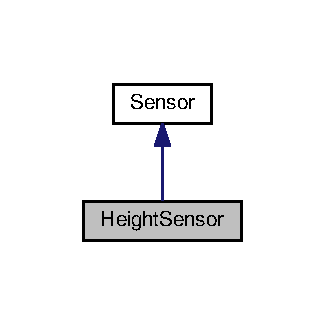
\includegraphics[width=156pt]{classHeightSensor__inherit__graph}
\end{center}
\end{figure}


Collaboration diagram for Height\+Sensor\+:\nopagebreak
\begin{figure}[H]
\begin{center}
\leavevmode
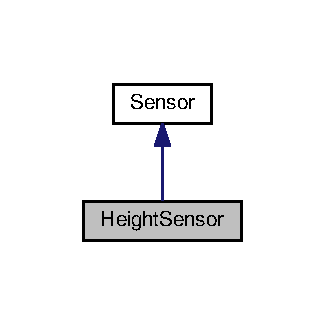
\includegraphics[width=156pt]{classHeightSensor__coll__graph}
\end{center}
\end{figure}
\subsection*{Public Member Functions}
\begin{DoxyCompactItemize}
\item 
{\bfseries Height\+Sensor} (int sensor\+Handle)\hypertarget{classHeightSensor_adce900c49d253c6e9cd85db00c2f0708}{}\label{classHeightSensor_adce900c49d253c6e9cd85db00c2f0708}

\item 
int \hyperlink{classHeightSensor_abd4b7d4cc5906a971da402757989f5da}{get} (std\+::vector$<$ float $>$ \&detect\+Point, int \&detect\+Handle, std\+::vector$<$ float $>$ \&detect\+Surface)
\item 
int \hyperlink{classHeightSensor_a90a19e600e5b89a503366da0f0c35590}{get} (std\+::vector$<$ float $>$ \&detect\+Point)
\item 
void \hyperlink{classHeightSensor_a6966090886a414a6213125c91a31e128}{update} (std\+::vector$<$ float $>$ \&f, int \&i, std\+::vector$<$ float $>$ \&ff)
\end{DoxyCompactItemize}
\subsection*{Additional Inherited Members}


\subsection{Detailed Description}
Implementation of a proximitysensor as height sensor. 

Class implementing a heightsensor 

\subsection{Member Function Documentation}
\index{Height\+Sensor@{Height\+Sensor}!get@{get}}
\index{get@{get}!Height\+Sensor@{Height\+Sensor}}
\subsubsection[{\texorpdfstring{get(std\+::vector$<$ float $>$ \&detect\+Point, int \&detect\+Handle, std\+::vector$<$ float $>$ \&detect\+Surface)}{get(std::vector< float > &detectPoint, int &detectHandle, std::vector< float > &detectSurface)}}]{\setlength{\rightskip}{0pt plus 5cm}int Height\+Sensor\+::get (
\begin{DoxyParamCaption}
\item[{std\+::vector$<$ float $>$ \&}]{detect\+Point, }
\item[{int \&}]{detect\+Handle, }
\item[{std\+::vector$<$ float $>$ \&}]{detect\+Surface}
\end{DoxyParamCaption}
)\hspace{0.3cm}{\ttfamily [virtual]}}\hypertarget{classHeightSensor_abd4b7d4cc5906a971da402757989f5da}{}\label{classHeightSensor_abd4b7d4cc5906a971da402757989f5da}
simply reads the sensor information with no additional call to handle the sensor in vrep 
\begin{DoxyParams}{Parameters}
{\em \&detect\+Point} & vector reference to store the coordinates of the closest point \\
\hline
{\em \&detect\+Handle} & integer reference to store the handle of the found object \\
\hline
{\em \&detect\+Surface} & vector reference to store the normal vector of the detected surface \\
\hline
\end{DoxyParams}


Implements \hyperlink{classSensor_a997a8679d48c4fa346e6ac43c1e6219a}{Sensor}.

\index{Height\+Sensor@{Height\+Sensor}!get@{get}}
\index{get@{get}!Height\+Sensor@{Height\+Sensor}}
\subsubsection[{\texorpdfstring{get(std\+::vector$<$ float $>$ \&detect\+Point)}{get(std::vector< float > &detectPoint)}}]{\setlength{\rightskip}{0pt plus 5cm}int Height\+Sensor\+::get (
\begin{DoxyParamCaption}
\item[{std\+::vector$<$ float $>$ \&}]{detect\+Point}
\end{DoxyParamCaption}
)\hspace{0.3cm}{\ttfamily [virtual]}}\hypertarget{classHeightSensor_a90a19e600e5b89a503366da0f0c35590}{}\label{classHeightSensor_a90a19e600e5b89a503366da0f0c35590}
same as the previous get, but all parameters except the coordinates of a detected point are omitted 

Implements \hyperlink{classSensor_a24f11619b11d5effc4066546629179ae}{Sensor}.

\index{Height\+Sensor@{Height\+Sensor}!update@{update}}
\index{update@{update}!Height\+Sensor@{Height\+Sensor}}
\subsubsection[{\texorpdfstring{update(std\+::vector$<$ float $>$ \&f, int \&i, std\+::vector$<$ float $>$ \&ff)}{update(std::vector< float > &f, int &i, std::vector< float > &ff)}}]{\setlength{\rightskip}{0pt plus 5cm}void Height\+Sensor\+::update (
\begin{DoxyParamCaption}
\item[{std\+::vector$<$ float $>$ \&}]{detect\+Point, }
\item[{int \&}]{detect\+Handle, }
\item[{std\+::vector$<$ float $>$ \&}]{detect\+Surface}
\end{DoxyParamCaption}
)\hspace{0.3cm}{\ttfamily [virtual]}}\hypertarget{classHeightSensor_a6966090886a414a6213125c91a31e128}{}\label{classHeightSensor_a6966090886a414a6213125c91a31e128}
calls for vrep to update the sensor information 
\begin{DoxyParams}{Parameters}
{\em \&detect\+Point} & vector reference to store the coordinates of the closest point \\
\hline
{\em \&detect\+Handle} & integer reference to store the handle of the found object \\
\hline
{\em \&detect\+Surface} & vector reference to store the normal vector of the detected surface \\
\hline
\end{DoxyParams}


Implements \hyperlink{classSensor_abb6c93c88529bc392d129443b3d352f3}{Sensor}.



The documentation for this class was generated from the following files\+:\begin{DoxyCompactItemize}
\item 
heightsensor.\+h\item 
\hyperlink{heightsensor_8cpp}{heightsensor.\+cpp}\end{DoxyCompactItemize}

\hypertarget{classLog}{}\section{Log Class Reference}
\label{classLog}\index{Log@{Log}}


Baisc logging class.  




{\ttfamily \#include $<$log.\+h$>$}



Collaboration diagram for Log\+:\nopagebreak
\begin{figure}[H]
\begin{center}
\leavevmode
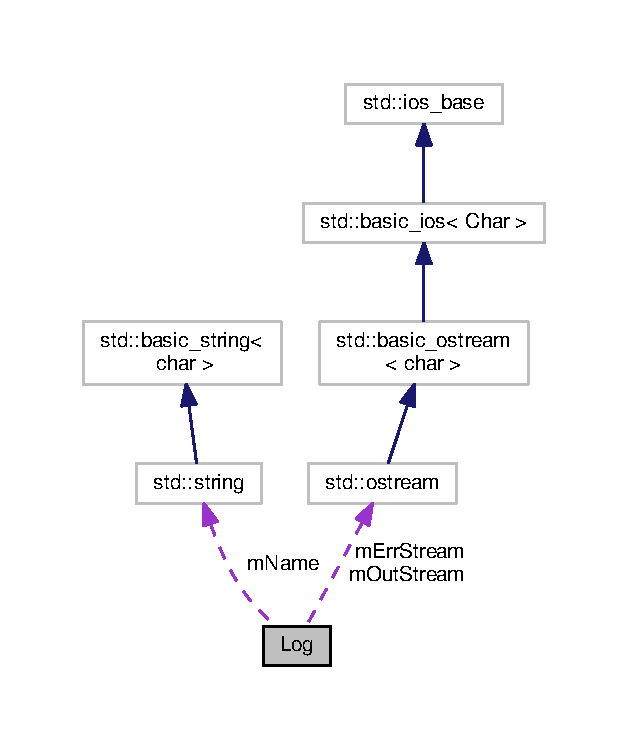
\includegraphics[width=302pt]{classLog__coll__graph}
\end{center}
\end{figure}
\subsection*{Public Member Functions}
\begin{DoxyCompactItemize}
\item 
\hyperlink{classLog_ac1cfcca90128605a5beec14beca019a2}{Log} ()=delete
\end{DoxyCompactItemize}
\subsection*{Static Public Member Functions}
\begin{DoxyCompactItemize}
\item 
static const std\+::ostream \& \hyperlink{classLog_a27b116b095e6e08d5e40fd365210c657}{out\+Stream} ()
\item 
static void \hyperlink{classLog_ad5a9c8a9d7f84d36041f21058f450e53}{out\+Stream} (std\+::ostream \&stream)
\item 
static const std\+::ostream \& \hyperlink{classLog_ac209747fd4964bc121818481ee131d19}{err\+Stream} ()
\item 
static void \hyperlink{classLog_ab2c566571ace5d3f234707ddfaaed4c9}{err\+Stream} (std\+::ostream \&stream)
\item 
static const std\+::string \& \hyperlink{classLog_a5a4518f9758b1eee0adcac1c3119288b}{name} ()
\item 
static void \hyperlink{classLog_a5758fde0052d1b682c6e2a33be192ecd}{name} (const std\+::string \&name)
\begin{DoxyCompactList}\small\item\em Sets the name to be shown in log messages. \end{DoxyCompactList}\item 
static std\+::ostream \& \hyperlink{classLog_ab89f6644dd040b1fa07c1253cc12bafb}{out} ()
\item 
static std\+::ostream \& \hyperlink{classLog_ad37da894b6f997bc5204ed81cace26c2}{err} ()
\end{DoxyCompactItemize}
\subsection*{Static Private Attributes}
\begin{DoxyCompactItemize}
\item 
static std\+::ostream $\ast$ \hyperlink{classLog_accbb35e5dcd2989a5a2085fc455e4685}{m\+Out\+Stream} =\&cout
\item 
static std\+::ostream $\ast$ \hyperlink{classLog_aa8469d1a7367bb976e1bc39514960ed5}{m\+Err\+Stream} =\&cerr
\item 
static std\+::string \hyperlink{classLog_a3c7121dc792ba672538009dd64585146}{m\+Name} =\char`\"{}Unknown\char`\"{}
\end{DoxyCompactItemize}


\subsection{Detailed Description}
Baisc logging class. 

\subsection{Constructor \& Destructor Documentation}
\index{Log@{Log}!Log@{Log}}
\index{Log@{Log}!Log@{Log}}
\subsubsection[{\texorpdfstring{Log()=delete}{Log()=delete}}]{\setlength{\rightskip}{0pt plus 5cm}Log\+::\+Log (
\begin{DoxyParamCaption}
{}
\end{DoxyParamCaption}
)\hspace{0.3cm}{\ttfamily [delete]}}\hypertarget{classLog_ac1cfcca90128605a5beec14beca019a2}{}\label{classLog_ac1cfcca90128605a5beec14beca019a2}


\subsection{Member Function Documentation}
\index{Log@{Log}!err@{err}}
\index{err@{err}!Log@{Log}}
\subsubsection[{\texorpdfstring{err()}{err()}}]{\setlength{\rightskip}{0pt plus 5cm}static std\+::ostream\& Log\+::err (
\begin{DoxyParamCaption}
{}
\end{DoxyParamCaption}
)\hspace{0.3cm}{\ttfamily [inline]}, {\ttfamily [static]}}\hypertarget{classLog_ad37da894b6f997bc5204ed81cace26c2}{}\label{classLog_ad37da894b6f997bc5204ed81cace26c2}


Here is the call graph for this function\+:\nopagebreak
\begin{figure}[H]
\begin{center}
\leavevmode
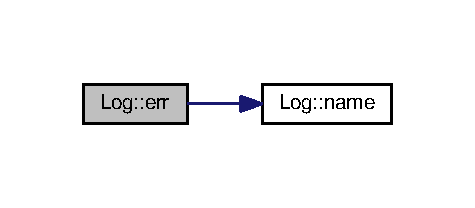
\includegraphics[width=228pt]{classLog_ad37da894b6f997bc5204ed81cace26c2_cgraph}
\end{center}
\end{figure}


\index{Log@{Log}!err\+Stream@{err\+Stream}}
\index{err\+Stream@{err\+Stream}!Log@{Log}}
\subsubsection[{\texorpdfstring{err\+Stream()}{errStream()}}]{\setlength{\rightskip}{0pt plus 5cm}static const std\+::ostream\& Log\+::err\+Stream (
\begin{DoxyParamCaption}
{}
\end{DoxyParamCaption}
)\hspace{0.3cm}{\ttfamily [inline]}, {\ttfamily [static]}}\hypertarget{classLog_ac209747fd4964bc121818481ee131d19}{}\label{classLog_ac209747fd4964bc121818481ee131d19}
\index{Log@{Log}!err\+Stream@{err\+Stream}}
\index{err\+Stream@{err\+Stream}!Log@{Log}}
\subsubsection[{\texorpdfstring{err\+Stream(std\+::ostream \&stream)}{errStream(std::ostream &stream)}}]{\setlength{\rightskip}{0pt plus 5cm}static void Log\+::err\+Stream (
\begin{DoxyParamCaption}
\item[{std\+::ostream \&}]{stream}
\end{DoxyParamCaption}
)\hspace{0.3cm}{\ttfamily [inline]}, {\ttfamily [static]}}\hypertarget{classLog_ab2c566571ace5d3f234707ddfaaed4c9}{}\label{classLog_ab2c566571ace5d3f234707ddfaaed4c9}
\index{Log@{Log}!name@{name}}
\index{name@{name}!Log@{Log}}
\subsubsection[{\texorpdfstring{name()}{name()}}]{\setlength{\rightskip}{0pt plus 5cm}static const std\+::string\& Log\+::name (
\begin{DoxyParamCaption}
{}
\end{DoxyParamCaption}
)\hspace{0.3cm}{\ttfamily [inline]}, {\ttfamily [static]}}\hypertarget{classLog_a5a4518f9758b1eee0adcac1c3119288b}{}\label{classLog_a5a4518f9758b1eee0adcac1c3119288b}


Here is the caller graph for this function\+:\nopagebreak
\begin{figure}[H]
\begin{center}
\leavevmode
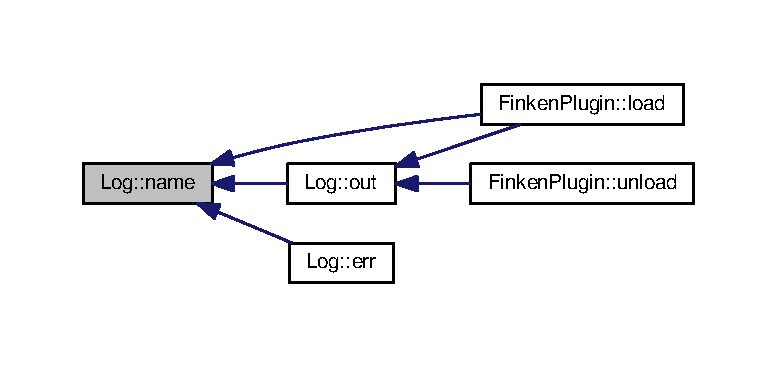
\includegraphics[width=350pt]{classLog_a5a4518f9758b1eee0adcac1c3119288b_icgraph}
\end{center}
\end{figure}


\index{Log@{Log}!name@{name}}
\index{name@{name}!Log@{Log}}
\subsubsection[{\texorpdfstring{name(const std\+::string \&name)}{name(const std::string &name)}}]{\setlength{\rightskip}{0pt plus 5cm}static void Log\+::name (
\begin{DoxyParamCaption}
\item[{const std\+::string \&}]{name}
\end{DoxyParamCaption}
)\hspace{0.3cm}{\ttfamily [inline]}, {\ttfamily [static]}}\hypertarget{classLog_a5758fde0052d1b682c6e2a33be192ecd}{}\label{classLog_a5758fde0052d1b682c6e2a33be192ecd}


Sets the name to be shown in log messages. 



Here is the call graph for this function\+:\nopagebreak
\begin{figure}[H]
\begin{center}
\leavevmode
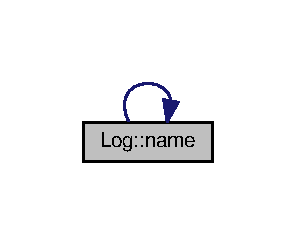
\includegraphics[width=142pt]{classLog_a5758fde0052d1b682c6e2a33be192ecd_cgraph}
\end{center}
\end{figure}




Here is the caller graph for this function\+:\nopagebreak
\begin{figure}[H]
\begin{center}
\leavevmode
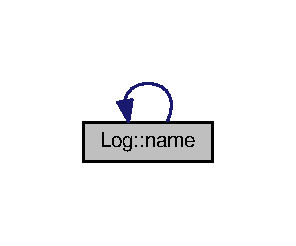
\includegraphics[width=142pt]{classLog_a5758fde0052d1b682c6e2a33be192ecd_icgraph}
\end{center}
\end{figure}


\index{Log@{Log}!out@{out}}
\index{out@{out}!Log@{Log}}
\subsubsection[{\texorpdfstring{out()}{out()}}]{\setlength{\rightskip}{0pt plus 5cm}static std\+::ostream\& Log\+::out (
\begin{DoxyParamCaption}
{}
\end{DoxyParamCaption}
)\hspace{0.3cm}{\ttfamily [inline]}, {\ttfamily [static]}}\hypertarget{classLog_ab89f6644dd040b1fa07c1253cc12bafb}{}\label{classLog_ab89f6644dd040b1fa07c1253cc12bafb}


Here is the call graph for this function\+:\nopagebreak
\begin{figure}[H]
\begin{center}
\leavevmode
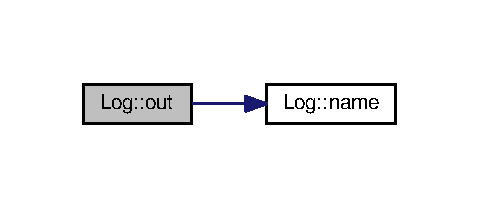
\includegraphics[width=230pt]{classLog_ab89f6644dd040b1fa07c1253cc12bafb_cgraph}
\end{center}
\end{figure}




Here is the caller graph for this function\+:\nopagebreak
\begin{figure}[H]
\begin{center}
\leavevmode
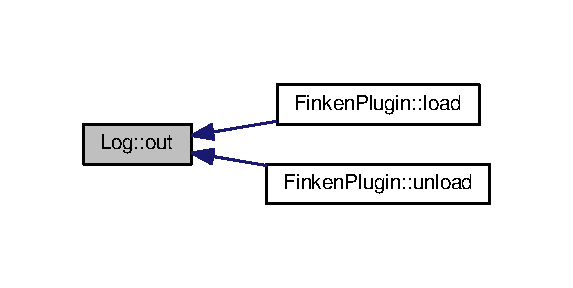
\includegraphics[width=275pt]{classLog_ab89f6644dd040b1fa07c1253cc12bafb_icgraph}
\end{center}
\end{figure}


\index{Log@{Log}!out\+Stream@{out\+Stream}}
\index{out\+Stream@{out\+Stream}!Log@{Log}}
\subsubsection[{\texorpdfstring{out\+Stream()}{outStream()}}]{\setlength{\rightskip}{0pt plus 5cm}static const std\+::ostream\& Log\+::out\+Stream (
\begin{DoxyParamCaption}
{}
\end{DoxyParamCaption}
)\hspace{0.3cm}{\ttfamily [inline]}, {\ttfamily [static]}}\hypertarget{classLog_a27b116b095e6e08d5e40fd365210c657}{}\label{classLog_a27b116b095e6e08d5e40fd365210c657}
\index{Log@{Log}!out\+Stream@{out\+Stream}}
\index{out\+Stream@{out\+Stream}!Log@{Log}}
\subsubsection[{\texorpdfstring{out\+Stream(std\+::ostream \&stream)}{outStream(std::ostream &stream)}}]{\setlength{\rightskip}{0pt plus 5cm}static void Log\+::out\+Stream (
\begin{DoxyParamCaption}
\item[{std\+::ostream \&}]{stream}
\end{DoxyParamCaption}
)\hspace{0.3cm}{\ttfamily [inline]}, {\ttfamily [static]}}\hypertarget{classLog_ad5a9c8a9d7f84d36041f21058f450e53}{}\label{classLog_ad5a9c8a9d7f84d36041f21058f450e53}


\subsection{Member Data Documentation}
\index{Log@{Log}!m\+Err\+Stream@{m\+Err\+Stream}}
\index{m\+Err\+Stream@{m\+Err\+Stream}!Log@{Log}}
\subsubsection[{\texorpdfstring{m\+Err\+Stream}{mErrStream}}]{\setlength{\rightskip}{0pt plus 5cm}ostream $\ast$ Log\+::m\+Err\+Stream =\&cerr\hspace{0.3cm}{\ttfamily [static]}, {\ttfamily [private]}}\hypertarget{classLog_aa8469d1a7367bb976e1bc39514960ed5}{}\label{classLog_aa8469d1a7367bb976e1bc39514960ed5}
\index{Log@{Log}!m\+Name@{m\+Name}}
\index{m\+Name@{m\+Name}!Log@{Log}}
\subsubsection[{\texorpdfstring{m\+Name}{mName}}]{\setlength{\rightskip}{0pt plus 5cm}string Log\+::m\+Name =\char`\"{}Unknown\char`\"{}\hspace{0.3cm}{\ttfamily [static]}, {\ttfamily [private]}}\hypertarget{classLog_a3c7121dc792ba672538009dd64585146}{}\label{classLog_a3c7121dc792ba672538009dd64585146}
\index{Log@{Log}!m\+Out\+Stream@{m\+Out\+Stream}}
\index{m\+Out\+Stream@{m\+Out\+Stream}!Log@{Log}}
\subsubsection[{\texorpdfstring{m\+Out\+Stream}{mOutStream}}]{\setlength{\rightskip}{0pt plus 5cm}ostream $\ast$ Log\+::m\+Out\+Stream =\&cout\hspace{0.3cm}{\ttfamily [static]}, {\ttfamily [private]}}\hypertarget{classLog_accbb35e5dcd2989a5a2085fc455e4685}{}\label{classLog_accbb35e5dcd2989a5a2085fc455e4685}


The documentation for this class was generated from the following files\+:\begin{DoxyCompactItemize}
\item 
\hyperlink{log_8h}{log.\+h}\item 
\hyperlink{log_8cpp}{log.\+cpp}\end{DoxyCompactItemize}

\hypertarget{classLogLine}{}\section{Log\+Line Class Reference}
\label{classLogLine}\index{Log\+Line@{Log\+Line}}


Class for annotating log with time points.  




{\ttfamily \#include $<$finken.\+h$>$}

\subsection*{Public Member Functions}
\begin{DoxyCompactItemize}
\item 
{\bfseries Log\+Line} (std\+::ostream \&o)\hypertarget{classLogLine_a7f1c876fef642fffb06f646749662a04}{}\label{classLogLine_a7f1c876fef642fffb06f646749662a04}

\item 
\hyperlink{classLogLine}{Log\+Line} \& {\bfseries operator$<$$<$} (std\+::ostream \&($\ast$pf)(std\+::ostream \&))\hypertarget{classLogLine_a9697d8126ee9dd2ee3ea70bc61abf4b8}{}\label{classLogLine_a9697d8126ee9dd2ee3ea70bc61abf4b8}

\item 
{\footnotesize template$<$typename T $>$ }\\\hyperlink{classLogLine}{Log\+Line} \& {\bfseries operator$<$$<$} (T t)\hypertarget{classLogLine_aa9dff12f0c1466e53e63f981872f1e76}{}\label{classLogLine_aa9dff12f0c1466e53e63f981872f1e76}

\end{DoxyCompactItemize}
\subsection*{Friends}
\begin{DoxyCompactItemize}
\item 
class {\bfseries Vrep\+Log}\hypertarget{classLogLine_a4b85b5c9be56c4b49e99130f36f2df1d}{}\label{classLogLine_a4b85b5c9be56c4b49e99130f36f2df1d}

\end{DoxyCompactItemize}


\subsection{Detailed Description}
Class for annotating log with time points. 

\begin{DoxyRefDesc}{Todo}
\item[\hyperlink{todo__todo000003}{Todo}]cleanup code from superfluous debug logging \end{DoxyRefDesc}


The documentation for this class was generated from the following file\+:\begin{DoxyCompactItemize}
\item 
\hyperlink{finken_8h}{finken.\+h}\end{DoxyCompactItemize}

\hypertarget{classPositionSensor}{}\section{Position\+Sensor Class Reference}
\label{classPositionSensor}\index{Position\+Sensor@{Position\+Sensor}}


wrapper to disguise vrep A\+PI calls as a position sensor  




Inheritance diagram for Position\+Sensor\+:\nopagebreak
\begin{figure}[H]
\begin{center}
\leavevmode
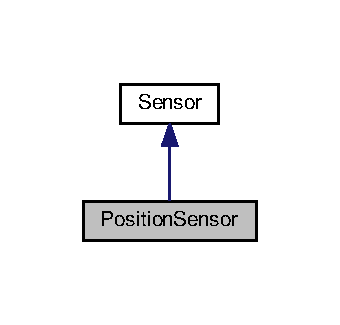
\includegraphics[width=163pt]{classPositionSensor__inherit__graph}
\end{center}
\end{figure}


Collaboration diagram for Position\+Sensor\+:\nopagebreak
\begin{figure}[H]
\begin{center}
\leavevmode
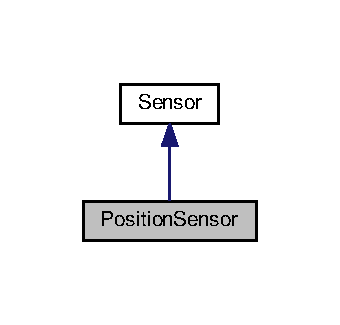
\includegraphics[width=163pt]{classPositionSensor__coll__graph}
\end{center}
\end{figure}
\subsection*{Public Member Functions}
\begin{DoxyCompactItemize}
\item 
{\bfseries Position\+Sensor} (int sensor\+Handle)\hypertarget{classPositionSensor_a1bc5cb93c92c04eef26d406dbb304ead}{}\label{classPositionSensor_a1bc5cb93c92c04eef26d406dbb304ead}

\item 
int \hyperlink{classPositionSensor_a99c4b37f9f16912b15603d79dda386bc}{get} (std\+::vector$<$ float $>$ \&detect\+Position)
\item 
void \hyperlink{classPositionSensor_a4fb083aa0462a73627b11b7c0e408f09}{update} (std\+::vector$<$ float $>$ \&f, int \&i, std\+::vector$<$ float $>$ \&ff)
\item 
int \hyperlink{classPositionSensor_a0b8c45d846d3442d94e2ef767fddf31d}{get} (std\+::vector$<$ float $>$ \&detect\+Point, int \&detect\+Handle, std\+::vector$<$ float $>$ \&detect\+Surface)
\end{DoxyCompactItemize}
\subsection*{Additional Inherited Members}


\subsection{Detailed Description}
wrapper to disguise vrep A\+PI calls as a position sensor 

\begin{DoxyRefDesc}{Todo}
\item[\hyperlink{todo__todo000006}{Todo}]actually use this in the sim \end{DoxyRefDesc}


\subsection{Member Function Documentation}
\index{Position\+Sensor@{Position\+Sensor}!get@{get}}
\index{get@{get}!Position\+Sensor@{Position\+Sensor}}
\subsubsection[{\texorpdfstring{get(std\+::vector$<$ float $>$ \&detect\+Position)}{get(std::vector< float > &detectPosition)}}]{\setlength{\rightskip}{0pt plus 5cm}int Position\+Sensor\+::get (
\begin{DoxyParamCaption}
\item[{std\+::vector$<$ float $>$ \&}]{vfloat}
\end{DoxyParamCaption}
)\hspace{0.3cm}{\ttfamily [virtual]}}\hypertarget{classPositionSensor_a99c4b37f9f16912b15603d79dda386bc}{}\label{classPositionSensor_a99c4b37f9f16912b15603d79dda386bc}
retrieves the sensor information, limited to the position of a detected object; see specific sensor documentation for parameter information 

Implements \hyperlink{classSensor_a24f11619b11d5effc4066546629179ae}{Sensor}.

\index{Position\+Sensor@{Position\+Sensor}!get@{get}}
\index{get@{get}!Position\+Sensor@{Position\+Sensor}}
\subsubsection[{\texorpdfstring{get(std\+::vector$<$ float $>$ \&detect\+Point, int \&detect\+Handle, std\+::vector$<$ float $>$ \&detect\+Surface)}{get(std::vector< float > &detectPoint, int &detectHandle, std::vector< float > &detectSurface)}}]{\setlength{\rightskip}{0pt plus 5cm}int Position\+Sensor\+::get (
\begin{DoxyParamCaption}
\item[{std\+::vector$<$ float $>$ \&}]{detect\+Point, }
\item[{int \&}]{detect\+Handle, }
\item[{std\+::vector$<$ float $>$ \&}]{detect\+Surface}
\end{DoxyParamCaption}
)\hspace{0.3cm}{\ttfamily [virtual]}}\hypertarget{classPositionSensor_a0b8c45d846d3442d94e2ef767fddf31d}{}\label{classPositionSensor_a0b8c45d846d3442d94e2ef767fddf31d}
retrieves the sensor information, including any detected object information; see specific sensor documentation for paramter information 

Implements \hyperlink{classSensor_a997a8679d48c4fa346e6ac43c1e6219a}{Sensor}.

\index{Position\+Sensor@{Position\+Sensor}!update@{update}}
\index{update@{update}!Position\+Sensor@{Position\+Sensor}}
\subsubsection[{\texorpdfstring{update(std\+::vector$<$ float $>$ \&f, int \&i, std\+::vector$<$ float $>$ \&ff)}{update(std::vector< float > &f, int &i, std::vector< float > &ff)}}]{\setlength{\rightskip}{0pt plus 5cm}void Position\+Sensor\+::update (
\begin{DoxyParamCaption}
\item[{std\+::vector$<$ float $>$ \&}]{f, }
\item[{int \&}]{i, }
\item[{std\+::vector$<$ float $>$ \&}]{ff}
\end{DoxyParamCaption}
)\hspace{0.3cm}{\ttfamily [virtual]}}\hypertarget{classPositionSensor_a4fb083aa0462a73627b11b7c0e408f09}{}\label{classPositionSensor_a4fb083aa0462a73627b11b7c0e408f09}
calls for Vrep to update the sensor information; see specific sensor documentation for parameter information 

Implements \hyperlink{classSensor_abb6c93c88529bc392d129443b3d352f3}{Sensor}.



The documentation for this class was generated from the following files\+:\begin{DoxyCompactItemize}
\item 
positionsensor.\+h\item 
\hyperlink{positionsensor_8cpp}{positionsensor.\+cpp}\end{DoxyCompactItemize}

\hypertarget{classRotor}{}\section{Rotor Class Reference}
\label{classRotor}\index{Rotor@{Rotor}}


Implementation of a force sensor as a rotor.  




{\ttfamily \#include $<$rotor.\+h$>$}

\subsection*{Public Member Functions}
\begin{DoxyCompactItemize}
\item 
\hyperlink{classRotor_ab1ad46cf401db508602fb136f09094c2}{Rotor} (int r\+Handle)
\begin{DoxyCompactList}\small\item\em Basic constructor. \end{DoxyCompactList}\item 
void \hyperlink{classRotor_aa961955180593d6249b3c35730b29cfb}{set} (const std\+::vector$<$ float $>$ \&force, const std\+::vector$<$ float $>$ \&torque)
\begin{DoxyCompactList}\small\item\em Function to set the force and torque fvalues or the rotor. \end{DoxyCompactList}\end{DoxyCompactItemize}
\subsection*{Public Attributes}
\begin{DoxyCompactItemize}
\item 
int \hyperlink{classRotor_ae6da9102b10f4759201a62117f6b2b6e}{handle}
\begin{DoxyCompactList}\small\item\em Handle to access the sensor in V-\/\+R\+EP. \end{DoxyCompactList}\end{DoxyCompactItemize}


\subsection{Detailed Description}
Implementation of a force sensor as a rotor. 

\subsection{Constructor \& Destructor Documentation}
\index{Rotor@{Rotor}!Rotor@{Rotor}}
\index{Rotor@{Rotor}!Rotor@{Rotor}}
\subsubsection[{\texorpdfstring{Rotor(int r\+Handle)}{Rotor(int rHandle)}}]{\setlength{\rightskip}{0pt plus 5cm}Rotor\+::\+Rotor (
\begin{DoxyParamCaption}
\item[{int}]{r\+Handle}
\end{DoxyParamCaption}
)}\hypertarget{classRotor_ab1ad46cf401db508602fb136f09094c2}{}\label{classRotor_ab1ad46cf401db508602fb136f09094c2}


Basic constructor. 


\begin{DoxyParams}{Parameters}
{\em r\+Handle} & the handle of the sensor in V-\/\+R\+EP \\
\hline
\end{DoxyParams}


\subsection{Member Function Documentation}
\index{Rotor@{Rotor}!set@{set}}
\index{set@{set}!Rotor@{Rotor}}
\subsubsection[{\texorpdfstring{set(const std\+::vector$<$ float $>$ \&force, const std\+::vector$<$ float $>$ \&torque)}{set(const std::vector< float > &force, const std::vector< float > &torque)}}]{\setlength{\rightskip}{0pt plus 5cm}void Rotor\+::set (
\begin{DoxyParamCaption}
\item[{const std\+::vector$<$ float $>$ \&}]{force, }
\item[{const std\+::vector$<$ float $>$ \&}]{torque}
\end{DoxyParamCaption}
)}\hypertarget{classRotor_aa961955180593d6249b3c35730b29cfb}{}\label{classRotor_aa961955180593d6249b3c35730b29cfb}


Function to set the force and torque fvalues or the rotor. 


\begin{DoxyParams}{Parameters}
{\em force} & The force to be applied. \\
\hline
{\em torque} & The torque to be applied.\\
\hline
\end{DoxyParams}
See the \href{http://www.coppeliarobotics.com/helpFiles/en/regularApi/simAddForceAndTorque.htm}{\tt V-\/\+R\+EP A\+PI} for more info. 

\subsection{Member Data Documentation}
\index{Rotor@{Rotor}!handle@{handle}}
\index{handle@{handle}!Rotor@{Rotor}}
\subsubsection[{\texorpdfstring{handle}{handle}}]{\setlength{\rightskip}{0pt plus 5cm}int Rotor\+::handle}\hypertarget{classRotor_ae6da9102b10f4759201a62117f6b2b6e}{}\label{classRotor_ae6da9102b10f4759201a62117f6b2b6e}


Handle to access the sensor in V-\/\+R\+EP. 



The documentation for this class was generated from the following files\+:\begin{DoxyCompactItemize}
\item 
\hyperlink{rotor_8h}{rotor.\+h}\item 
\hyperlink{rotor_8cpp}{rotor.\+cpp}\end{DoxyCompactItemize}

\hypertarget{classSensor}{}\section{Sensor Class Reference}
\label{classSensor}\index{Sensor@{Sensor}}


base \hyperlink{classSensor}{Sensor} class, all sensors should inherit from this  




{\ttfamily \#include $<$sensor.\+h$>$}



Inheritance diagram for Sensor\+:\nopagebreak
\begin{figure}[H]
\begin{center}
\leavevmode
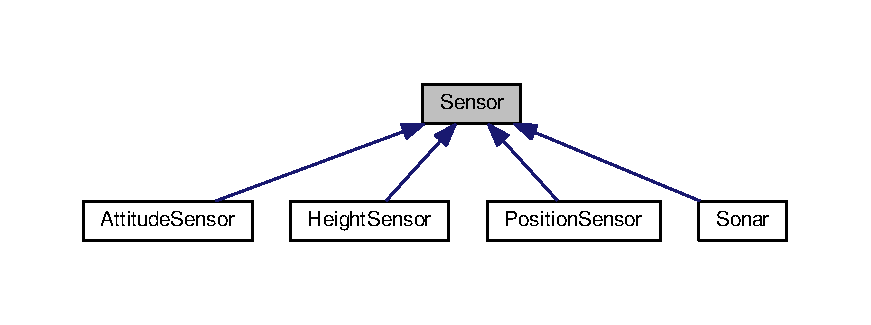
\includegraphics[width=350pt]{classSensor__inherit__graph}
\end{center}
\end{figure}
\subsection*{Public Member Functions}
\begin{DoxyCompactItemize}
\item 
\hyperlink{classSensor_aec15220e0b38da37e43b0525ac689499}{Sensor} (int sensor\+Handle)
\item 
virtual void \hyperlink{classSensor_abb6c93c88529bc392d129443b3d352f3}{update} (std\+::vector$<$ float $>$ \&f, int \&i, std\+::vector$<$ float $>$ \&ff)=0
\item 
virtual int \hyperlink{classSensor_a997a8679d48c4fa346e6ac43c1e6219a}{get} (std\+::vector$<$ float $>$ \&detect\+Point, int \&detect\+Handle, std\+::vector$<$ float $>$ \&detect\+Surface)=0
\item 
virtual int \hyperlink{classSensor_a24f11619b11d5effc4066546629179ae}{get} (std\+::vector$<$ float $>$ \&vfloat)=0
\item 
virtual int {\bfseries get\+Handle} ()\hypertarget{classSensor_ac647e98897da5ffcc9711ba27ec45abd}{}\label{classSensor_ac647e98897da5ffcc9711ba27ec45abd}

\end{DoxyCompactItemize}
\subsection*{Protected Attributes}
\begin{DoxyCompactItemize}
\item 
int \hyperlink{classSensor_ad31f2503e8a1cc7888e5eefbeede8f3b}{handle}
\end{DoxyCompactItemize}


\subsection{Detailed Description}
base \hyperlink{classSensor}{Sensor} class, all sensors should inherit from this 

Basic \hyperlink{classSensor}{Sensor} class from which specialized sensors are derived 

\subsection{Constructor \& Destructor Documentation}
\index{Sensor@{Sensor}!Sensor@{Sensor}}
\index{Sensor@{Sensor}!Sensor@{Sensor}}
\subsubsection[{\texorpdfstring{Sensor(int sensor\+Handle)}{Sensor(int sensorHandle)}}]{\setlength{\rightskip}{0pt plus 5cm}Sensor\+::\+Sensor (
\begin{DoxyParamCaption}
\item[{int}]{sensor\+Handle}
\end{DoxyParamCaption}
)}\hypertarget{classSensor_aec15220e0b38da37e43b0525ac689499}{}\label{classSensor_aec15220e0b38da37e43b0525ac689499}
Constructor 
\begin{DoxyParams}{Parameters}
{\em sensor\+Handle} & the handle of the sensor in vrep \\
\hline
\end{DoxyParams}


\subsection{Member Function Documentation}
\index{Sensor@{Sensor}!get@{get}}
\index{get@{get}!Sensor@{Sensor}}
\subsubsection[{\texorpdfstring{get(std\+::vector$<$ float $>$ \&detect\+Point, int \&detect\+Handle, std\+::vector$<$ float $>$ \&detect\+Surface)=0}{get(std::vector< float > &detectPoint, int &detectHandle, std::vector< float > &detectSurface)=0}}]{\setlength{\rightskip}{0pt plus 5cm}virtual int Sensor\+::get (
\begin{DoxyParamCaption}
\item[{std\+::vector$<$ float $>$ \&}]{detect\+Point, }
\item[{int \&}]{detect\+Handle, }
\item[{std\+::vector$<$ float $>$ \&}]{detect\+Surface}
\end{DoxyParamCaption}
)\hspace{0.3cm}{\ttfamily [pure virtual]}}\hypertarget{classSensor_a997a8679d48c4fa346e6ac43c1e6219a}{}\label{classSensor_a997a8679d48c4fa346e6ac43c1e6219a}
retrieves the sensor information, including any detected object information; see specific sensor documentation for paramter information 

Implemented in \hyperlink{classAttitudeSensor_a29d069767d7b3b36a998ae70764134dd}{Attitude\+Sensor}, \hyperlink{classHeightSensor_abd4b7d4cc5906a971da402757989f5da}{Height\+Sensor}, \hyperlink{classPositionSensor_a0b8c45d846d3442d94e2ef767fddf31d}{Position\+Sensor}, and \hyperlink{classSonar_a6881d0c104c0fafad95ad1aea917b6f3}{Sonar}.

\index{Sensor@{Sensor}!get@{get}}
\index{get@{get}!Sensor@{Sensor}}
\subsubsection[{\texorpdfstring{get(std\+::vector$<$ float $>$ \&vfloat)=0}{get(std::vector< float > &vfloat)=0}}]{\setlength{\rightskip}{0pt plus 5cm}virtual int Sensor\+::get (
\begin{DoxyParamCaption}
\item[{std\+::vector$<$ float $>$ \&}]{vfloat}
\end{DoxyParamCaption}
)\hspace{0.3cm}{\ttfamily [pure virtual]}}\hypertarget{classSensor_a24f11619b11d5effc4066546629179ae}{}\label{classSensor_a24f11619b11d5effc4066546629179ae}
retrieves the sensor information, limited to the position of a detected object; see specific sensor documentation for parameter information 

Implemented in \hyperlink{classAttitudeSensor_a354f56cfccea6f60b4822b9e2603afc8}{Attitude\+Sensor}, \hyperlink{classHeightSensor_a90a19e600e5b89a503366da0f0c35590}{Height\+Sensor}, \hyperlink{classPositionSensor_a99c4b37f9f16912b15603d79dda386bc}{Position\+Sensor}, and \hyperlink{classSonar_af77f9c5b9db42276b06b3b044c738284}{Sonar}.

\index{Sensor@{Sensor}!update@{update}}
\index{update@{update}!Sensor@{Sensor}}
\subsubsection[{\texorpdfstring{update(std\+::vector$<$ float $>$ \&f, int \&i, std\+::vector$<$ float $>$ \&ff)=0}{update(std::vector< float > &f, int &i, std::vector< float > &ff)=0}}]{\setlength{\rightskip}{0pt plus 5cm}virtual void Sensor\+::update (
\begin{DoxyParamCaption}
\item[{std\+::vector$<$ float $>$ \&}]{f, }
\item[{int \&}]{i, }
\item[{std\+::vector$<$ float $>$ \&}]{ff}
\end{DoxyParamCaption}
)\hspace{0.3cm}{\ttfamily [pure virtual]}}\hypertarget{classSensor_abb6c93c88529bc392d129443b3d352f3}{}\label{classSensor_abb6c93c88529bc392d129443b3d352f3}
calls for Vrep to update the sensor information; see specific sensor documentation for parameter information 

Implemented in \hyperlink{classAttitudeSensor_a035c43c2ae16df0dedbbc7ae4cb575d9}{Attitude\+Sensor}, \hyperlink{classHeightSensor_a6966090886a414a6213125c91a31e128}{Height\+Sensor}, \hyperlink{classPositionSensor_a4fb083aa0462a73627b11b7c0e408f09}{Position\+Sensor}, and \hyperlink{classSonar_ab32f714b0c5412e64ec60997467074bc}{Sonar}.



\subsection{Member Data Documentation}
\index{Sensor@{Sensor}!handle@{handle}}
\index{handle@{handle}!Sensor@{Sensor}}
\subsubsection[{\texorpdfstring{handle}{handle}}]{\setlength{\rightskip}{0pt plus 5cm}int Sensor\+::handle\hspace{0.3cm}{\ttfamily [protected]}}\hypertarget{classSensor_ad31f2503e8a1cc7888e5eefbeede8f3b}{}\label{classSensor_ad31f2503e8a1cc7888e5eefbeede8f3b}
Handle to access the sensor in vrep 

The documentation for this class was generated from the following files\+:\begin{DoxyCompactItemize}
\item 
sensor.\+h\item 
\hyperlink{sensor_8cpp}{sensor.\+cpp}\end{DoxyCompactItemize}

\hypertarget{classSonar}{}\section{Sonar Class Reference}
\label{classSonar}\index{Sonar@{Sonar}}


implementation of a proximitysensor as sonar  




Inheritance diagram for Sonar\+:\nopagebreak
\begin{figure}[H]
\begin{center}
\leavevmode
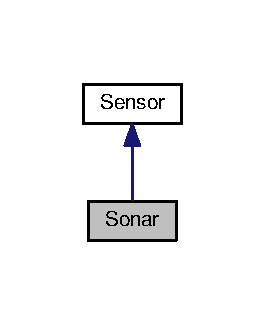
\includegraphics[width=127pt]{classSonar__inherit__graph}
\end{center}
\end{figure}


Collaboration diagram for Sonar\+:\nopagebreak
\begin{figure}[H]
\begin{center}
\leavevmode
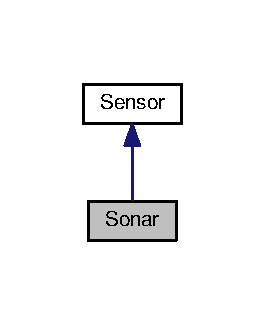
\includegraphics[width=127pt]{classSonar__coll__graph}
\end{center}
\end{figure}
\subsection*{Public Member Functions}
\begin{DoxyCompactItemize}
\item 
{\bfseries Sonar} (int sensor\+Handle)\hypertarget{classSonar_ae6edd4f329f9892a64c5f0cab808c7a2}{}\label{classSonar_ae6edd4f329f9892a64c5f0cab808c7a2}

\item 
int \hyperlink{classSonar_a6881d0c104c0fafad95ad1aea917b6f3}{get} (std\+::vector$<$ float $>$ \&detect\+Point, int \&detect\+Handle, std\+::vector$<$ float $>$ \&detect\+Surface)
\item 
int \hyperlink{classSonar_af77f9c5b9db42276b06b3b044c738284}{get} (std\+::vector$<$ float $>$ \&detect\+Point)
\item 
void \hyperlink{classSonar_ab32f714b0c5412e64ec60997467074bc}{update} (std\+::vector$<$ float $>$ \&f, int \&i, std\+::vector$<$ float $>$ \&ff)
\end{DoxyCompactItemize}
\subsection*{Additional Inherited Members}


\subsection{Detailed Description}
implementation of a proximitysensor as sonar 

\begin{DoxyRefDesc}{Todo}
\item[\hyperlink{todo__todo000007}{Todo}]actually use this in the sim \end{DoxyRefDesc}


\subsection{Member Function Documentation}
\index{Sonar@{Sonar}!get@{get}}
\index{get@{get}!Sonar@{Sonar}}
\subsubsection[{\texorpdfstring{get(std\+::vector$<$ float $>$ \&detect\+Point, int \&detect\+Handle, std\+::vector$<$ float $>$ \&detect\+Surface)}{get(std::vector< float > &detectPoint, int &detectHandle, std::vector< float > &detectSurface)}}]{\setlength{\rightskip}{0pt plus 5cm}int Sonar\+::get (
\begin{DoxyParamCaption}
\item[{std\+::vector$<$ float $>$ \&}]{detect\+Point, }
\item[{int \&}]{detect\+Handle, }
\item[{std\+::vector$<$ float $>$ \&}]{detect\+Surface}
\end{DoxyParamCaption}
)\hspace{0.3cm}{\ttfamily [virtual]}}\hypertarget{classSonar_a6881d0c104c0fafad95ad1aea917b6f3}{}\label{classSonar_a6881d0c104c0fafad95ad1aea917b6f3}
simply reads the sensor information with no additional call to handle the sensor in vrep 
\begin{DoxyParams}{Parameters}
{\em \&detect\+Point} & vector reference to store the coordinates of the closest point \\
\hline
{\em \&detect\+Handle} & integer reference to store the handle of the found object \\
\hline
{\em \&detect\+Surface} & vector reference to store the normal vector of the detected surface \\
\hline
\end{DoxyParams}


Implements \hyperlink{classSensor_a997a8679d48c4fa346e6ac43c1e6219a}{Sensor}.

\index{Sonar@{Sonar}!get@{get}}
\index{get@{get}!Sonar@{Sonar}}
\subsubsection[{\texorpdfstring{get(std\+::vector$<$ float $>$ \&detect\+Point)}{get(std::vector< float > &detectPoint)}}]{\setlength{\rightskip}{0pt plus 5cm}int Sonar\+::get (
\begin{DoxyParamCaption}
\item[{std\+::vector$<$ float $>$ \&}]{detect\+Point}
\end{DoxyParamCaption}
)\hspace{0.3cm}{\ttfamily [virtual]}}\hypertarget{classSonar_af77f9c5b9db42276b06b3b044c738284}{}\label{classSonar_af77f9c5b9db42276b06b3b044c738284}
same as the previous get, but all parameters except the coordinates of a detected point are omitted 

Implements \hyperlink{classSensor_a24f11619b11d5effc4066546629179ae}{Sensor}.

\index{Sonar@{Sonar}!update@{update}}
\index{update@{update}!Sonar@{Sonar}}
\subsubsection[{\texorpdfstring{update(std\+::vector$<$ float $>$ \&f, int \&i, std\+::vector$<$ float $>$ \&ff)}{update(std::vector< float > &f, int &i, std::vector< float > &ff)}}]{\setlength{\rightskip}{0pt plus 5cm}void Sonar\+::update (
\begin{DoxyParamCaption}
\item[{std\+::vector$<$ float $>$ \&}]{f, }
\item[{int \&}]{i, }
\item[{std\+::vector$<$ float $>$ \&}]{ff}
\end{DoxyParamCaption}
)\hspace{0.3cm}{\ttfamily [virtual]}}\hypertarget{classSonar_ab32f714b0c5412e64ec60997467074bc}{}\label{classSonar_ab32f714b0c5412e64ec60997467074bc}
calls for vrep to update the sensor information 
\begin{DoxyParams}{Parameters}
{\em \&detect\+Point} & vector reference to store the coordinates of the closest point \\
\hline
{\em \&detect\+Handle} & integer reference to store the handle of the found object \\
\hline
{\em \&detect\+Surface} & vector reference to store the normal vector of the detected surface \\
\hline
\end{DoxyParams}


Implements \hyperlink{classSensor_abb6c93c88529bc392d129443b3d352f3}{Sensor}.



The documentation for this class was generated from the following files\+:\begin{DoxyCompactItemize}
\item 
sonar.\+h\item 
\hyperlink{sonar_8cpp}{sonar.\+cpp}\end{DoxyCompactItemize}

\hypertarget{classVrepLog}{}\section{Vrep\+Log Class Reference}
\label{classVrepLog}\index{Vrep\+Log@{Vrep\+Log}}


Class for creating a log file.  




{\ttfamily \#include $<$finken.\+h$>$}



Collaboration diagram for Vrep\+Log\+:\nopagebreak
\begin{figure}[H]
\begin{center}
\leavevmode
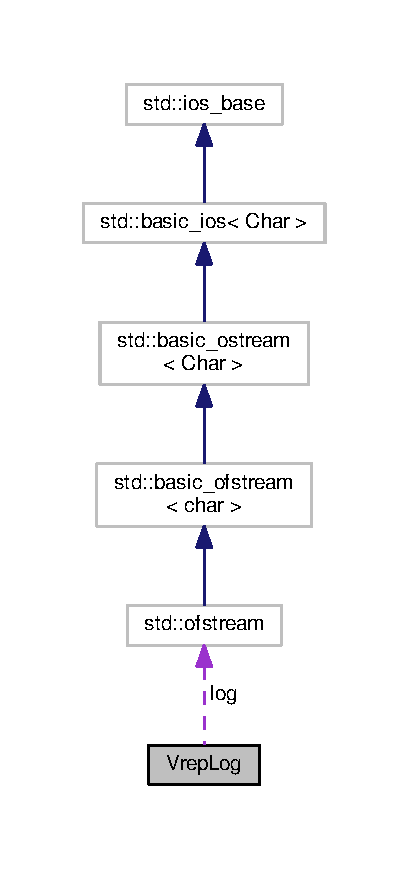
\includegraphics[width=196pt]{classVrepLog__coll__graph}
\end{center}
\end{figure}
\subsection*{Public Member Functions}
\begin{DoxyCompactItemize}
\item 
\hyperlink{classVrepLog_aa4e87cecbabab9b1eed0b42f97a56152}{Vrep\+Log} ()
\item 
{\footnotesize template$<$typename T $>$ }\\\hyperlink{classLogLine}{Log\+Line} \hyperlink{classVrepLog_a1a2744fc0ca891c3bf9767395791914b}{operator$<$$<$} (T \&t)
\end{DoxyCompactItemize}
\subsection*{Private Attributes}
\begin{DoxyCompactItemize}
\item 
std\+::ofstream \hyperlink{classVrepLog_a5c17a8191843eaf3d2743a84901d8e64}{log}
\end{DoxyCompactItemize}


\subsection{Detailed Description}
Class for creating a log file. 

\begin{DoxyRefDesc}{Todo}
\item[\hyperlink{todo__todo000004}{Todo}]cleanup code from superfluous debug logging \end{DoxyRefDesc}


\subsection{Constructor \& Destructor Documentation}
\index{Vrep\+Log@{Vrep\+Log}!Vrep\+Log@{Vrep\+Log}}
\index{Vrep\+Log@{Vrep\+Log}!Vrep\+Log@{Vrep\+Log}}
\subsubsection[{\texorpdfstring{Vrep\+Log()}{VrepLog()}}]{\setlength{\rightskip}{0pt plus 5cm}Vrep\+Log\+::\+Vrep\+Log (
\begin{DoxyParamCaption}
{}
\end{DoxyParamCaption}
)\hspace{0.3cm}{\ttfamily [inline]}}\hypertarget{classVrepLog_aa4e87cecbabab9b1eed0b42f97a56152}{}\label{classVrepLog_aa4e87cecbabab9b1eed0b42f97a56152}


\subsection{Member Function Documentation}
\index{Vrep\+Log@{Vrep\+Log}!operator$<$$<$@{operator$<$$<$}}
\index{operator$<$$<$@{operator$<$$<$}!Vrep\+Log@{Vrep\+Log}}
\subsubsection[{\texorpdfstring{operator$<$$<$(\+T \&t)}{operator<<(T &t)}}]{\setlength{\rightskip}{0pt plus 5cm}template$<$typename T $>$ {\bf Log\+Line} Vrep\+Log\+::operator$<$$<$ (
\begin{DoxyParamCaption}
\item[{T \&}]{t}
\end{DoxyParamCaption}
)\hspace{0.3cm}{\ttfamily [inline]}}\hypertarget{classVrepLog_a1a2744fc0ca891c3bf9767395791914b}{}\label{classVrepLog_a1a2744fc0ca891c3bf9767395791914b}


\subsection{Member Data Documentation}
\index{Vrep\+Log@{Vrep\+Log}!log@{log}}
\index{log@{log}!Vrep\+Log@{Vrep\+Log}}
\subsubsection[{\texorpdfstring{log}{log}}]{\setlength{\rightskip}{0pt plus 5cm}std\+::ofstream Vrep\+Log\+::log\hspace{0.3cm}{\ttfamily [private]}}\hypertarget{classVrepLog_a5c17a8191843eaf3d2743a84901d8e64}{}\label{classVrepLog_a5c17a8191843eaf3d2743a84901d8e64}


The documentation for this class was generated from the following file\+:\begin{DoxyCompactItemize}
\item 
\hyperlink{finken_8h}{finken.\+h}\end{DoxyCompactItemize}

\hypertarget{classVREPPlugin}{}\section{V\+R\+E\+P\+Plugin Class Reference}
\label{classVREPPlugin}\index{V\+R\+E\+P\+Plugin@{V\+R\+E\+P\+Plugin}}


Base vrepplugin class.  




{\ttfamily \#include $<$vrepplugin.\+h$>$}



Inheritance diagram for V\+R\+E\+P\+Plugin\+:\nopagebreak
\begin{figure}[H]
\begin{center}
\leavevmode
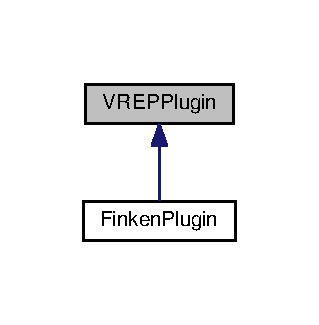
\includegraphics[width=153pt]{classVREPPlugin__inherit__graph}
\end{center}
\end{figure}


Collaboration diagram for V\+R\+E\+P\+Plugin\+:\nopagebreak
\begin{figure}[H]
\begin{center}
\leavevmode
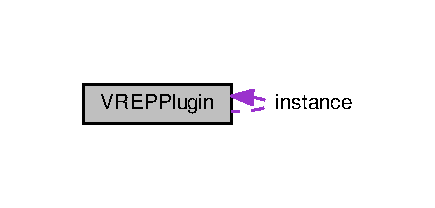
\includegraphics[width=209pt]{classVREPPlugin__coll__graph}
\end{center}
\end{figure}
\subsection*{Public Member Functions}
\begin{DoxyCompactItemize}
\item 
\hyperlink{classVREPPlugin_a5a2044c242eaa032a5608cd8c3b77fad}{V\+R\+E\+P\+Plugin} ()
\item 
virtual \hyperlink{classVREPPlugin_a73d3e01b6cb22ab256107eba5f97a08d}{$\sim$\+V\+R\+E\+P\+Plugin} ()
\item 
\hyperlink{classVREPPlugin}{V\+R\+E\+P\+Plugin} \& \hyperlink{classVREPPlugin_aac9c374d0718ea48d6ec5baa8d8ab2b2}{operator=} (const \hyperlink{classVREPPlugin}{V\+R\+E\+P\+Plugin} \&)=delete
\item 
\hyperlink{classVREPPlugin_accb66d8b1e8ded95475a15a3a42c9fbc}{V\+R\+E\+P\+Plugin} (const \hyperlink{classVREPPlugin}{V\+R\+E\+P\+Plugin} \&)=delete
\item 
virtual unsigned char \hyperlink{classVREPPlugin_ae5e6764e97874aa134447122bbadbf2a}{version} () const =0
\item 
virtual const std\+::string \hyperlink{classVREPPlugin_a345987cf0e2e8aa3af817cc0213e5c7a}{name} () const =0
\item 
virtual bool \hyperlink{classVREPPlugin_a4149b72b671ad72f63e9a75c58c0d628}{load} ()
\item 
virtual bool \hyperlink{classVREPPlugin_a49aff8a71c1c9f2af6e32b918eba99ff}{unload} ()
\item 
virtual void $\ast$ \hyperlink{classVREPPlugin_aae582606dda4aff564d102358b9af579}{refresh\+Dialog} (int $\ast$auxiliary\+Data, void $\ast$custom\+Data, int $\ast$reply\+Data)
\item 
virtual void $\ast$ \hyperlink{classVREPPlugin_a320dcb5ed4beaec82975be22b5c20e39}{menu\+Item\+Selected} (int $\ast$auxiliary\+Data, void $\ast$custom\+Data, int $\ast$reply\+Data)
\item 
virtual void $\ast$ \hyperlink{classVREPPlugin_a7df55bb967c9f217c77add60bb0d3868}{scene\+Content\+Change} (int $\ast$auxiliary\+Data, void $\ast$custom\+Data, int $\ast$reply\+Data)
\item 
virtual void $\ast$ \hyperlink{classVREPPlugin_affe1c1f37ffa8e04ea93e9eda9399402}{instance\+Pass} (int $\ast$auxiliary\+Data, void $\ast$custom\+Data, int $\ast$reply\+Data)
\item 
virtual void $\ast$ \hyperlink{classVREPPlugin_ae288b5fdec3fee292f23e61a021f4f5e}{instance\+Switch} (int $\ast$auxiliary\+Data, void $\ast$custom\+Data, int $\ast$reply\+Data)
\item 
virtual void $\ast$ \hyperlink{classVREPPlugin_a5aa8491d41b377e75917ab1273674f9f}{main\+Script\+Call} (int $\ast$auxiliary\+Data, void $\ast$custom\+Data, int $\ast$reply\+Data)
\item 
virtual void $\ast$ \hyperlink{classVREPPlugin_a58c9675c38c6ca1a75047864d3e4253c}{sim\+Start} (int $\ast$auxiliary\+Data, void $\ast$custom\+Data, int $\ast$reply\+Data)
\item 
virtual void $\ast$ \hyperlink{classVREPPlugin_a13ea56c8546d762468b21ebc141b4ca3}{sim\+End} (int $\ast$auxiliary\+Data, void $\ast$custom\+Data, int $\ast$reply\+Data)
\item 
virtual void $\ast$ \hyperlink{classVREPPlugin_a77e10632cbc7ae0581a151daea83ab1f}{scene\+Load} (int $\ast$auxiliary\+Data, void $\ast$custom\+Data, int $\ast$reply\+Data)
\item 
virtual void $\ast$ \hyperlink{classVREPPlugin_a40ededcae0889e8f8ecdf99d0f455179}{open} (int $\ast$auxiliary\+Data, void $\ast$custom\+Data, int $\ast$reply\+Data)
\item 
virtual void $\ast$ \hyperlink{classVREPPlugin_a048e1fbf7b4b5b7b96ea6ec132218e12}{action} (int $\ast$auxiliary\+Data, void $\ast$custom\+Data, int $\ast$reply\+Data)
\item 
virtual void $\ast$ \hyperlink{classVREPPlugin_af9fc2e6b9adf1436fc06e2555eaa3c2b}{close} (int $\ast$auxiliary\+Data, void $\ast$custom\+Data, int $\ast$reply\+Data)
\item 
virtual void $\ast$ \hyperlink{classVREPPlugin_af6a19ea1a3fbe91a86df1e92e6f623a2}{save} (int $\ast$auxiliary\+Data, void $\ast$custom\+Data, int $\ast$reply\+Data)
\item 
virtual void $\ast$ \hyperlink{classVREPPlugin_a3fce674766334a4ad6c63a179dff64ae}{render} (int $\ast$auxiliary\+Data, void $\ast$custom\+Data, int $\ast$reply\+Data)
\item 
virtual void $\ast$ \hyperlink{classVREPPlugin_aa04f0d2bb1b0d73a46a99e699e11830f}{broadcast} (int $\ast$auxiliary\+Data, void $\ast$custom\+Data, int $\ast$reply\+Data)
\item 
virtual void $\ast$ \hyperlink{classVREPPlugin_af3a92d9202afe61bf4979d0e24bd5425}{handle\+Other\+Message} (int message, int $\ast$auxiliary\+Data, void $\ast$custom\+Data, int $\ast$reply\+Data)
\end{DoxyCompactItemize}
\subsection*{Static Public Member Functions}
\begin{DoxyCompactItemize}
\item 
static \hyperlink{classVREPPlugin}{V\+R\+E\+P\+Plugin} \& \hyperlink{classVREPPlugin_a6c54bebcd2d0c09e7a20dd72ae82ec71}{get\+Instance} ()
\end{DoxyCompactItemize}
\subsection*{Static Private Attributes}
\begin{DoxyCompactItemize}
\item 
static \hyperlink{classVREPPlugin}{V\+R\+E\+P\+Plugin} $\ast$ \hyperlink{classVREPPlugin_abfc3869e912b4b01068c261003919415}{instance}
\end{DoxyCompactItemize}


\subsection{Detailed Description}
Base vrepplugin class. 

Finkenplugin inherits from this class 

\subsection{Constructor \& Destructor Documentation}
\index{V\+R\+E\+P\+Plugin@{V\+R\+E\+P\+Plugin}!V\+R\+E\+P\+Plugin@{V\+R\+E\+P\+Plugin}}
\index{V\+R\+E\+P\+Plugin@{V\+R\+E\+P\+Plugin}!V\+R\+E\+P\+Plugin@{V\+R\+E\+P\+Plugin}}
\subsubsection[{\texorpdfstring{V\+R\+E\+P\+Plugin()}{VREPPlugin()}}]{\setlength{\rightskip}{0pt plus 5cm}V\+R\+E\+P\+Plugin\+::\+V\+R\+E\+P\+Plugin (
\begin{DoxyParamCaption}
{}
\end{DoxyParamCaption}
)}\hypertarget{classVREPPlugin_a5a2044c242eaa032a5608cd8c3b77fad}{}\label{classVREPPlugin_a5a2044c242eaa032a5608cd8c3b77fad}
\index{V\+R\+E\+P\+Plugin@{V\+R\+E\+P\+Plugin}!````~V\+R\+E\+P\+Plugin@{$\sim$\+V\+R\+E\+P\+Plugin}}
\index{````~V\+R\+E\+P\+Plugin@{$\sim$\+V\+R\+E\+P\+Plugin}!V\+R\+E\+P\+Plugin@{V\+R\+E\+P\+Plugin}}
\subsubsection[{\texorpdfstring{$\sim$\+V\+R\+E\+P\+Plugin()}{~VREPPlugin()}}]{\setlength{\rightskip}{0pt plus 5cm}V\+R\+E\+P\+Plugin\+::$\sim$\+V\+R\+E\+P\+Plugin (
\begin{DoxyParamCaption}
{}
\end{DoxyParamCaption}
)\hspace{0.3cm}{\ttfamily [virtual]}}\hypertarget{classVREPPlugin_a73d3e01b6cb22ab256107eba5f97a08d}{}\label{classVREPPlugin_a73d3e01b6cb22ab256107eba5f97a08d}
\index{V\+R\+E\+P\+Plugin@{V\+R\+E\+P\+Plugin}!V\+R\+E\+P\+Plugin@{V\+R\+E\+P\+Plugin}}
\index{V\+R\+E\+P\+Plugin@{V\+R\+E\+P\+Plugin}!V\+R\+E\+P\+Plugin@{V\+R\+E\+P\+Plugin}}
\subsubsection[{\texorpdfstring{V\+R\+E\+P\+Plugin(const V\+R\+E\+P\+Plugin \&)=delete}{VREPPlugin(const VREPPlugin &)=delete}}]{\setlength{\rightskip}{0pt plus 5cm}V\+R\+E\+P\+Plugin\+::\+V\+R\+E\+P\+Plugin (
\begin{DoxyParamCaption}
\item[{const {\bf V\+R\+E\+P\+Plugin} \&}]{}
\end{DoxyParamCaption}
)\hspace{0.3cm}{\ttfamily [delete]}}\hypertarget{classVREPPlugin_accb66d8b1e8ded95475a15a3a42c9fbc}{}\label{classVREPPlugin_accb66d8b1e8ded95475a15a3a42c9fbc}


\subsection{Member Function Documentation}
\index{V\+R\+E\+P\+Plugin@{V\+R\+E\+P\+Plugin}!action@{action}}
\index{action@{action}!V\+R\+E\+P\+Plugin@{V\+R\+E\+P\+Plugin}}
\subsubsection[{\texorpdfstring{action(int $\ast$auxiliary\+Data, void $\ast$custom\+Data, int $\ast$reply\+Data)}{action(int *auxiliaryData, void *customData, int *replyData)}}]{\setlength{\rightskip}{0pt plus 5cm}void $\ast$ V\+R\+E\+P\+Plugin\+::action (
\begin{DoxyParamCaption}
\item[{int $\ast$}]{auxiliary\+Data, }
\item[{void $\ast$}]{custom\+Data, }
\item[{int $\ast$}]{reply\+Data}
\end{DoxyParamCaption}
)\hspace{0.3cm}{\ttfamily [virtual]}}\hypertarget{classVREPPlugin_a048e1fbf7b4b5b7b96ea6ec132218e12}{}\label{classVREPPlugin_a048e1fbf7b4b5b7b96ea6ec132218e12}


Reimplemented in \hyperlink{classFinkenPlugin_a00d8bcdd7c4b28eb76712b84f512b12b}{Finken\+Plugin}.



Here is the caller graph for this function\+:\nopagebreak
\begin{figure}[H]
\begin{center}
\leavevmode
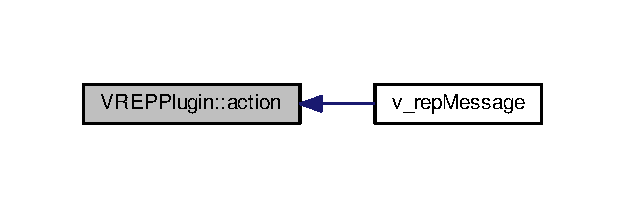
\includegraphics[width=300pt]{classVREPPlugin_a048e1fbf7b4b5b7b96ea6ec132218e12_icgraph}
\end{center}
\end{figure}


\index{V\+R\+E\+P\+Plugin@{V\+R\+E\+P\+Plugin}!broadcast@{broadcast}}
\index{broadcast@{broadcast}!V\+R\+E\+P\+Plugin@{V\+R\+E\+P\+Plugin}}
\subsubsection[{\texorpdfstring{broadcast(int $\ast$auxiliary\+Data, void $\ast$custom\+Data, int $\ast$reply\+Data)}{broadcast(int *auxiliaryData, void *customData, int *replyData)}}]{\setlength{\rightskip}{0pt plus 5cm}void $\ast$ V\+R\+E\+P\+Plugin\+::broadcast (
\begin{DoxyParamCaption}
\item[{int $\ast$}]{auxiliary\+Data, }
\item[{void $\ast$}]{custom\+Data, }
\item[{int $\ast$}]{reply\+Data}
\end{DoxyParamCaption}
)\hspace{0.3cm}{\ttfamily [virtual]}}\hypertarget{classVREPPlugin_aa04f0d2bb1b0d73a46a99e699e11830f}{}\label{classVREPPlugin_aa04f0d2bb1b0d73a46a99e699e11830f}


Here is the caller graph for this function\+:\nopagebreak
\begin{figure}[H]
\begin{center}
\leavevmode
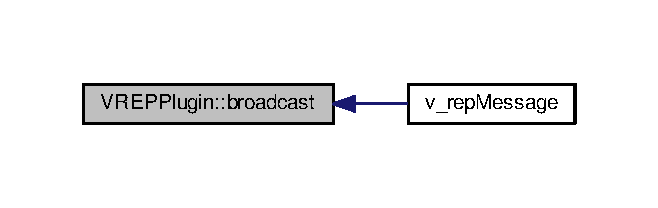
\includegraphics[width=316pt]{classVREPPlugin_aa04f0d2bb1b0d73a46a99e699e11830f_icgraph}
\end{center}
\end{figure}


\index{V\+R\+E\+P\+Plugin@{V\+R\+E\+P\+Plugin}!close@{close}}
\index{close@{close}!V\+R\+E\+P\+Plugin@{V\+R\+E\+P\+Plugin}}
\subsubsection[{\texorpdfstring{close(int $\ast$auxiliary\+Data, void $\ast$custom\+Data, int $\ast$reply\+Data)}{close(int *auxiliaryData, void *customData, int *replyData)}}]{\setlength{\rightskip}{0pt plus 5cm}void $\ast$ V\+R\+E\+P\+Plugin\+::close (
\begin{DoxyParamCaption}
\item[{int $\ast$}]{auxiliary\+Data, }
\item[{void $\ast$}]{custom\+Data, }
\item[{int $\ast$}]{reply\+Data}
\end{DoxyParamCaption}
)\hspace{0.3cm}{\ttfamily [virtual]}}\hypertarget{classVREPPlugin_af9fc2e6b9adf1436fc06e2555eaa3c2b}{}\label{classVREPPlugin_af9fc2e6b9adf1436fc06e2555eaa3c2b}


Here is the caller graph for this function\+:\nopagebreak
\begin{figure}[H]
\begin{center}
\leavevmode
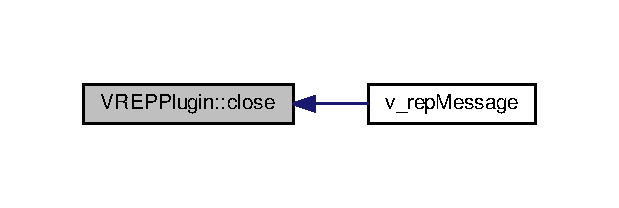
\includegraphics[width=297pt]{classVREPPlugin_af9fc2e6b9adf1436fc06e2555eaa3c2b_icgraph}
\end{center}
\end{figure}


\index{V\+R\+E\+P\+Plugin@{V\+R\+E\+P\+Plugin}!get\+Instance@{get\+Instance}}
\index{get\+Instance@{get\+Instance}!V\+R\+E\+P\+Plugin@{V\+R\+E\+P\+Plugin}}
\subsubsection[{\texorpdfstring{get\+Instance()}{getInstance()}}]{\setlength{\rightskip}{0pt plus 5cm}{\bf V\+R\+E\+P\+Plugin} \& V\+R\+E\+P\+Plugin\+::get\+Instance (
\begin{DoxyParamCaption}
{}
\end{DoxyParamCaption}
)\hspace{0.3cm}{\ttfamily [static]}}\hypertarget{classVREPPlugin_a6c54bebcd2d0c09e7a20dd72ae82ec71}{}\label{classVREPPlugin_a6c54bebcd2d0c09e7a20dd72ae82ec71}


Here is the caller graph for this function\+:\nopagebreak
\begin{figure}[H]
\begin{center}
\leavevmode
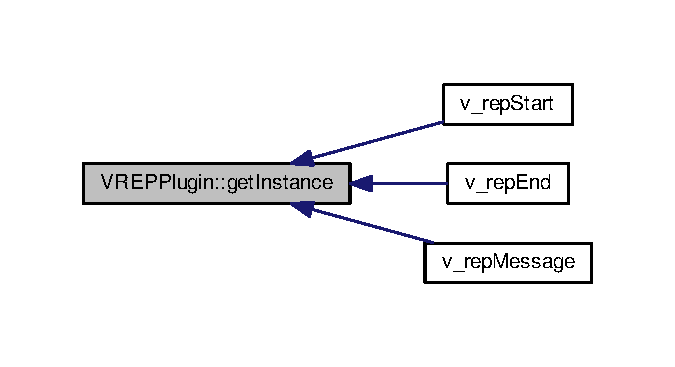
\includegraphics[width=324pt]{classVREPPlugin_a6c54bebcd2d0c09e7a20dd72ae82ec71_icgraph}
\end{center}
\end{figure}


\index{V\+R\+E\+P\+Plugin@{V\+R\+E\+P\+Plugin}!handle\+Other\+Message@{handle\+Other\+Message}}
\index{handle\+Other\+Message@{handle\+Other\+Message}!V\+R\+E\+P\+Plugin@{V\+R\+E\+P\+Plugin}}
\subsubsection[{\texorpdfstring{handle\+Other\+Message(int message, int $\ast$auxiliary\+Data, void $\ast$custom\+Data, int $\ast$reply\+Data)}{handleOtherMessage(int message, int *auxiliaryData, void *customData, int *replyData)}}]{\setlength{\rightskip}{0pt plus 5cm}void $\ast$ V\+R\+E\+P\+Plugin\+::handle\+Other\+Message (
\begin{DoxyParamCaption}
\item[{int}]{message, }
\item[{int $\ast$}]{auxiliary\+Data, }
\item[{void $\ast$}]{custom\+Data, }
\item[{int $\ast$}]{reply\+Data}
\end{DoxyParamCaption}
)\hspace{0.3cm}{\ttfamily [virtual]}}\hypertarget{classVREPPlugin_af3a92d9202afe61bf4979d0e24bd5425}{}\label{classVREPPlugin_af3a92d9202afe61bf4979d0e24bd5425}


Here is the caller graph for this function\+:\nopagebreak
\begin{figure}[H]
\begin{center}
\leavevmode
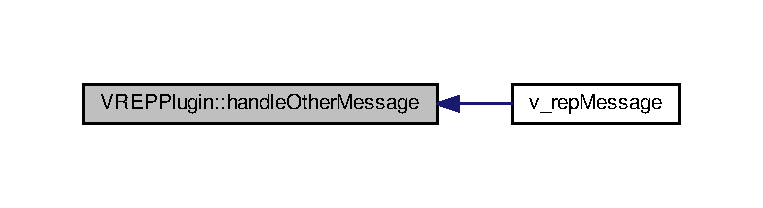
\includegraphics[width=350pt]{classVREPPlugin_af3a92d9202afe61bf4979d0e24bd5425_icgraph}
\end{center}
\end{figure}


\index{V\+R\+E\+P\+Plugin@{V\+R\+E\+P\+Plugin}!instance\+Pass@{instance\+Pass}}
\index{instance\+Pass@{instance\+Pass}!V\+R\+E\+P\+Plugin@{V\+R\+E\+P\+Plugin}}
\subsubsection[{\texorpdfstring{instance\+Pass(int $\ast$auxiliary\+Data, void $\ast$custom\+Data, int $\ast$reply\+Data)}{instancePass(int *auxiliaryData, void *customData, int *replyData)}}]{\setlength{\rightskip}{0pt plus 5cm}void $\ast$ V\+R\+E\+P\+Plugin\+::instance\+Pass (
\begin{DoxyParamCaption}
\item[{int $\ast$}]{auxiliary\+Data, }
\item[{void $\ast$}]{custom\+Data, }
\item[{int $\ast$}]{reply\+Data}
\end{DoxyParamCaption}
)\hspace{0.3cm}{\ttfamily [virtual]}}\hypertarget{classVREPPlugin_affe1c1f37ffa8e04ea93e9eda9399402}{}\label{classVREPPlugin_affe1c1f37ffa8e04ea93e9eda9399402}


Here is the caller graph for this function\+:\nopagebreak
\begin{figure}[H]
\begin{center}
\leavevmode
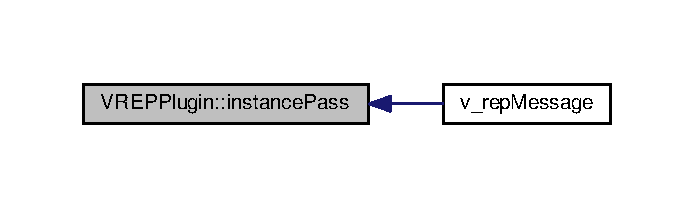
\includegraphics[width=333pt]{classVREPPlugin_affe1c1f37ffa8e04ea93e9eda9399402_icgraph}
\end{center}
\end{figure}


\index{V\+R\+E\+P\+Plugin@{V\+R\+E\+P\+Plugin}!instance\+Switch@{instance\+Switch}}
\index{instance\+Switch@{instance\+Switch}!V\+R\+E\+P\+Plugin@{V\+R\+E\+P\+Plugin}}
\subsubsection[{\texorpdfstring{instance\+Switch(int $\ast$auxiliary\+Data, void $\ast$custom\+Data, int $\ast$reply\+Data)}{instanceSwitch(int *auxiliaryData, void *customData, int *replyData)}}]{\setlength{\rightskip}{0pt plus 5cm}void $\ast$ V\+R\+E\+P\+Plugin\+::instance\+Switch (
\begin{DoxyParamCaption}
\item[{int $\ast$}]{auxiliary\+Data, }
\item[{void $\ast$}]{custom\+Data, }
\item[{int $\ast$}]{reply\+Data}
\end{DoxyParamCaption}
)\hspace{0.3cm}{\ttfamily [virtual]}}\hypertarget{classVREPPlugin_ae288b5fdec3fee292f23e61a021f4f5e}{}\label{classVREPPlugin_ae288b5fdec3fee292f23e61a021f4f5e}


Here is the caller graph for this function\+:\nopagebreak
\begin{figure}[H]
\begin{center}
\leavevmode
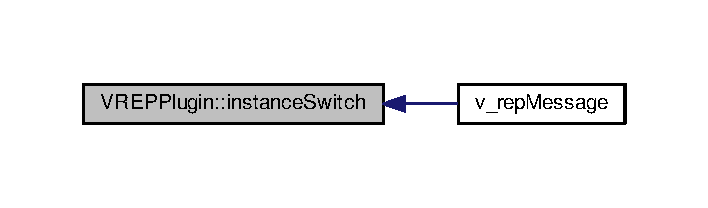
\includegraphics[width=340pt]{classVREPPlugin_ae288b5fdec3fee292f23e61a021f4f5e_icgraph}
\end{center}
\end{figure}


\index{V\+R\+E\+P\+Plugin@{V\+R\+E\+P\+Plugin}!load@{load}}
\index{load@{load}!V\+R\+E\+P\+Plugin@{V\+R\+E\+P\+Plugin}}
\subsubsection[{\texorpdfstring{load()}{load()}}]{\setlength{\rightskip}{0pt plus 5cm}bool V\+R\+E\+P\+Plugin\+::load (
\begin{DoxyParamCaption}
{}
\end{DoxyParamCaption}
)\hspace{0.3cm}{\ttfamily [virtual]}}\hypertarget{classVREPPlugin_a4149b72b671ad72f63e9a75c58c0d628}{}\label{classVREPPlugin_a4149b72b671ad72f63e9a75c58c0d628}


Reimplemented in \hyperlink{classFinkenPlugin_afbe5d82635afe4b0c407de4724e8ee14}{Finken\+Plugin}.



Here is the caller graph for this function\+:\nopagebreak
\begin{figure}[H]
\begin{center}
\leavevmode
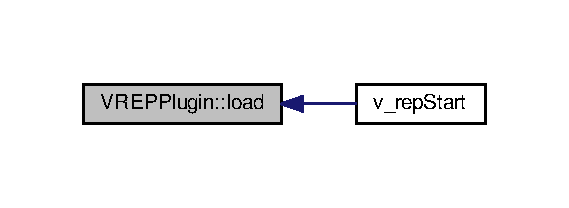
\includegraphics[width=273pt]{classVREPPlugin_a4149b72b671ad72f63e9a75c58c0d628_icgraph}
\end{center}
\end{figure}


\index{V\+R\+E\+P\+Plugin@{V\+R\+E\+P\+Plugin}!main\+Script\+Call@{main\+Script\+Call}}
\index{main\+Script\+Call@{main\+Script\+Call}!V\+R\+E\+P\+Plugin@{V\+R\+E\+P\+Plugin}}
\subsubsection[{\texorpdfstring{main\+Script\+Call(int $\ast$auxiliary\+Data, void $\ast$custom\+Data, int $\ast$reply\+Data)}{mainScriptCall(int *auxiliaryData, void *customData, int *replyData)}}]{\setlength{\rightskip}{0pt plus 5cm}void $\ast$ V\+R\+E\+P\+Plugin\+::main\+Script\+Call (
\begin{DoxyParamCaption}
\item[{int $\ast$}]{auxiliary\+Data, }
\item[{void $\ast$}]{custom\+Data, }
\item[{int $\ast$}]{reply\+Data}
\end{DoxyParamCaption}
)\hspace{0.3cm}{\ttfamily [virtual]}}\hypertarget{classVREPPlugin_a5aa8491d41b377e75917ab1273674f9f}{}\label{classVREPPlugin_a5aa8491d41b377e75917ab1273674f9f}


Here is the caller graph for this function\+:\nopagebreak
\begin{figure}[H]
\begin{center}
\leavevmode
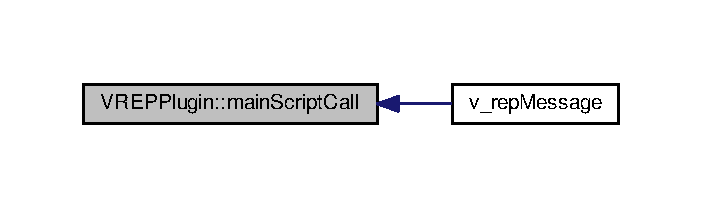
\includegraphics[width=337pt]{classVREPPlugin_a5aa8491d41b377e75917ab1273674f9f_icgraph}
\end{center}
\end{figure}


\index{V\+R\+E\+P\+Plugin@{V\+R\+E\+P\+Plugin}!menu\+Item\+Selected@{menu\+Item\+Selected}}
\index{menu\+Item\+Selected@{menu\+Item\+Selected}!V\+R\+E\+P\+Plugin@{V\+R\+E\+P\+Plugin}}
\subsubsection[{\texorpdfstring{menu\+Item\+Selected(int $\ast$auxiliary\+Data, void $\ast$custom\+Data, int $\ast$reply\+Data)}{menuItemSelected(int *auxiliaryData, void *customData, int *replyData)}}]{\setlength{\rightskip}{0pt plus 5cm}void $\ast$ V\+R\+E\+P\+Plugin\+::menu\+Item\+Selected (
\begin{DoxyParamCaption}
\item[{int $\ast$}]{auxiliary\+Data, }
\item[{void $\ast$}]{custom\+Data, }
\item[{int $\ast$}]{reply\+Data}
\end{DoxyParamCaption}
)\hspace{0.3cm}{\ttfamily [virtual]}}\hypertarget{classVREPPlugin_a320dcb5ed4beaec82975be22b5c20e39}{}\label{classVREPPlugin_a320dcb5ed4beaec82975be22b5c20e39}


Here is the caller graph for this function\+:\nopagebreak
\begin{figure}[H]
\begin{center}
\leavevmode
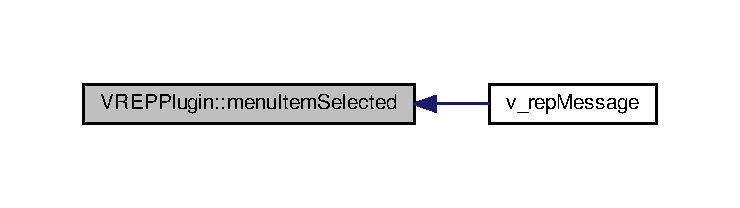
\includegraphics[width=350pt]{classVREPPlugin_a320dcb5ed4beaec82975be22b5c20e39_icgraph}
\end{center}
\end{figure}


\index{V\+R\+E\+P\+Plugin@{V\+R\+E\+P\+Plugin}!name@{name}}
\index{name@{name}!V\+R\+E\+P\+Plugin@{V\+R\+E\+P\+Plugin}}
\subsubsection[{\texorpdfstring{name() const =0}{name() const =0}}]{\setlength{\rightskip}{0pt plus 5cm}virtual const std\+::string V\+R\+E\+P\+Plugin\+::name (
\begin{DoxyParamCaption}
{}
\end{DoxyParamCaption}
) const\hspace{0.3cm}{\ttfamily [pure virtual]}}\hypertarget{classVREPPlugin_a345987cf0e2e8aa3af817cc0213e5c7a}{}\label{classVREPPlugin_a345987cf0e2e8aa3af817cc0213e5c7a}


Implemented in \hyperlink{classFinkenPlugin_a1a7d0d65f88654c37b282e07d36417ec}{Finken\+Plugin}.



Here is the caller graph for this function\+:\nopagebreak
\begin{figure}[H]
\begin{center}
\leavevmode
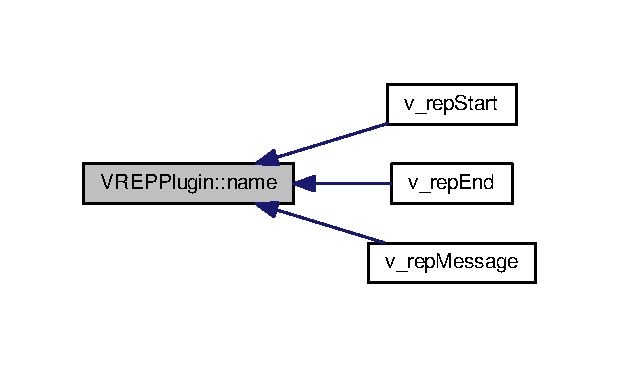
\includegraphics[width=297pt]{classVREPPlugin_a345987cf0e2e8aa3af817cc0213e5c7a_icgraph}
\end{center}
\end{figure}


\index{V\+R\+E\+P\+Plugin@{V\+R\+E\+P\+Plugin}!open@{open}}
\index{open@{open}!V\+R\+E\+P\+Plugin@{V\+R\+E\+P\+Plugin}}
\subsubsection[{\texorpdfstring{open(int $\ast$auxiliary\+Data, void $\ast$custom\+Data, int $\ast$reply\+Data)}{open(int *auxiliaryData, void *customData, int *replyData)}}]{\setlength{\rightskip}{0pt plus 5cm}void $\ast$ V\+R\+E\+P\+Plugin\+::open (
\begin{DoxyParamCaption}
\item[{int $\ast$}]{auxiliary\+Data, }
\item[{void $\ast$}]{custom\+Data, }
\item[{int $\ast$}]{reply\+Data}
\end{DoxyParamCaption}
)\hspace{0.3cm}{\ttfamily [virtual]}}\hypertarget{classVREPPlugin_a40ededcae0889e8f8ecdf99d0f455179}{}\label{classVREPPlugin_a40ededcae0889e8f8ecdf99d0f455179}


Here is the caller graph for this function\+:\nopagebreak
\begin{figure}[H]
\begin{center}
\leavevmode
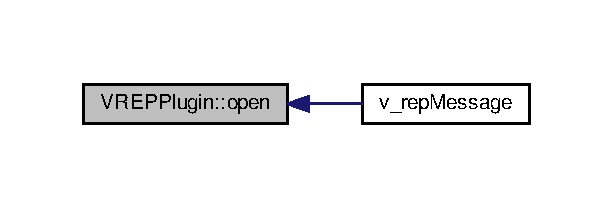
\includegraphics[width=294pt]{classVREPPlugin_a40ededcae0889e8f8ecdf99d0f455179_icgraph}
\end{center}
\end{figure}


\index{V\+R\+E\+P\+Plugin@{V\+R\+E\+P\+Plugin}!operator=@{operator=}}
\index{operator=@{operator=}!V\+R\+E\+P\+Plugin@{V\+R\+E\+P\+Plugin}}
\subsubsection[{\texorpdfstring{operator=(const V\+R\+E\+P\+Plugin \&)=delete}{operator=(const VREPPlugin &)=delete}}]{\setlength{\rightskip}{0pt plus 5cm}{\bf V\+R\+E\+P\+Plugin}\& V\+R\+E\+P\+Plugin\+::operator= (
\begin{DoxyParamCaption}
\item[{const {\bf V\+R\+E\+P\+Plugin} \&}]{}
\end{DoxyParamCaption}
)\hspace{0.3cm}{\ttfamily [delete]}}\hypertarget{classVREPPlugin_aac9c374d0718ea48d6ec5baa8d8ab2b2}{}\label{classVREPPlugin_aac9c374d0718ea48d6ec5baa8d8ab2b2}
\index{V\+R\+E\+P\+Plugin@{V\+R\+E\+P\+Plugin}!refresh\+Dialog@{refresh\+Dialog}}
\index{refresh\+Dialog@{refresh\+Dialog}!V\+R\+E\+P\+Plugin@{V\+R\+E\+P\+Plugin}}
\subsubsection[{\texorpdfstring{refresh\+Dialog(int $\ast$auxiliary\+Data, void $\ast$custom\+Data, int $\ast$reply\+Data)}{refreshDialog(int *auxiliaryData, void *customData, int *replyData)}}]{\setlength{\rightskip}{0pt plus 5cm}void $\ast$ V\+R\+E\+P\+Plugin\+::refresh\+Dialog (
\begin{DoxyParamCaption}
\item[{int $\ast$}]{auxiliary\+Data, }
\item[{void $\ast$}]{custom\+Data, }
\item[{int $\ast$}]{reply\+Data}
\end{DoxyParamCaption}
)\hspace{0.3cm}{\ttfamily [virtual]}}\hypertarget{classVREPPlugin_aae582606dda4aff564d102358b9af579}{}\label{classVREPPlugin_aae582606dda4aff564d102358b9af579}


Here is the caller graph for this function\+:\nopagebreak
\begin{figure}[H]
\begin{center}
\leavevmode
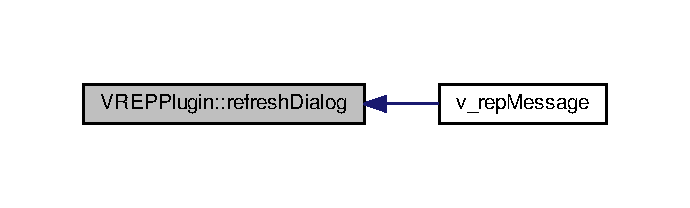
\includegraphics[width=331pt]{classVREPPlugin_aae582606dda4aff564d102358b9af579_icgraph}
\end{center}
\end{figure}


\index{V\+R\+E\+P\+Plugin@{V\+R\+E\+P\+Plugin}!render@{render}}
\index{render@{render}!V\+R\+E\+P\+Plugin@{V\+R\+E\+P\+Plugin}}
\subsubsection[{\texorpdfstring{render(int $\ast$auxiliary\+Data, void $\ast$custom\+Data, int $\ast$reply\+Data)}{render(int *auxiliaryData, void *customData, int *replyData)}}]{\setlength{\rightskip}{0pt plus 5cm}void $\ast$ V\+R\+E\+P\+Plugin\+::render (
\begin{DoxyParamCaption}
\item[{int $\ast$}]{auxiliary\+Data, }
\item[{void $\ast$}]{custom\+Data, }
\item[{int $\ast$}]{reply\+Data}
\end{DoxyParamCaption}
)\hspace{0.3cm}{\ttfamily [virtual]}}\hypertarget{classVREPPlugin_a3fce674766334a4ad6c63a179dff64ae}{}\label{classVREPPlugin_a3fce674766334a4ad6c63a179dff64ae}


Here is the caller graph for this function\+:\nopagebreak
\begin{figure}[H]
\begin{center}
\leavevmode
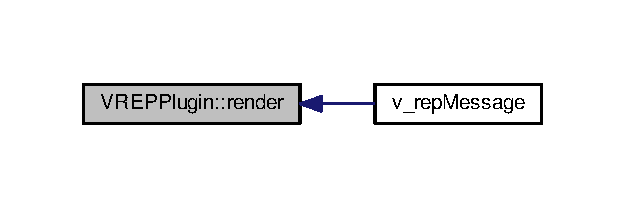
\includegraphics[width=300pt]{classVREPPlugin_a3fce674766334a4ad6c63a179dff64ae_icgraph}
\end{center}
\end{figure}


\index{V\+R\+E\+P\+Plugin@{V\+R\+E\+P\+Plugin}!save@{save}}
\index{save@{save}!V\+R\+E\+P\+Plugin@{V\+R\+E\+P\+Plugin}}
\subsubsection[{\texorpdfstring{save(int $\ast$auxiliary\+Data, void $\ast$custom\+Data, int $\ast$reply\+Data)}{save(int *auxiliaryData, void *customData, int *replyData)}}]{\setlength{\rightskip}{0pt plus 5cm}void $\ast$ V\+R\+E\+P\+Plugin\+::save (
\begin{DoxyParamCaption}
\item[{int $\ast$}]{auxiliary\+Data, }
\item[{void $\ast$}]{custom\+Data, }
\item[{int $\ast$}]{reply\+Data}
\end{DoxyParamCaption}
)\hspace{0.3cm}{\ttfamily [virtual]}}\hypertarget{classVREPPlugin_af6a19ea1a3fbe91a86df1e92e6f623a2}{}\label{classVREPPlugin_af6a19ea1a3fbe91a86df1e92e6f623a2}


Here is the caller graph for this function\+:\nopagebreak
\begin{figure}[H]
\begin{center}
\leavevmode
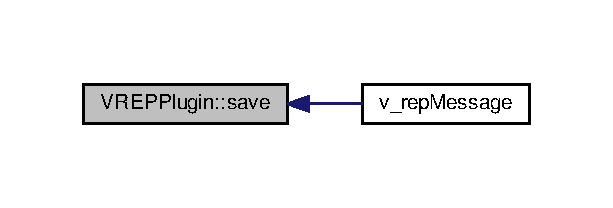
\includegraphics[width=294pt]{classVREPPlugin_af6a19ea1a3fbe91a86df1e92e6f623a2_icgraph}
\end{center}
\end{figure}


\index{V\+R\+E\+P\+Plugin@{V\+R\+E\+P\+Plugin}!scene\+Content\+Change@{scene\+Content\+Change}}
\index{scene\+Content\+Change@{scene\+Content\+Change}!V\+R\+E\+P\+Plugin@{V\+R\+E\+P\+Plugin}}
\subsubsection[{\texorpdfstring{scene\+Content\+Change(int $\ast$auxiliary\+Data, void $\ast$custom\+Data, int $\ast$reply\+Data)}{sceneContentChange(int *auxiliaryData, void *customData, int *replyData)}}]{\setlength{\rightskip}{0pt plus 5cm}void $\ast$ V\+R\+E\+P\+Plugin\+::scene\+Content\+Change (
\begin{DoxyParamCaption}
\item[{int $\ast$}]{auxiliary\+Data, }
\item[{void $\ast$}]{custom\+Data, }
\item[{int $\ast$}]{reply\+Data}
\end{DoxyParamCaption}
)\hspace{0.3cm}{\ttfamily [virtual]}}\hypertarget{classVREPPlugin_a7df55bb967c9f217c77add60bb0d3868}{}\label{classVREPPlugin_a7df55bb967c9f217c77add60bb0d3868}


Here is the caller graph for this function\+:\nopagebreak
\begin{figure}[H]
\begin{center}
\leavevmode
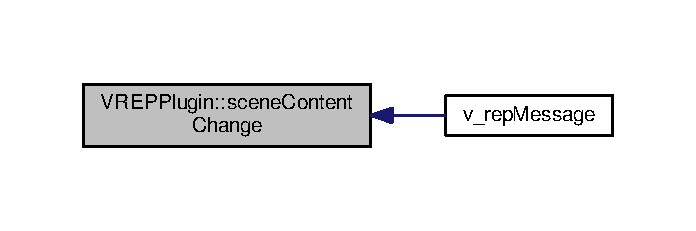
\includegraphics[width=334pt]{classVREPPlugin_a7df55bb967c9f217c77add60bb0d3868_icgraph}
\end{center}
\end{figure}


\index{V\+R\+E\+P\+Plugin@{V\+R\+E\+P\+Plugin}!scene\+Load@{scene\+Load}}
\index{scene\+Load@{scene\+Load}!V\+R\+E\+P\+Plugin@{V\+R\+E\+P\+Plugin}}
\subsubsection[{\texorpdfstring{scene\+Load(int $\ast$auxiliary\+Data, void $\ast$custom\+Data, int $\ast$reply\+Data)}{sceneLoad(int *auxiliaryData, void *customData, int *replyData)}}]{\setlength{\rightskip}{0pt plus 5cm}void $\ast$ V\+R\+E\+P\+Plugin\+::scene\+Load (
\begin{DoxyParamCaption}
\item[{int $\ast$}]{auxiliary\+Data, }
\item[{void $\ast$}]{custom\+Data, }
\item[{int $\ast$}]{reply\+Data}
\end{DoxyParamCaption}
)\hspace{0.3cm}{\ttfamily [virtual]}}\hypertarget{classVREPPlugin_a77e10632cbc7ae0581a151daea83ab1f}{}\label{classVREPPlugin_a77e10632cbc7ae0581a151daea83ab1f}


Reimplemented in \hyperlink{classFinkenPlugin_a82c0cd5fa1b9fdb5f5a625458a9b545b}{Finken\+Plugin}.



Here is the caller graph for this function\+:\nopagebreak
\begin{figure}[H]
\begin{center}
\leavevmode
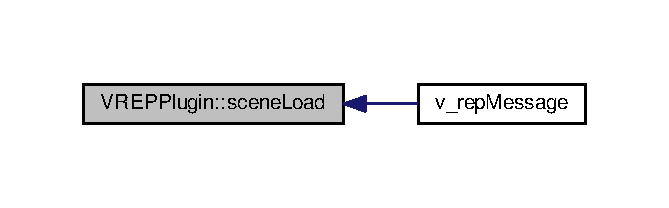
\includegraphics[width=321pt]{classVREPPlugin_a77e10632cbc7ae0581a151daea83ab1f_icgraph}
\end{center}
\end{figure}


\index{V\+R\+E\+P\+Plugin@{V\+R\+E\+P\+Plugin}!sim\+End@{sim\+End}}
\index{sim\+End@{sim\+End}!V\+R\+E\+P\+Plugin@{V\+R\+E\+P\+Plugin}}
\subsubsection[{\texorpdfstring{sim\+End(int $\ast$auxiliary\+Data, void $\ast$custom\+Data, int $\ast$reply\+Data)}{simEnd(int *auxiliaryData, void *customData, int *replyData)}}]{\setlength{\rightskip}{0pt plus 5cm}void $\ast$ V\+R\+E\+P\+Plugin\+::sim\+End (
\begin{DoxyParamCaption}
\item[{int $\ast$}]{auxiliary\+Data, }
\item[{void $\ast$}]{custom\+Data, }
\item[{int $\ast$}]{reply\+Data}
\end{DoxyParamCaption}
)\hspace{0.3cm}{\ttfamily [virtual]}}\hypertarget{classVREPPlugin_a13ea56c8546d762468b21ebc141b4ca3}{}\label{classVREPPlugin_a13ea56c8546d762468b21ebc141b4ca3}


Reimplemented in \hyperlink{classFinkenPlugin_aec5f5cf14ca485055ccc321a716780a4}{Finken\+Plugin}.



Here is the caller graph for this function\+:\nopagebreak
\begin{figure}[H]
\begin{center}
\leavevmode
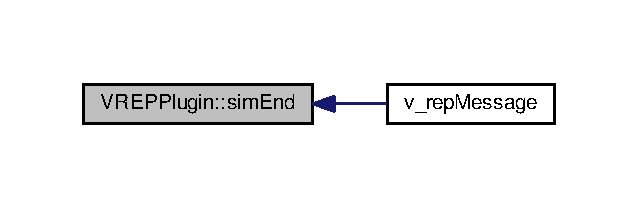
\includegraphics[width=306pt]{classVREPPlugin_a13ea56c8546d762468b21ebc141b4ca3_icgraph}
\end{center}
\end{figure}


\index{V\+R\+E\+P\+Plugin@{V\+R\+E\+P\+Plugin}!sim\+Start@{sim\+Start}}
\index{sim\+Start@{sim\+Start}!V\+R\+E\+P\+Plugin@{V\+R\+E\+P\+Plugin}}
\subsubsection[{\texorpdfstring{sim\+Start(int $\ast$auxiliary\+Data, void $\ast$custom\+Data, int $\ast$reply\+Data)}{simStart(int *auxiliaryData, void *customData, int *replyData)}}]{\setlength{\rightskip}{0pt plus 5cm}void $\ast$ V\+R\+E\+P\+Plugin\+::sim\+Start (
\begin{DoxyParamCaption}
\item[{int $\ast$}]{auxiliary\+Data, }
\item[{void $\ast$}]{custom\+Data, }
\item[{int $\ast$}]{reply\+Data}
\end{DoxyParamCaption}
)\hspace{0.3cm}{\ttfamily [virtual]}}\hypertarget{classVREPPlugin_a58c9675c38c6ca1a75047864d3e4253c}{}\label{classVREPPlugin_a58c9675c38c6ca1a75047864d3e4253c}


Reimplemented in \hyperlink{classFinkenPlugin_a142f62305fcc926bb6cf86744edbb82b}{Finken\+Plugin}.



Here is the caller graph for this function\+:\nopagebreak
\begin{figure}[H]
\begin{center}
\leavevmode
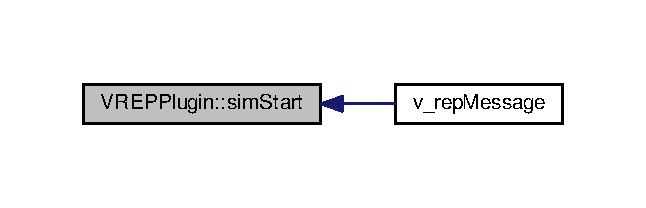
\includegraphics[width=310pt]{classVREPPlugin_a58c9675c38c6ca1a75047864d3e4253c_icgraph}
\end{center}
\end{figure}


\index{V\+R\+E\+P\+Plugin@{V\+R\+E\+P\+Plugin}!unload@{unload}}
\index{unload@{unload}!V\+R\+E\+P\+Plugin@{V\+R\+E\+P\+Plugin}}
\subsubsection[{\texorpdfstring{unload()}{unload()}}]{\setlength{\rightskip}{0pt plus 5cm}bool V\+R\+E\+P\+Plugin\+::unload (
\begin{DoxyParamCaption}
{}
\end{DoxyParamCaption}
)\hspace{0.3cm}{\ttfamily [virtual]}}\hypertarget{classVREPPlugin_a49aff8a71c1c9f2af6e32b918eba99ff}{}\label{classVREPPlugin_a49aff8a71c1c9f2af6e32b918eba99ff}


Reimplemented in \hyperlink{classFinkenPlugin_ae9c984b362c6a828206fa6201291851c}{Finken\+Plugin}.



Here is the caller graph for this function\+:\nopagebreak
\begin{figure}[H]
\begin{center}
\leavevmode
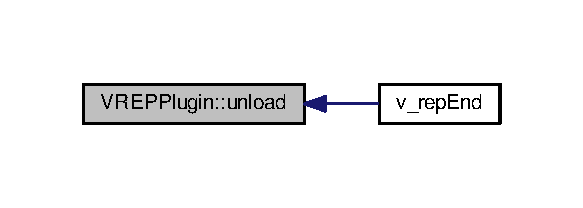
\includegraphics[width=280pt]{classVREPPlugin_a49aff8a71c1c9f2af6e32b918eba99ff_icgraph}
\end{center}
\end{figure}


\index{V\+R\+E\+P\+Plugin@{V\+R\+E\+P\+Plugin}!version@{version}}
\index{version@{version}!V\+R\+E\+P\+Plugin@{V\+R\+E\+P\+Plugin}}
\subsubsection[{\texorpdfstring{version() const =0}{version() const =0}}]{\setlength{\rightskip}{0pt plus 5cm}virtual unsigned char V\+R\+E\+P\+Plugin\+::version (
\begin{DoxyParamCaption}
{}
\end{DoxyParamCaption}
) const\hspace{0.3cm}{\ttfamily [pure virtual]}}\hypertarget{classVREPPlugin_ae5e6764e97874aa134447122bbadbf2a}{}\label{classVREPPlugin_ae5e6764e97874aa134447122bbadbf2a}


Implemented in \hyperlink{classFinkenPlugin_a046a229dfbc8185bac916ad2e49ec865}{Finken\+Plugin}.



Here is the caller graph for this function\+:\nopagebreak
\begin{figure}[H]
\begin{center}
\leavevmode
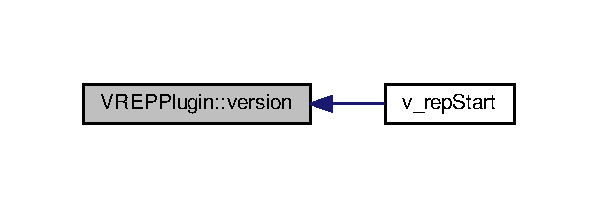
\includegraphics[width=287pt]{classVREPPlugin_ae5e6764e97874aa134447122bbadbf2a_icgraph}
\end{center}
\end{figure}




\subsection{Member Data Documentation}
\index{V\+R\+E\+P\+Plugin@{V\+R\+E\+P\+Plugin}!instance@{instance}}
\index{instance@{instance}!V\+R\+E\+P\+Plugin@{V\+R\+E\+P\+Plugin}}
\subsubsection[{\texorpdfstring{instance}{instance}}]{\setlength{\rightskip}{0pt plus 5cm}{\bf V\+R\+E\+P\+Plugin} $\ast$ V\+R\+E\+P\+Plugin\+::instance\hspace{0.3cm}{\ttfamily [static]}, {\ttfamily [private]}}\hypertarget{classVREPPlugin_abfc3869e912b4b01068c261003919415}{}\label{classVREPPlugin_abfc3869e912b4b01068c261003919415}


The documentation for this class was generated from the following files\+:\begin{DoxyCompactItemize}
\item 
\hyperlink{vrepplugin_8h}{vrepplugin.\+h}\item 
\hyperlink{vrepplugin_8cpp}{vrepplugin.\+cpp}\end{DoxyCompactItemize}

\chapter{File Documentation}
\hypertarget{attitudesensor_8cpp}{}\section{attitudesensor.\+cpp File Reference}
\label{attitudesensor_8cpp}\index{attitudesensor.\+cpp@{attitudesensor.\+cpp}}
{\ttfamily \#include \char`\"{}attitudesensor.\+h\char`\"{}}\\*
{\ttfamily \#include \char`\"{}v\+\_\+rep\+Lib.\+h\char`\"{}}\\*
{\ttfamily \#include $<$iostream$>$}\\*
{\ttfamily \#include $<$vector$>$}\\*
Include dependency graph for attitudesensor.\+cpp\+:

\hypertarget{attitudesensor_8h}{}\section{attitudesensor.\+h File Reference}
\label{attitudesensor_8h}\index{attitudesensor.\+h@{attitudesensor.\+h}}
{\ttfamily \#include \char`\"{}sensor.\+h\char`\"{}}\\*
Include dependency graph for attitudesensor.\+h\+:\nopagebreak
\begin{figure}[H]
\begin{center}
\leavevmode
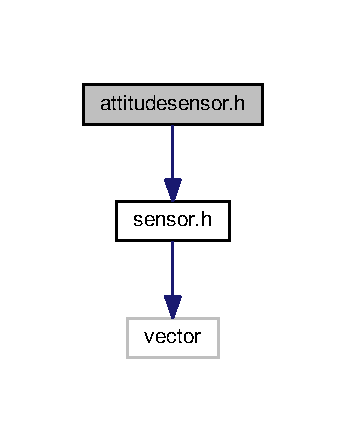
\includegraphics[width=166pt]{attitudesensor_8h__incl}
\end{center}
\end{figure}
This graph shows which files directly or indirectly include this file\+:\nopagebreak
\begin{figure}[H]
\begin{center}
\leavevmode
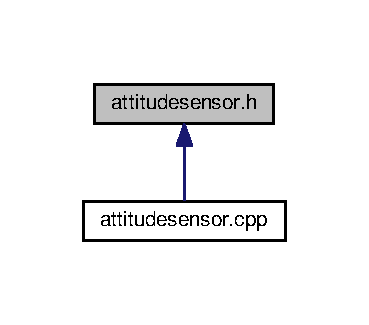
\includegraphics[width=177pt]{attitudesensor_8h__dep__incl}
\end{center}
\end{figure}
\subsection*{Classes}
\begin{DoxyCompactItemize}
\item 
class \hyperlink{classAttitudeSensor}{Attitude\+Sensor}
\begin{DoxyCompactList}\small\item\em Currently unused class for an attitude sensor. \end{DoxyCompactList}\end{DoxyCompactItemize}

\hypertarget{finken_8cpp}{}\section{finken.\+cpp File Reference}
\label{finken_8cpp}\index{finken.\+cpp@{finken.\+cpp}}
{\ttfamily \#include \char`\"{}finken.\+h\char`\"{}}\\*
{\ttfamily \#include $<$iostream$>$}\\*
{\ttfamily \#include $<$cstring$>$}\\*
{\ttfamily \#include $<$cstdlib$>$}\\*
{\ttfamily \#include \char`\"{}vrepplugin.\+h\char`\"{}}\\*
{\ttfamily \#include $<$fstream$>$}\\*
{\ttfamily \#include $<$boost/filesystem.\+hpp$>$}\\*
{\ttfamily \#include $<$boost/filesystem/fstream.\+hpp$>$}\\*
{\ttfamily \#include $<$boost/asio.\+hpp$>$}\\*
{\ttfamily \#include $<$chrono$>$}\\*
{\ttfamily \#include $<$mutex$>$}\\*
Include dependency graph for finken.\+cpp\+:\nopagebreak
\begin{figure}[H]
\begin{center}
\leavevmode
\includegraphics[width=350pt]{finken_8cpp__incl}
\end{center}
\end{figure}
\subsection*{Typedefs}
\begin{DoxyCompactItemize}
\item 
using \hyperlink{finken_8cpp_accf829b29dcee7a09273bd9101f04e89}{Clock} = std\+::chrono\+::high\+\_\+resolution\+\_\+clock
\end{DoxyCompactItemize}
\subsection*{Functions}
\begin{DoxyCompactItemize}
\item 
void \hyperlink{finken_8cpp_ab8920c514423348469521fe0063534c4}{build\+Finken} (\hyperlink{classFinken}{Finken} \&finken)
\begin{DoxyCompactList}\small\item\em Constructs a complete F\+I\+Nken from an empty F\+I\+Nken object using its handle. \end{DoxyCompactList}\item 
double \hyperlink{finken_8cpp_a4e838d73ad5e098825ef4c227f6369b6}{thrust\+From\+Throttle} (double throttle)
\begin{DoxyCompactList}\small\item\em Calculates thrust forces (Newton) from the rotor commands. \end{DoxyCompactList}\end{DoxyCompactItemize}
\subsection*{Variables}
\begin{DoxyCompactItemize}
\item 
ofstream \hyperlink{finken_8cpp_ae1ba8f68630cd20b37accfa634ead9c3}{csvdata}
\item 
int \hyperlink{finken_8cpp_aa9ab2d4a5ee27e4d9984e9d0a25b64d9}{cur\+Block}
\item 
int \hyperlink{finken_8cpp_a881d79e252d708b80137d533200ed3ca}{nav\+\_\+block}
\item 
std\+::array$<$ double, 6 $>$ \hyperlink{finken_8cpp_a6c6484ebb2a49ce506297ca334add2c4}{throttlevalues} = \{0, 0.\+5, 0.\+65, 0.\+75, 0.\+85, 1\}
\begin{DoxyCompactList}\small\item\em Throttlevalues for the motors built into the F\+I\+Nken. \end{DoxyCompactList}\item 
std\+::array$<$ double, 6 $>$ \hyperlink{finken_8cpp_a6b9ebe9dad3979425b54b2f62bf0017d}{thrustvalues} = \{0, 0.\+92,1.\+13,1.\+44,1.\+77,2.\+03\}
\begin{DoxyCompactList}\small\item\em Thrust values in Newton coressponding to the trottle values. \end{DoxyCompactList}\item 
std\+::timed\+\_\+mutex \hyperlink{finken_8cpp_a2a73f6002f1b82b5ec6dbfd59171dfd7}{send\+Sync}
\item 
std\+::timed\+\_\+mutex \hyperlink{finken_8cpp_ac4e20dfb154981b9dee8ab3b24dd1778}{read\+Sync}
\item 
vrep\+Packet \hyperlink{finken_8cpp_a76246e9f84792114d76311a7aaca677b}{out\+Packet}
\item 
paparazzi\+Packet \hyperlink{finken_8cpp_a542e7c91dce952d4c1abe4387d0ddb12}{in\+Packet}
\item 
std\+::string \hyperlink{finken_8cpp_ad8e794da472697af916fedd286d28e33}{vrep\+Home} =std\+::getenv(\char`\"{}V\+R\+E\+P\+\_\+\+H\+O\+ME\char`\"{})
\end{DoxyCompactItemize}


\subsection{Typedef Documentation}
\index{finken.\+cpp@{finken.\+cpp}!Clock@{Clock}}
\index{Clock@{Clock}!finken.\+cpp@{finken.\+cpp}}
\subsubsection[{\texorpdfstring{Clock}{Clock}}]{\setlength{\rightskip}{0pt plus 5cm}using {\bf Clock} =  std\+::chrono\+::high\+\_\+resolution\+\_\+clock}\hypertarget{finken_8cpp_accf829b29dcee7a09273bd9101f04e89}{}\label{finken_8cpp_accf829b29dcee7a09273bd9101f04e89}


\subsection{Function Documentation}
\index{finken.\+cpp@{finken.\+cpp}!build\+Finken@{build\+Finken}}
\index{build\+Finken@{build\+Finken}!finken.\+cpp@{finken.\+cpp}}
\subsubsection[{\texorpdfstring{build\+Finken(\+Finken \&finken)}{buildFinken(Finken &finken)}}]{\setlength{\rightskip}{0pt plus 5cm}void build\+Finken (
\begin{DoxyParamCaption}
\item[{{\bf Finken} \&}]{finken}
\end{DoxyParamCaption}
)}\hypertarget{finken_8cpp_ab8920c514423348469521fe0063534c4}{}\label{finken_8cpp_ab8920c514423348469521fe0063534c4}


Constructs a complete F\+I\+Nken from an empty F\+I\+Nken object using its handle. 

Takes a unique\+\_\+ptr to a \hyperlink{classFinken}{Finken} and adds the correct handles for the sensors \& rotors from the V-\/\+R\+EP object tree. 
\begin{DoxyParams}{Parameters}
{\em finken} & the F\+I\+Nken object to be populated. \\
\hline
\end{DoxyParams}


Here is the call graph for this function\+:\nopagebreak
\begin{figure}[H]
\begin{center}
\leavevmode
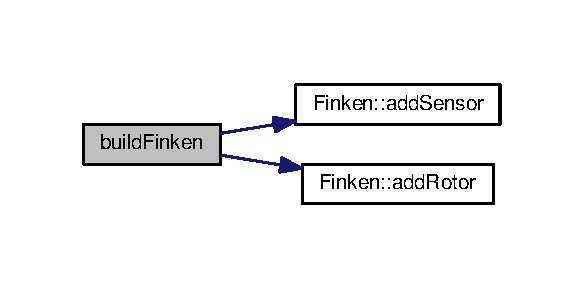
\includegraphics[width=280pt]{finken_8cpp_ab8920c514423348469521fe0063534c4_cgraph}
\end{center}
\end{figure}




Here is the caller graph for this function\+:\nopagebreak
\begin{figure}[H]
\begin{center}
\leavevmode
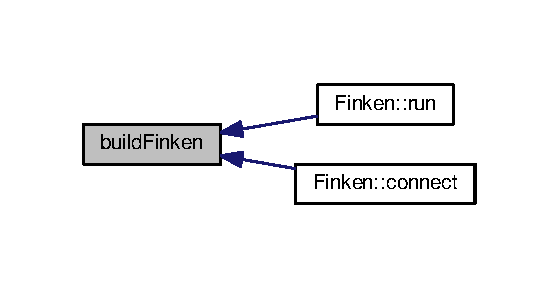
\includegraphics[width=268pt]{finken_8cpp_ab8920c514423348469521fe0063534c4_icgraph}
\end{center}
\end{figure}


\index{finken.\+cpp@{finken.\+cpp}!thrust\+From\+Throttle@{thrust\+From\+Throttle}}
\index{thrust\+From\+Throttle@{thrust\+From\+Throttle}!finken.\+cpp@{finken.\+cpp}}
\subsubsection[{\texorpdfstring{thrust\+From\+Throttle(double throttle)}{thrustFromThrottle(double throttle)}}]{\setlength{\rightskip}{0pt plus 5cm}double thrust\+From\+Throttle (
\begin{DoxyParamCaption}
\item[{double}]{throttle}
\end{DoxyParamCaption}
)}\hypertarget{finken_8cpp_a4e838d73ad5e098825ef4c227f6369b6}{}\label{finken_8cpp_a4e838d73ad5e098825ef4c227f6369b6}


Calculates thrust forces (Newton) from the rotor commands. 

\begin{DoxySeeAlso}{See also}
\hyperlink{classFinken_aa4fe546d88b52ff92990bd67ced70567}{Finken\+::commands} 
\end{DoxySeeAlso}


Here is the caller graph for this function\+:\nopagebreak
\begin{figure}[H]
\begin{center}
\leavevmode
\includegraphics[width=335pt]{finken_8cpp_a4e838d73ad5e098825ef4c227f6369b6_icgraph}
\end{center}
\end{figure}




\subsection{Variable Documentation}
\index{finken.\+cpp@{finken.\+cpp}!csvdata@{csvdata}}
\index{csvdata@{csvdata}!finken.\+cpp@{finken.\+cpp}}
\subsubsection[{\texorpdfstring{csvdata}{csvdata}}]{\setlength{\rightskip}{0pt plus 5cm}ofstream csvdata}\hypertarget{finken_8cpp_ae1ba8f68630cd20b37accfa634ead9c3}{}\label{finken_8cpp_ae1ba8f68630cd20b37accfa634ead9c3}
\index{finken.\+cpp@{finken.\+cpp}!cur\+Block@{cur\+Block}}
\index{cur\+Block@{cur\+Block}!finken.\+cpp@{finken.\+cpp}}
\subsubsection[{\texorpdfstring{cur\+Block}{curBlock}}]{\setlength{\rightskip}{0pt plus 5cm}int cur\+Block}\hypertarget{finken_8cpp_aa9ab2d4a5ee27e4d9984e9d0a25b64d9}{}\label{finken_8cpp_aa9ab2d4a5ee27e4d9984e9d0a25b64d9}
\index{finken.\+cpp@{finken.\+cpp}!in\+Packet@{in\+Packet}}
\index{in\+Packet@{in\+Packet}!finken.\+cpp@{finken.\+cpp}}
\subsubsection[{\texorpdfstring{in\+Packet}{inPacket}}]{\setlength{\rightskip}{0pt plus 5cm}paparazzi\+Packet in\+Packet}\hypertarget{finken_8cpp_a542e7c91dce952d4c1abe4387d0ddb12}{}\label{finken_8cpp_a542e7c91dce952d4c1abe4387d0ddb12}
\index{finken.\+cpp@{finken.\+cpp}!nav\+\_\+block@{nav\+\_\+block}}
\index{nav\+\_\+block@{nav\+\_\+block}!finken.\+cpp@{finken.\+cpp}}
\subsubsection[{\texorpdfstring{nav\+\_\+block}{nav_block}}]{\setlength{\rightskip}{0pt plus 5cm}int nav\+\_\+block}\hypertarget{finken_8cpp_a881d79e252d708b80137d533200ed3ca}{}\label{finken_8cpp_a881d79e252d708b80137d533200ed3ca}
\index{finken.\+cpp@{finken.\+cpp}!out\+Packet@{out\+Packet}}
\index{out\+Packet@{out\+Packet}!finken.\+cpp@{finken.\+cpp}}
\subsubsection[{\texorpdfstring{out\+Packet}{outPacket}}]{\setlength{\rightskip}{0pt plus 5cm}vrep\+Packet out\+Packet}\hypertarget{finken_8cpp_a76246e9f84792114d76311a7aaca677b}{}\label{finken_8cpp_a76246e9f84792114d76311a7aaca677b}
\index{finken.\+cpp@{finken.\+cpp}!read\+Sync@{read\+Sync}}
\index{read\+Sync@{read\+Sync}!finken.\+cpp@{finken.\+cpp}}
\subsubsection[{\texorpdfstring{read\+Sync}{readSync}}]{\setlength{\rightskip}{0pt plus 5cm}std\+::timed\+\_\+mutex read\+Sync}\hypertarget{finken_8cpp_ac4e20dfb154981b9dee8ab3b24dd1778}{}\label{finken_8cpp_ac4e20dfb154981b9dee8ab3b24dd1778}
\index{finken.\+cpp@{finken.\+cpp}!send\+Sync@{send\+Sync}}
\index{send\+Sync@{send\+Sync}!finken.\+cpp@{finken.\+cpp}}
\subsubsection[{\texorpdfstring{send\+Sync}{sendSync}}]{\setlength{\rightskip}{0pt plus 5cm}std\+::timed\+\_\+mutex send\+Sync}\hypertarget{finken_8cpp_a2a73f6002f1b82b5ec6dbfd59171dfd7}{}\label{finken_8cpp_a2a73f6002f1b82b5ec6dbfd59171dfd7}
\index{finken.\+cpp@{finken.\+cpp}!throttlevalues@{throttlevalues}}
\index{throttlevalues@{throttlevalues}!finken.\+cpp@{finken.\+cpp}}
\subsubsection[{\texorpdfstring{throttlevalues}{throttlevalues}}]{\setlength{\rightskip}{0pt plus 5cm}std\+::array$<$double,6$>$ throttlevalues = \{0, 0.\+5, 0.\+65, 0.\+75, 0.\+85, 1\}}\hypertarget{finken_8cpp_a6c6484ebb2a49ce506297ca334add2c4}{}\label{finken_8cpp_a6c6484ebb2a49ce506297ca334add2c4}


Throttlevalues for the motors built into the F\+I\+Nken. 

\index{finken.\+cpp@{finken.\+cpp}!thrustvalues@{thrustvalues}}
\index{thrustvalues@{thrustvalues}!finken.\+cpp@{finken.\+cpp}}
\subsubsection[{\texorpdfstring{thrustvalues}{thrustvalues}}]{\setlength{\rightskip}{0pt plus 5cm}std\+::array$<$double,6$>$ thrustvalues = \{0, 0.\+92,1.\+13,1.\+44,1.\+77,2.\+03\}}\hypertarget{finken_8cpp_a6b9ebe9dad3979425b54b2f62bf0017d}{}\label{finken_8cpp_a6b9ebe9dad3979425b54b2f62bf0017d}


Thrust values in Newton coressponding to the trottle values. 

\index{finken.\+cpp@{finken.\+cpp}!vrep\+Home@{vrep\+Home}}
\index{vrep\+Home@{vrep\+Home}!finken.\+cpp@{finken.\+cpp}}
\subsubsection[{\texorpdfstring{vrep\+Home}{vrepHome}}]{\setlength{\rightskip}{0pt plus 5cm}std\+::string vrep\+Home =std\+::getenv(\char`\"{}V\+R\+E\+P\+\_\+\+H\+O\+ME\char`\"{})}\hypertarget{finken_8cpp_ad8e794da472697af916fedd286d28e33}{}\label{finken_8cpp_ad8e794da472697af916fedd286d28e33}

\hypertarget{finken_8h}{}\section{finken.\+h File Reference}
\label{finken_8h}\index{finken.\+h@{finken.\+h}}


header for the finken implementation  


{\ttfamily \#include $<$memory$>$}\\*
{\ttfamily \#include $<$cstdlib$>$}\\*
{\ttfamily \#include $<$iostream$>$}\\*
{\ttfamily \#include $<$thread$>$}\\*
{\ttfamily \#include $<$utility$>$}\\*
{\ttfamily \#include $<$boost/asio.\+hpp$>$}\\*
{\ttfamily \#include $<$condition\+\_\+variable$>$}\\*
{\ttfamily \#include $<$chrono$>$}\\*
{\ttfamily \#include $<$atomic$>$}\\*
{\ttfamily \#include $<$boost/filesystem.\+hpp$>$}\\*
{\ttfamily \#include $<$boost/filesystem/fstream.\+hpp$>$}\\*
{\ttfamily \#include $<$boost/archive/binary\+\_\+oarchive.\+hpp$>$}\\*
{\ttfamily \#include $<$boost/archive/binary\+\_\+iarchive.\+hpp$>$}\\*
{\ttfamily \#include $<$mutex$>$}\\*
{\ttfamily \#include $<$vector$>$}\\*
{\ttfamily \#include $<$v\+\_\+rep\+Lib.\+h$>$}\\*
{\ttfamily \#include \char`\"{}data\+Packet.\+h\char`\"{}}\\*
{\ttfamily \#include \char`\"{}sensor.\+h\char`\"{}}\\*
{\ttfamily \#include \char`\"{}sonar.\+h\char`\"{}}\\*
{\ttfamily \#include \char`\"{}heightsensor.\+h\char`\"{}}\\*
{\ttfamily \#include \char`\"{}rotor.\+h\char`\"{}}\\*
{\ttfamily \#include \char`\"{}positionsensor.\+h\char`\"{}}\\*
{\ttfamily \#include $<$Eigen/\+Dense$>$}\\*
Include dependency graph for finken.\+h\+:\nopagebreak
\begin{figure}[H]
\begin{center}
\leavevmode
\includegraphics[width=350pt]{finken_8h__incl}
\end{center}
\end{figure}
This graph shows which files directly or indirectly include this file\+:\nopagebreak
\begin{figure}[H]
\begin{center}
\leavevmode
\includegraphics[width=338pt]{finken_8h__dep__incl}
\end{center}
\end{figure}
\subsection*{Classes}
\begin{DoxyCompactItemize}
\item 
class \hyperlink{classLogLine}{Log\+Line}
\begin{DoxyCompactList}\small\item\em Class for annotating log with time points. \end{DoxyCompactList}\item 
class \hyperlink{classVrepLog}{Vrep\+Log}
\begin{DoxyCompactList}\small\item\em Class for creating a log file. \end{DoxyCompactList}\item 
class \hyperlink{classFinken}{Finken}
\begin{DoxyCompactList}\small\item\em \hyperlink{classFinken}{Finken} class for handling any data exchanges between a F\+I\+Nken and Paparazzi. \end{DoxyCompactList}\end{DoxyCompactItemize}
\subsection*{Typedefs}
\begin{DoxyCompactItemize}
\item 
using \hyperlink{finken_8h_accf829b29dcee7a09273bd9101f04e89}{Clock} = std\+::chrono\+::high\+\_\+resolution\+\_\+clock
\end{DoxyCompactItemize}
\subsection*{Functions}
\begin{DoxyCompactItemize}
\item 
void \hyperlink{finken_8h_ab8920c514423348469521fe0063534c4}{build\+Finken} (\hyperlink{classFinken}{Finken} \&finken)
\begin{DoxyCompactList}\small\item\em Constructs a complete F\+I\+Nken from an empty F\+I\+Nken object using its handle. \end{DoxyCompactList}\item 
double \hyperlink{finken_8h_a4e838d73ad5e098825ef4c227f6369b6}{thrust\+From\+Throttle} (double throttle)
\begin{DoxyCompactList}\small\item\em Calculates thrust forces (Newton) from the rotor commands. \end{DoxyCompactList}\end{DoxyCompactItemize}
\subsection*{Variables}
\begin{DoxyCompactItemize}
\item 
std\+::timed\+\_\+mutex \hyperlink{finken_8h_a2a73f6002f1b82b5ec6dbfd59171dfd7}{send\+Sync}
\item 
std\+::timed\+\_\+mutex \hyperlink{finken_8h_ac4e20dfb154981b9dee8ab3b24dd1778}{read\+Sync}
\item 
\hyperlink{classVrepLog}{Vrep\+Log} \hyperlink{finken_8h_a89deba42952826c303251a9d4d45afda}{vrep\+Log}
\end{DoxyCompactItemize}


\subsection{Detailed Description}
header for the finken implementation 



\subsection{Typedef Documentation}
\index{finken.\+h@{finken.\+h}!Clock@{Clock}}
\index{Clock@{Clock}!finken.\+h@{finken.\+h}}
\subsubsection[{\texorpdfstring{Clock}{Clock}}]{\setlength{\rightskip}{0pt plus 5cm}using {\bf Clock} =  std\+::chrono\+::high\+\_\+resolution\+\_\+clock}\hypertarget{finken_8h_accf829b29dcee7a09273bd9101f04e89}{}\label{finken_8h_accf829b29dcee7a09273bd9101f04e89}


\subsection{Function Documentation}
\index{finken.\+h@{finken.\+h}!build\+Finken@{build\+Finken}}
\index{build\+Finken@{build\+Finken}!finken.\+h@{finken.\+h}}
\subsubsection[{\texorpdfstring{build\+Finken(\+Finken \&finken)}{buildFinken(Finken &finken)}}]{\setlength{\rightskip}{0pt plus 5cm}void build\+Finken (
\begin{DoxyParamCaption}
\item[{{\bf Finken} \&}]{finken}
\end{DoxyParamCaption}
)}\hypertarget{finken_8h_ab8920c514423348469521fe0063534c4}{}\label{finken_8h_ab8920c514423348469521fe0063534c4}


Constructs a complete F\+I\+Nken from an empty F\+I\+Nken object using its handle. 

Takes a unique\+\_\+ptr to a \hyperlink{classFinken}{Finken} and adds the correct handles for the sensors \& rotors from the V-\/\+R\+EP object tree. 
\begin{DoxyParams}{Parameters}
{\em finken} & the F\+I\+Nken object to be populated. \\
\hline
\end{DoxyParams}


Here is the call graph for this function\+:\nopagebreak
\begin{figure}[H]
\begin{center}
\leavevmode
\includegraphics[width=280pt]{finken_8h_ab8920c514423348469521fe0063534c4_cgraph}
\end{center}
\end{figure}




Here is the caller graph for this function\+:\nopagebreak
\begin{figure}[H]
\begin{center}
\leavevmode
\includegraphics[width=268pt]{finken_8h_ab8920c514423348469521fe0063534c4_icgraph}
\end{center}
\end{figure}


\index{finken.\+h@{finken.\+h}!thrust\+From\+Throttle@{thrust\+From\+Throttle}}
\index{thrust\+From\+Throttle@{thrust\+From\+Throttle}!finken.\+h@{finken.\+h}}
\subsubsection[{\texorpdfstring{thrust\+From\+Throttle(double throttle)}{thrustFromThrottle(double throttle)}}]{\setlength{\rightskip}{0pt plus 5cm}double thrust\+From\+Throttle (
\begin{DoxyParamCaption}
\item[{double}]{throttle}
\end{DoxyParamCaption}
)}\hypertarget{finken_8h_a4e838d73ad5e098825ef4c227f6369b6}{}\label{finken_8h_a4e838d73ad5e098825ef4c227f6369b6}


Calculates thrust forces (Newton) from the rotor commands. 

\begin{DoxySeeAlso}{See also}
\hyperlink{classFinken_aa4fe546d88b52ff92990bd67ced70567}{Finken\+::commands} 
\end{DoxySeeAlso}


Here is the caller graph for this function\+:\nopagebreak
\begin{figure}[H]
\begin{center}
\leavevmode
\includegraphics[width=335pt]{finken_8h_a4e838d73ad5e098825ef4c227f6369b6_icgraph}
\end{center}
\end{figure}




\subsection{Variable Documentation}
\index{finken.\+h@{finken.\+h}!read\+Sync@{read\+Sync}}
\index{read\+Sync@{read\+Sync}!finken.\+h@{finken.\+h}}
\subsubsection[{\texorpdfstring{read\+Sync}{readSync}}]{\setlength{\rightskip}{0pt plus 5cm}std\+::timed\+\_\+mutex read\+Sync}\hypertarget{finken_8h_ac4e20dfb154981b9dee8ab3b24dd1778}{}\label{finken_8h_ac4e20dfb154981b9dee8ab3b24dd1778}
\index{finken.\+h@{finken.\+h}!send\+Sync@{send\+Sync}}
\index{send\+Sync@{send\+Sync}!finken.\+h@{finken.\+h}}
\subsubsection[{\texorpdfstring{send\+Sync}{sendSync}}]{\setlength{\rightskip}{0pt plus 5cm}std\+::timed\+\_\+mutex send\+Sync}\hypertarget{finken_8h_a2a73f6002f1b82b5ec6dbfd59171dfd7}{}\label{finken_8h_a2a73f6002f1b82b5ec6dbfd59171dfd7}
\index{finken.\+h@{finken.\+h}!vrep\+Log@{vrep\+Log}}
\index{vrep\+Log@{vrep\+Log}!finken.\+h@{finken.\+h}}
\subsubsection[{\texorpdfstring{vrep\+Log}{vrepLog}}]{\setlength{\rightskip}{0pt plus 5cm}{\bf Vrep\+Log} vrep\+Log}\hypertarget{finken_8h_a89deba42952826c303251a9d4d45afda}{}\label{finken_8h_a89deba42952826c303251a9d4d45afda}

\hypertarget{finkenplugin_8cpp}{}\section{finkenplugin.\+cpp File Reference}
\label{finkenplugin_8cpp}\index{finkenplugin.\+cpp@{finkenplugin.\+cpp}}
{\ttfamily \#include $<$vrepplugin.\+h$>$}\\*
{\ttfamily \#include $<$log.\+h$>$}\\*
{\ttfamily \#include \char`\"{}finken.\+h\char`\"{}}\\*
{\ttfamily \#include \char`\"{}v\+\_\+rep\+Lib.\+h\char`\"{}}\\*
{\ttfamily \#include $<$unistd.\+h$>$}\\*
{\ttfamily \#include $<$iostream$>$}\\*
{\ttfamily \#include $<$positionsensor.\+h$>$}\\*
{\ttfamily \#include $<$cstring$>$}\\*
{\ttfamily \#include $<$cstdlib$>$}\\*
{\ttfamily \#include $<$thread$>$}\\*
{\ttfamily \#include $<$memory$>$}\\*
{\ttfamily \#include $<$utility$>$}\\*
{\ttfamily \#include $<$boost/asio.\+hpp$>$}\\*
{\ttfamily \#include $<$boost/bind.\+hpp$>$}\\*
{\ttfamily \#include $<$boost/thread.\+hpp$>$}\\*
{\ttfamily \#include $<$boost/archive/text\+\_\+oarchive.\+hpp$>$}\\*
{\ttfamily \#include $<$boost/archive/text\+\_\+iarchive.\+hpp$>$}\\*
{\ttfamily \#include $<$condition\+\_\+variable$>$}\\*
{\ttfamily \#include $<$chrono$>$}\\*
{\ttfamily \#include $<$Eigen/\+Dense$>$}\\*
Include dependency graph for finkenplugin.\+cpp\+:
% FIG 0
\subsection*{Classes}
\begin{DoxyCompactItemize}
\item 
class \hyperlink{classAsync__Server}{Async\+\_\+\+Server}
\begin{DoxyCompactList}\small\item\em Asynchronous (boost\+::\+Asio) Server class to accept new paparazzi connections and pair them with a vrep copter. \end{DoxyCompactList}\item 
class \hyperlink{classFinkenPlugin}{Finken\+Plugin}
\begin{DoxyCompactList}\small\item\em implementation of the baseline functionality for the plugin and the communication, including the server class \end{DoxyCompactList}\end{DoxyCompactItemize}
\subsection*{Typedefs}
\begin{DoxyCompactItemize}
\item 
using {\bfseries Clock} = std\+::chrono\+::high\+\_\+resolution\+\_\+clock\hypertarget{finkenplugin_8cpp_accf829b29dcee7a09273bd9101f04e89}{}\label{finkenplugin_8cpp_accf829b29dcee7a09273bd9101f04e89}

\end{DoxyCompactItemize}
\subsection*{Variables}
\begin{DoxyCompactItemize}
\item 
bool {\bfseries server\+Loaded} = false\hypertarget{finkenplugin_8cpp_a648687a718c8aefc5299af32cfc58c3a}{}\label{finkenplugin_8cpp_a648687a718c8aefc5299af32cfc58c3a}

\item 
bool {\bfseries connection\+Established} = false\hypertarget{finkenplugin_8cpp_aa5ac184beede4085dca63f64e6406ead}{}\label{finkenplugin_8cpp_aa5ac184beede4085dca63f64e6406ead}

\item 
float {\bfseries execution\+\_\+step\+\_\+size}\hypertarget{finkenplugin_8cpp_a88a0adfc978c2e320204dcfd93415429}{}\label{finkenplugin_8cpp_a88a0adfc978c2e320204dcfd93415429}

\item 
std\+::vector$<$ std\+::unique\+\_\+ptr$<$ \hyperlink{classFinken}{Finken} $>$ $>$ \hyperlink{finkenplugin_8cpp_afb23cb5abeeb0dfc99c4382ba7d4eebd}{sim\+Finken}
\item 
std\+::unique\+\_\+ptr$<$ tcp\+::iostream $>$ {\bfseries s\+Ptr}\hypertarget{finkenplugin_8cpp_ac7413237502a08f3a3cb45e20174e71d}{}\label{finkenplugin_8cpp_ac7413237502a08f3a3cb45e20174e71d}

\item 
\hyperlink{classVrepLog}{Vrep\+Log} {\bfseries vrep\+Log}\hypertarget{finkenplugin_8cpp_a89deba42952826c303251a9d4d45afda}{}\label{finkenplugin_8cpp_a89deba42952826c303251a9d4d45afda}

\item 
paparazzi\+Packet {\bfseries first\+Packet}\hypertarget{finkenplugin_8cpp_a8e45d67c7cca60311773160c7ea56eee}{}\label{finkenplugin_8cpp_a8e45d67c7cca60311773160c7ea56eee}

\item 
\hyperlink{classFinkenPlugin}{Finken\+Plugin} {\bfseries plugin}\hypertarget{finkenplugin_8cpp_a4152403e715dc2efffb6d1393f654c17}{}\label{finkenplugin_8cpp_a4152403e715dc2efffb6d1393f654c17}

\end{DoxyCompactItemize}


\subsection{Variable Documentation}
\index{finkenplugin.\+cpp@{finkenplugin.\+cpp}!sim\+Finken@{sim\+Finken}}
\index{sim\+Finken@{sim\+Finken}!finkenplugin.\+cpp@{finkenplugin.\+cpp}}
\subsubsection[{\texorpdfstring{sim\+Finken}{simFinken}}]{\setlength{\rightskip}{0pt plus 5cm}std\+::vector$<$std\+::unique\+\_\+ptr$<${\bf Finken}$>$ $>$ sim\+Finken}\hypertarget{finkenplugin_8cpp_afb23cb5abeeb0dfc99c4382ba7d4eebd}{}\label{finkenplugin_8cpp_afb23cb5abeeb0dfc99c4382ba7d4eebd}
\label{skeleton_8cpp_simFinken}%
\hypertarget{skeleton_8cpp_simFinken}{}%
Vector for all available (e.\+g. present in the plugin) copters 
\hypertarget{heightsensor_8cpp}{}\section{heightsensor.\+cpp File Reference}
\label{heightsensor_8cpp}\index{heightsensor.\+cpp@{heightsensor.\+cpp}}
{\ttfamily \#include \char`\"{}heightsensor.\+h\char`\"{}}\\*
{\ttfamily \#include \char`\"{}v\+\_\+rep\+Lib.\+h\char`\"{}}\\*
{\ttfamily \#include $<$iostream$>$}\\*
Include dependency graph for heightsensor.\+cpp\+:\nopagebreak
\begin{figure}[H]
\begin{center}
\leavevmode
\includegraphics[width=312pt]{heightsensor_8cpp__incl}
\end{center}
\end{figure}

\hypertarget{heightsensor_8h}{}\section{heightsensor.\+h File Reference}
\label{heightsensor_8h}\index{heightsensor.\+h@{heightsensor.\+h}}
{\ttfamily \#include \char`\"{}sensor.\+h\char`\"{}}\\*
Include dependency graph for heightsensor.\+h\+:\nopagebreak
\begin{figure}[H]
\begin{center}
\leavevmode
\includegraphics[width=160pt]{heightsensor_8h__incl}
\end{center}
\end{figure}
This graph shows which files directly or indirectly include this file\+:\nopagebreak
\begin{figure}[H]
\begin{center}
\leavevmode
\includegraphics[width=339pt]{heightsensor_8h__dep__incl}
\end{center}
\end{figure}
\subsection*{Classes}
\begin{DoxyCompactItemize}
\item 
class \hyperlink{classHeightSensor}{Height\+Sensor}
\begin{DoxyCompactList}\small\item\em Class implementing a heightsensor. \end{DoxyCompactList}\end{DoxyCompactItemize}

\hypertarget{log_8cpp}{}\section{log.\+cpp File Reference}
\label{log_8cpp}\index{log.\+cpp@{log.\+cpp}}
{\ttfamily \#include $<$log.\+h$>$}\\*
{\ttfamily \#include $<$iostream$>$}\\*
Include dependency graph for log.\+cpp\+:\nopagebreak
\begin{figure}[H]
\begin{center}
\leavevmode
\includegraphics[width=229pt]{log_8cpp__incl}
\end{center}
\end{figure}

\hypertarget{log_8h}{}\section{log.\+h File Reference}
\label{log_8h}\index{log.\+h@{log.\+h}}
{\ttfamily \#include $<$ostream$>$}\\*
{\ttfamily \#include $<$string$>$}\\*
Include dependency graph for log.\+h\+:\nopagebreak
\begin{figure}[H]
\begin{center}
\leavevmode
\includegraphics[width=192pt]{log_8h__incl}
\end{center}
\end{figure}
This graph shows which files directly or indirectly include this file\+:\nopagebreak
\begin{figure}[H]
\begin{center}
\leavevmode
\includegraphics[width=234pt]{log_8h__dep__incl}
\end{center}
\end{figure}
\subsection*{Classes}
\begin{DoxyCompactItemize}
\item 
class \hyperlink{classLog}{Log}
\begin{DoxyCompactList}\small\item\em Baisc logging class. \end{DoxyCompactList}\end{DoxyCompactItemize}

\hypertarget{mainpage_8txt}{}\section{mainpage.\+txt File Reference}
\label{mainpage_8txt}\index{mainpage.\+txt@{mainpage.\+txt}}

\hypertarget{positionsensor_8cpp}{}\section{positionsensor.\+cpp File Reference}
\label{positionsensor_8cpp}\index{positionsensor.\+cpp@{positionsensor.\+cpp}}
{\ttfamily \#include \char`\"{}positionsensor.\+h\char`\"{}}\\*
{\ttfamily \#include \char`\"{}v\+\_\+rep\+Lib.\+h\char`\"{}}\\*
{\ttfamily \#include $<$iostream$>$}\\*
{\ttfamily \#include $<$vector$>$}\\*
Include dependency graph for positionsensor.\+cpp\+:
% FIG 0

\hypertarget{positionsensor_8h}{}\section{positionsensor.\+h File Reference}
\label{positionsensor_8h}\index{positionsensor.\+h@{positionsensor.\+h}}
{\ttfamily \#include \char`\"{}sensor.\+h\char`\"{}}\\*
Include dependency graph for positionsensor.\+h\+:\nopagebreak
\begin{figure}[H]
\begin{center}
\leavevmode
\includegraphics[width=168pt]{positionsensor_8h__incl}
\end{center}
\end{figure}
This graph shows which files directly or indirectly include this file\+:\nopagebreak
\begin{figure}[H]
\begin{center}
\leavevmode
\includegraphics[width=350pt]{positionsensor_8h__dep__incl}
\end{center}
\end{figure}
\subsection*{Classes}
\begin{DoxyCompactItemize}
\item 
class \hyperlink{classPositionSensor}{Position\+Sensor}
\begin{DoxyCompactList}\small\item\em wrapper to disguise vrep A\+PI calls as a position sensor \end{DoxyCompactList}\end{DoxyCompactItemize}

\hypertarget{rotor_8cpp}{}\section{rotor.\+cpp File Reference}
\label{rotor_8cpp}\index{rotor.\+cpp@{rotor.\+cpp}}
{\ttfamily \#include \char`\"{}rotor.\+h\char`\"{}}\\*
{\ttfamily \#include \char`\"{}v\+\_\+rep\+Lib.\+h\char`\"{}}\\*
Include dependency graph for rotor.\+cpp\+:
% FIG 0

\hypertarget{rotor_8h}{}\section{rotor.\+h File Reference}
\label{rotor_8h}\index{rotor.\+h@{rotor.\+h}}
{\ttfamily \#include $<$vector$>$}\\*
Include dependency graph for rotor.\+h\+:\nopagebreak
\begin{figure}[H]
\begin{center}
\leavevmode
\includegraphics[width=124pt]{rotor_8h__incl}
\end{center}
\end{figure}
This graph shows which files directly or indirectly include this file\+:\nopagebreak
\begin{figure}[H]
\begin{center}
\leavevmode
\includegraphics[width=338pt]{rotor_8h__dep__incl}
\end{center}
\end{figure}
\subsection*{Classes}
\begin{DoxyCompactItemize}
\item 
class \hyperlink{classRotor}{Rotor}
\begin{DoxyCompactList}\small\item\em Implementation of a force sensor as a rotor. \end{DoxyCompactList}\end{DoxyCompactItemize}

\hypertarget{sensor_8cpp}{}\section{sensor.\+cpp File Reference}
\label{sensor_8cpp}\index{sensor.\+cpp@{sensor.\+cpp}}
{\ttfamily \#include \char`\"{}sensor.\+h\char`\"{}}\\*
{\ttfamily \#include $<$iostream$>$}\\*
Include dependency graph for sensor.\+cpp\+:\nopagebreak
\begin{figure}[H]
\begin{center}
\leavevmode
\includegraphics[width=206pt]{sensor_8cpp__incl}
\end{center}
\end{figure}

\hypertarget{sensor_8h}{}\section{sensor.\+h File Reference}
\label{sensor_8h}\index{sensor.\+h@{sensor.\+h}}
{\ttfamily \#include $<$vector$>$}\\*
Include dependency graph for sensor.\+h\+:\nopagebreak
\begin{figure}[H]
\begin{center}
\leavevmode
\includegraphics[width=134pt]{sensor_8h__incl}
\end{center}
\end{figure}
This graph shows which files directly or indirectly include this file\+:\nopagebreak
\begin{figure}[H]
\begin{center}
\leavevmode
\includegraphics[width=350pt]{sensor_8h__dep__incl}
\end{center}
\end{figure}
\subsection*{Classes}
\begin{DoxyCompactItemize}
\item 
class \hyperlink{classSensor}{Sensor}
\begin{DoxyCompactList}\small\item\em base \hyperlink{classSensor}{Sensor} class, all sensors should inherit from this \end{DoxyCompactList}\end{DoxyCompactItemize}

\hypertarget{skeleton_8cpp}{}\section{skeleton.\+cpp File Reference}
\label{skeleton_8cpp}\index{skeleton.\+cpp@{skeleton.\+cpp}}


provides the basic functionality for communication with the running vrep Simulation"  


{\ttfamily \#include $<$vrepplugin.\+h$>$}\\*
{\ttfamily \#include $<$v\+\_\+rep\+Lib.\+h$>$}\\*
{\ttfamily \#include $<$script\+Function\+Data.\+h$>$}\\*
{\ttfamily \#include $<$boost/filesystem.\+hpp$>$}\\*
{\ttfamily \#include $<$iostream$>$}\\*
{\ttfamily \#include $<$finken.\+h$>$}\\*
Include dependency graph for skeleton.\+cpp\+:\nopagebreak
\begin{figure}[H]
\begin{center}
\leavevmode
\includegraphics[width=350pt]{skeleton_8cpp__incl}
\end{center}
\end{figure}
\subsection*{Macros}
\begin{DoxyCompactItemize}
\item 
\#define \hyperlink{skeleton_8cpp_ad74f6239255ddea51d1921e596831913}{L\+U\+A\+\_\+\+R\+E\+G\+I\+S\+T\+E\+R\+\_\+\+C\+O\+M\+M\+A\+ND}~\char`\"{}sim\+Ext\+Paparazzi\+\_\+register\char`\"{}
\end{DoxyCompactItemize}
\subsection*{Functions}
\begin{DoxyCompactItemize}
\item 
void \hyperlink{skeleton_8cpp_a8b710f83dc7306a1f10184e7c50cc921}{L\+U\+A\+\_\+\+R\+E\+G\+I\+S\+T\+E\+R\+\_\+\+C\+A\+L\+L\+B\+A\+CK} (S\+Script\+Call\+Back $\ast$cb)
\begin{DoxyCompactList}\small\item\em Function to register any F\+I\+Nken present in the vrep scene with the plugin. \end{DoxyCompactList}\end{DoxyCompactItemize}
\begin{Indent}{\bf vrep entry points}\par
{\em Required entry points for vrep plugin functions.

Vrep Doc\+: \href{http://www.coppeliarobotics.com/helpFiles/en/plugins.htm}{\tt http\+://www.\+coppeliarobotics.\+com/help\+Files/en/plugins.\+htm} }\begin{DoxyCompactItemize}
\item 
unsigned char \hyperlink{skeleton_8cpp_af17a7ec1007534f93373d28449776791}{v\+\_\+rep\+Start} (void $\ast$reserved\+Pointer, int reserved\+Int)
\item 
void \hyperlink{skeleton_8cpp_af26d39e198d72e89ff60386e9fd18516}{v\+\_\+rep\+End} ()
\item 
void $\ast$ \hyperlink{skeleton_8cpp_a2edf50a75bd96c6ed31c1da66828af6e}{v\+\_\+rep\+Message} (int message, int $\ast$auxiliary\+Data, void $\ast$custom\+Data, int $\ast$reply\+Data)
\end{DoxyCompactItemize}
\end{Indent}
\subsection*{Variables}
\begin{DoxyCompactItemize}
\item 
L\+I\+B\+R\+A\+RY \hyperlink{skeleton_8cpp_a547ddb2140854533efea77ef084548f2}{vrep\+Lib}
\item 
const char $\ast$ \hyperlink{skeleton_8cpp_a089f78fbca1c19d7d6fcd2a3669f79d2}{lib\+Name} =\char`\"{}libv\+\_\+rep.\+so\char`\"{}
\item 
std\+::vector$<$ std\+::unique\+\_\+ptr$<$ \hyperlink{classFinken}{Finken} $>$ $>$ \hyperlink{skeleton_8cpp_afb23cb5abeeb0dfc99c4382ba7d4eebd}{sim\+Finken}
\item 
const int \hyperlink{skeleton_8cpp_a148b31424ba0940f7b48221aedd08fad}{in\+Args\+\_\+\+R\+E\+G\+I\+S\+T\+ER} \mbox{[}$\,$\mbox{]}
\end{DoxyCompactItemize}


\subsection{Detailed Description}
provides the basic functionality for communication with the running vrep Simulation" 



\subsection{Macro Definition Documentation}
\index{skeleton.\+cpp@{skeleton.\+cpp}!L\+U\+A\+\_\+\+R\+E\+G\+I\+S\+T\+E\+R\+\_\+\+C\+O\+M\+M\+A\+ND@{L\+U\+A\+\_\+\+R\+E\+G\+I\+S\+T\+E\+R\+\_\+\+C\+O\+M\+M\+A\+ND}}
\index{L\+U\+A\+\_\+\+R\+E\+G\+I\+S\+T\+E\+R\+\_\+\+C\+O\+M\+M\+A\+ND@{L\+U\+A\+\_\+\+R\+E\+G\+I\+S\+T\+E\+R\+\_\+\+C\+O\+M\+M\+A\+ND}!skeleton.\+cpp@{skeleton.\+cpp}}
\subsubsection[{\texorpdfstring{L\+U\+A\+\_\+\+R\+E\+G\+I\+S\+T\+E\+R\+\_\+\+C\+O\+M\+M\+A\+ND}{LUA_REGISTER_COMMAND}}]{\setlength{\rightskip}{0pt plus 5cm}\#define L\+U\+A\+\_\+\+R\+E\+G\+I\+S\+T\+E\+R\+\_\+\+C\+O\+M\+M\+A\+ND~\char`\"{}sim\+Ext\+Paparazzi\+\_\+register\char`\"{}}\hypertarget{skeleton_8cpp_ad74f6239255ddea51d1921e596831913}{}\label{skeleton_8cpp_ad74f6239255ddea51d1921e596831913}


\subsection{Function Documentation}
\index{skeleton.\+cpp@{skeleton.\+cpp}!L\+U\+A\+\_\+\+R\+E\+G\+I\+S\+T\+E\+R\+\_\+\+C\+A\+L\+L\+B\+A\+CK@{L\+U\+A\+\_\+\+R\+E\+G\+I\+S\+T\+E\+R\+\_\+\+C\+A\+L\+L\+B\+A\+CK}}
\index{L\+U\+A\+\_\+\+R\+E\+G\+I\+S\+T\+E\+R\+\_\+\+C\+A\+L\+L\+B\+A\+CK@{L\+U\+A\+\_\+\+R\+E\+G\+I\+S\+T\+E\+R\+\_\+\+C\+A\+L\+L\+B\+A\+CK}!skeleton.\+cpp@{skeleton.\+cpp}}
\subsubsection[{\texorpdfstring{L\+U\+A\+\_\+\+R\+E\+G\+I\+S\+T\+E\+R\+\_\+\+C\+A\+L\+L\+B\+A\+C\+K(\+S\+Script\+Call\+Back $\ast$cb)}{LUA_REGISTER_CALLBACK(SScriptCallBack *cb)}}]{\setlength{\rightskip}{0pt plus 5cm}void L\+U\+A\+\_\+\+R\+E\+G\+I\+S\+T\+E\+R\+\_\+\+C\+A\+L\+L\+B\+A\+CK (
\begin{DoxyParamCaption}
\item[{S\+Script\+Call\+Back $\ast$}]{cb}
\end{DoxyParamCaption}
)}\hypertarget{skeleton_8cpp_a8b710f83dc7306a1f10184e7c50cc921}{}\label{skeleton_8cpp_a8b710f83dc7306a1f10184e7c50cc921}


Function to register any F\+I\+Nken present in the vrep scene with the plugin. 

Every copter needs to call this in its child script to be accesible by the plugin. Stores the handle, aricraft\+ID, rotor and sonar counts in \hyperlink{skeleton_8cpp_simFinken}{sim\+Finken} 

Here is the caller graph for this function\+:\nopagebreak
\begin{figure}[H]
\begin{center}
\leavevmode
\includegraphics[width=329pt]{skeleton_8cpp_a8b710f83dc7306a1f10184e7c50cc921_icgraph}
\end{center}
\end{figure}


\index{skeleton.\+cpp@{skeleton.\+cpp}!v\+\_\+rep\+End@{v\+\_\+rep\+End}}
\index{v\+\_\+rep\+End@{v\+\_\+rep\+End}!skeleton.\+cpp@{skeleton.\+cpp}}
\subsubsection[{\texorpdfstring{v\+\_\+rep\+End()}{v_repEnd()}}]{\setlength{\rightskip}{0pt plus 5cm}void v\+\_\+rep\+End (
\begin{DoxyParamCaption}
{}
\end{DoxyParamCaption}
)}\hypertarget{skeleton_8cpp_af26d39e198d72e89ff60386e9fd18516}{}\label{skeleton_8cpp_af26d39e198d72e89ff60386e9fd18516}


Here is the call graph for this function\+:\nopagebreak
\begin{figure}[H]
\begin{center}
\leavevmode
\includegraphics[width=302pt]{skeleton_8cpp_af26d39e198d72e89ff60386e9fd18516_cgraph}
\end{center}
\end{figure}


\index{skeleton.\+cpp@{skeleton.\+cpp}!v\+\_\+rep\+Message@{v\+\_\+rep\+Message}}
\index{v\+\_\+rep\+Message@{v\+\_\+rep\+Message}!skeleton.\+cpp@{skeleton.\+cpp}}
\subsubsection[{\texorpdfstring{v\+\_\+rep\+Message(int message, int $\ast$auxiliary\+Data, void $\ast$custom\+Data, int $\ast$reply\+Data)}{v_repMessage(int message, int *auxiliaryData, void *customData, int *replyData)}}]{\setlength{\rightskip}{0pt plus 5cm}void$\ast$ v\+\_\+rep\+Message (
\begin{DoxyParamCaption}
\item[{int}]{message, }
\item[{int $\ast$}]{auxiliary\+Data, }
\item[{void $\ast$}]{custom\+Data, }
\item[{int $\ast$}]{reply\+Data}
\end{DoxyParamCaption}
)}\hypertarget{skeleton_8cpp_a2edf50a75bd96c6ed31c1da66828af6e}{}\label{skeleton_8cpp_a2edf50a75bd96c6ed31c1da66828af6e}


Here is the call graph for this function\+:\nopagebreak
\begin{figure}[H]
\begin{center}
\leavevmode
\includegraphics[height=550pt]{skeleton_8cpp_a2edf50a75bd96c6ed31c1da66828af6e_cgraph}
\end{center}
\end{figure}


\index{skeleton.\+cpp@{skeleton.\+cpp}!v\+\_\+rep\+Start@{v\+\_\+rep\+Start}}
\index{v\+\_\+rep\+Start@{v\+\_\+rep\+Start}!skeleton.\+cpp@{skeleton.\+cpp}}
\subsubsection[{\texorpdfstring{v\+\_\+rep\+Start(void $\ast$reserved\+Pointer, int reserved\+Int)}{v_repStart(void *reservedPointer, int reservedInt)}}]{\setlength{\rightskip}{0pt plus 5cm}unsigned char v\+\_\+rep\+Start (
\begin{DoxyParamCaption}
\item[{void $\ast$}]{reserved\+Pointer, }
\item[{int}]{reserved\+Int}
\end{DoxyParamCaption}
)}\hypertarget{skeleton_8cpp_af17a7ec1007534f93373d28449776791}{}\label{skeleton_8cpp_af17a7ec1007534f93373d28449776791}


Here is the call graph for this function\+:\nopagebreak
\begin{figure}[H]
\begin{center}
\leavevmode
\includegraphics[width=329pt]{skeleton_8cpp_af17a7ec1007534f93373d28449776791_cgraph}
\end{center}
\end{figure}




\subsection{Variable Documentation}
\index{skeleton.\+cpp@{skeleton.\+cpp}!in\+Args\+\_\+\+R\+E\+G\+I\+S\+T\+ER@{in\+Args\+\_\+\+R\+E\+G\+I\+S\+T\+ER}}
\index{in\+Args\+\_\+\+R\+E\+G\+I\+S\+T\+ER@{in\+Args\+\_\+\+R\+E\+G\+I\+S\+T\+ER}!skeleton.\+cpp@{skeleton.\+cpp}}
\subsubsection[{\texorpdfstring{in\+Args\+\_\+\+R\+E\+G\+I\+S\+T\+ER}{inArgs_REGISTER}}]{\setlength{\rightskip}{0pt plus 5cm}const int in\+Args\+\_\+\+R\+E\+G\+I\+S\+T\+ER\mbox{[}$\,$\mbox{]}}\hypertarget{skeleton_8cpp_a148b31424ba0940f7b48221aedd08fad}{}\label{skeleton_8cpp_a148b31424ba0940f7b48221aedd08fad}
{\bfseries Initial value\+:}
\begin{DoxyCode}
=\{
    
    4,
    sim\_script\_arg\_int32,0,
    sim\_script\_arg\_int32,0,
    sim\_script\_arg\_int32,0,
    sim\_script\_arg\_int32,0,

\}
\end{DoxyCode}
\index{skeleton.\+cpp@{skeleton.\+cpp}!lib\+Name@{lib\+Name}}
\index{lib\+Name@{lib\+Name}!skeleton.\+cpp@{skeleton.\+cpp}}
\subsubsection[{\texorpdfstring{lib\+Name}{libName}}]{\setlength{\rightskip}{0pt plus 5cm}const char$\ast$ lib\+Name =\char`\"{}libv\+\_\+rep.\+so\char`\"{}}\hypertarget{skeleton_8cpp_a089f78fbca1c19d7d6fcd2a3669f79d2}{}\label{skeleton_8cpp_a089f78fbca1c19d7d6fcd2a3669f79d2}
\index{skeleton.\+cpp@{skeleton.\+cpp}!sim\+Finken@{sim\+Finken}}
\index{sim\+Finken@{sim\+Finken}!skeleton.\+cpp@{skeleton.\+cpp}}
\subsubsection[{\texorpdfstring{sim\+Finken}{simFinken}}]{\setlength{\rightskip}{0pt plus 5cm}std\+::vector$<$std\+::unique\+\_\+ptr$<${\bf Finken}$>$ $>$ sim\+Finken}\hypertarget{skeleton_8cpp_afb23cb5abeeb0dfc99c4382ba7d4eebd}{}\label{skeleton_8cpp_afb23cb5abeeb0dfc99c4382ba7d4eebd}
\label{skeleton_8cpp_simFinken}%
\hypertarget{skeleton_8cpp_simFinken}{}%
Vector for all available (e.\+g. present in the plugin) copters \index{skeleton.\+cpp@{skeleton.\+cpp}!vrep\+Lib@{vrep\+Lib}}
\index{vrep\+Lib@{vrep\+Lib}!skeleton.\+cpp@{skeleton.\+cpp}}
\subsubsection[{\texorpdfstring{vrep\+Lib}{vrepLib}}]{\setlength{\rightskip}{0pt plus 5cm}L\+I\+B\+R\+A\+RY vrep\+Lib}\hypertarget{skeleton_8cpp_a547ddb2140854533efea77ef084548f2}{}\label{skeleton_8cpp_a547ddb2140854533efea77ef084548f2}

\hypertarget{sonar_8cpp}{}\section{sonar.\+cpp File Reference}
\label{sonar_8cpp}\index{sonar.\+cpp@{sonar.\+cpp}}
{\ttfamily \#include \char`\"{}sonar.\+h\char`\"{}}\\*
{\ttfamily \#include \char`\"{}v\+\_\+rep\+Lib.\+h\char`\"{}}\\*
{\ttfamily \#include $<$iostream$>$}\\*
Include dependency graph for sonar.\+cpp\+:
% FIG 0

\hypertarget{sonar_8h}{}\section{sonar.\+h File Reference}
\label{sonar_8h}\index{sonar.\+h@{sonar.\+h}}
{\ttfamily \#include \char`\"{}sensor.\+h\char`\"{}}\\*
{\ttfamily \#include $<$string$>$}\\*
Include dependency graph for sonar.\+h\+:\nopagebreak
\begin{figure}[H]
\begin{center}
\leavevmode
\includegraphics[width=194pt]{sonar_8h__incl}
\end{center}
\end{figure}
This graph shows which files directly or indirectly include this file\+:\nopagebreak
\begin{figure}[H]
\begin{center}
\leavevmode
\includegraphics[width=338pt]{sonar_8h__dep__incl}
\end{center}
\end{figure}
\subsection*{Classes}
\begin{DoxyCompactItemize}
\item 
class \hyperlink{classSonar}{Sonar}
\begin{DoxyCompactList}\small\item\em implementation of a proximitysensor as sonar \end{DoxyCompactList}\end{DoxyCompactItemize}

\hypertarget{test_8cpp}{}\section{test.\+cpp File Reference}
\label{test_8cpp}\index{test.\+cpp@{test.\+cpp}}
{\ttfamily \#include $<$Eigen/\+Core$>$}\\*
{\ttfamily \#include $<$boost/serialization/serialization.\+hpp$>$}\\*
{\ttfamily \#include $<$boost/serialization/split\+\_\+free.\+hpp$>$}\\*
{\ttfamily \#include $<$boost/archive/text\+\_\+iarchive.\+hpp$>$}\\*
{\ttfamily \#include $<$boost/archive/text\+\_\+oarchive.\+hpp$>$}\\*
{\ttfamily \#include $<$fstream$>$}\\*
{\ttfamily \#include $<$iostream$>$}\\*
Include dependency graph for test.\+cpp\+:\nopagebreak
\begin{figure}[H]
\begin{center}
\leavevmode
\includegraphics[width=350pt]{test_8cpp__incl}
\end{center}
\end{figure}
\subsection*{Namespaces}
\begin{DoxyCompactItemize}
\item 
 \hyperlink{namespaceboost}{boost}
\item 
 \hyperlink{namespaceboost_1_1serialization}{boost\+::serialization}
\end{DoxyCompactItemize}
\subsection*{Typedefs}
\begin{DoxyCompactItemize}
\item 
using \hyperlink{test_8cpp_a645222978e81acfb2523a9bce34aecc0}{Matrix} = Eigen\+::\+Matrix\+Xf
\item 
using \hyperlink{test_8cpp_aca2956bc379bce2ed88ab3c0e1b61d1d}{Vector} = Eigen\+::\+Vector\+Xf
\end{DoxyCompactItemize}
\subsection*{Functions}
\begin{DoxyCompactItemize}
\item 
{\footnotesize template$<$typename T , int rows, int cols, class Archive $>$ }\\void \hyperlink{namespaceboost_1_1serialization_aa7021b16faca824017a33df205f44c01}{boost\+::serialization\+::save} (Archive \&ar, const \+::\hyperlink{test_8cpp_a645222978e81acfb2523a9bce34aecc0}{Eigen\+::\+Matrix}$<$ T, rows, cols $>$ \&m, unsigned int v)
\item 
{\footnotesize template$<$typename T , int R, int C, class Archive $>$ }\\void \hyperlink{namespaceboost_1_1serialization_a76faf89a36520a5181fe7464aec003fe}{boost\+::serialization\+::load} (Archive \&ar,\+::\hyperlink{test_8cpp_a645222978e81acfb2523a9bce34aecc0}{Eigen\+::\+Matrix}$<$ T, R, C $>$ \&m, unsigned int v)
\item 
{\footnotesize template$<$typename T , int rows, int cols, class Archive $>$ }\\void \hyperlink{namespaceboost_1_1serialization_a5839810cadeccc13a50f63a8cae475a5}{boost\+::serialization\+::serialize} (Archive \&ar,\+::\hyperlink{test_8cpp_a645222978e81acfb2523a9bce34aecc0}{Eigen\+::\+Matrix}$<$ T, rows, cols $>$ \&m, unsigned int file\+\_\+version)
\item 
int \hyperlink{test_8cpp_ae66f6b31b5ad750f1fe042a706a4e3d4}{main} ()
\end{DoxyCompactItemize}


\subsection{Typedef Documentation}
\index{test.\+cpp@{test.\+cpp}!Matrix@{Matrix}}
\index{Matrix@{Matrix}!test.\+cpp@{test.\+cpp}}
\subsubsection[{\texorpdfstring{Matrix}{Matrix}}]{\setlength{\rightskip}{0pt plus 5cm}using {\bf Matrix} =  Eigen\+::\+Matrix\+Xf}\hypertarget{test_8cpp_a645222978e81acfb2523a9bce34aecc0}{}\label{test_8cpp_a645222978e81acfb2523a9bce34aecc0}
\index{test.\+cpp@{test.\+cpp}!Vector@{Vector}}
\index{Vector@{Vector}!test.\+cpp@{test.\+cpp}}
\subsubsection[{\texorpdfstring{Vector}{Vector}}]{\setlength{\rightskip}{0pt plus 5cm}using {\bf Vector} =  Eigen\+::\+Vector\+Xf}\hypertarget{test_8cpp_aca2956bc379bce2ed88ab3c0e1b61d1d}{}\label{test_8cpp_aca2956bc379bce2ed88ab3c0e1b61d1d}


\subsection{Function Documentation}
\index{test.\+cpp@{test.\+cpp}!main@{main}}
\index{main@{main}!test.\+cpp@{test.\+cpp}}
\subsubsection[{\texorpdfstring{main()}{main()}}]{\setlength{\rightskip}{0pt plus 5cm}int main (
\begin{DoxyParamCaption}
{}
\end{DoxyParamCaption}
)}\hypertarget{test_8cpp_ae66f6b31b5ad750f1fe042a706a4e3d4}{}\label{test_8cpp_ae66f6b31b5ad750f1fe042a706a4e3d4}

\hypertarget{vrepplugin_8cpp}{}\section{vrepplugin.\+cpp File Reference}
\label{vrepplugin_8cpp}\index{vrepplugin.\+cpp@{vrepplugin.\+cpp}}
{\ttfamily \#include $<$vrepplugin.\+h$>$}\\*
{\ttfamily \#include $<$iostream$>$}\\*
Include dependency graph for vrepplugin.\+cpp\+:\nopagebreak
\begin{figure}[H]
\begin{center}
\leavevmode
\includegraphics[width=238pt]{vrepplugin_8cpp__incl}
\end{center}
\end{figure}

\hypertarget{vrepplugin_8h}{}\section{vrepplugin.\+h File Reference}
\label{vrepplugin_8h}\index{vrepplugin.\+h@{vrepplugin.\+h}}
{\ttfamily \#include $<$string$>$}\\*
{\ttfamily \#include $<$vector$>$}\\*
Include dependency graph for vrepplugin.\+h\+:\nopagebreak
\begin{figure}[H]
\begin{center}
\leavevmode
\includegraphics[width=184pt]{vrepplugin_8h__incl}
\end{center}
\end{figure}
This graph shows which files directly or indirectly include this file\+:\nopagebreak
\begin{figure}[H]
\begin{center}
\leavevmode
\includegraphics[width=350pt]{vrepplugin_8h__dep__incl}
\end{center}
\end{figure}
\subsection*{Classes}
\begin{DoxyCompactItemize}
\item 
class \hyperlink{classVREPPlugin}{V\+R\+E\+P\+Plugin}
\begin{DoxyCompactList}\small\item\em Base vrepplugin class. \end{DoxyCompactList}\end{DoxyCompactItemize}

%--- End generated contents ---

% Index
\backmatter
\newpage
\phantomsection
\clearemptydoublepage
\addcontentsline{toc}{chapter}{Index}
\printindex

\end{document}
